%% ----------------------------------------------------------------
%% Thesis.tex -- MAIN FILE (the one that you compile with LaTeX)
%% ---------------------------------------------------------------- 

% Set up the document
\documentclass[a4paper, 14pt, oneside]{Thesis}  % Use the "Thesis" style, based on the ECS Thesis style by Steve Gunn
\graphicspath{Figures/}  % Location of the graphics files (set up for graphics to be in PDF format)

% Include any extra LaTeX packages required
%\usepackage[square, numbers, comma, sort&compress]{natbib}  % Use the "Natbib" style for the references in the Bibliography
\usepackage{verbatim}  % Needed for the "comment" environment to make LaTeX commentts
%\usepackage{vector}  % Allows "\bvec{}" and "\buvec{}" for "blackboard" style bold vectors in maths
\hypersetup{urlcolor=blue, colorlinks=true}  % Colours hyperlinks in blue, but this can be distracting if there are many links.
\usepackage{lipsum}

\usepackage{doxygen}
\usepackage{subfig}

\newcommand\textbox[1]{%
  \parbox{.333\textwidth}{#1}%
}

\usepackage{setspace}
\doublespacing
\usepackage{tikz}
\usetikzlibrary{fit}
\tikzset{%
  highlight/.style={rectangle,rounded corners,fill=red!15,draw,
    fill opacity=0.5,thick,inner sep=0pt}
}
\newcommand{\tikzmark}[2]{\tikz[overlay,remember picture,
  baseline=(#1.base)] \node (#1) {#2};}
%
\newcommand{\Highlight}[1][submatrix]{%
    \tikz[overlay,remember picture]{
    \node[highlight,fit=(left.north west) (right.south east)] (#1) {};}
}
\usepackage{algorithm}
\usepackage{amsmath, amssymb}
\usepackage[noend]{algpseudocode}
\usepackage{graphicx}
\makeatletter
\def\BState{\State\hskip-\ALG@thistlm}
\makeatother
\usepackage{epstopdf}
\usepackage{amsfonts}
\usepackage{siunitx}
\usepackage{caption}
\usepackage{float}
\usepackage{relsize}
\usepackage{amsmath}
\usepackage[framed,numbered,autolinebreaks,useliterate]{mcode}
\usepackage{url,textcomp}
%\usepackage[style=ieee]{biblatex}
\usepackage{cite}
%\usepackage{subcaption}


% ----------------------------------------------------------------
\begin{document}

% Set up the Title Page
\title  {Emitter Source Geolocation from Imparted Rotor Blade Modulation}
\authors  {\texorpdfstring
            {\href{your web site or email address}{Thomas Schucker}}
            {Author Name}
            }
\addresses  {\groupname\\\deptname\\\univname}  % Do not change this here, instead these must be set in the "Thesis.cls" file, please look through it instead
\date       {\today}
\subject    {}
\keywords   {}
\maketitle

%% ----------------------------------------------------------------
\setstretch{1.3}  % It is better to have smaller font and larger line spacing than the other way round
% Define the page headers using the FancyHdr package and set up for one-sided printing
\fancyhead{}  % Clears all page headers and footers
\rhead{\thepage}  % Sets the right side header to show the page number
\lhead{}  % Clears the left side page header
\pagestyle{fancy}  % Finally, use the "fancy" page style to implement the FancyHdr headers

%% ----------------------------------------------------------------
% Declaration Page required for the Thesis, your institution may give you a different text to place here
\Declaration{
\addtocontents{toc}{\vspace{1em}}  % Add a gap in the Contents, for aesthetics

\qquad This thesis has been submitted in partial fulfillment of requirements for an advanced degree at the University of Arizona and is deposited in the University Library to be made available to borrowers under rules of the Library.

\qquad	Brief quotations from this thesis are allowable without special permission, provided that an accurate acknowledgement of the source is made. Requests for permission for extended quotation from or reproduction of this manuscript in whole or in part may be granted by the head of the major department or the Dean of the Graduate College when in his or her judgment the proposed use of the material is in the interests of scholarship.  In all other instances, however, permission must be obtained from the author.



\center{ SIGNED:  Thomas Schucker}

\vspace{3cm}




APPROVAL BY THESIS DIRECTOR

This thesis has been approved on the date shown below:\\
 \bigskip
 \bigskip
 \bigskip 
\rule[1em]{15em}{0.5pt} \hfil \rule[1em]{15em}{0.5pt}\\  % This prints a line for 
Tamal Bose\hspace{10cm}Date\\
Professor of\hspace{10.5cm}.\\
Electrical and Computer Engineering\hspace{6.3cm}.\\
}
\clearpage  % Declaration ended, now start a new page
%% ----------------------------------------------------------------

\setstretch{1.3}  % Reset the line-spacing to 1.3 for body text (if it has changed)

% The Acknowledgements page, for thanking everyone
\acknowledgements{
\addtocontents{toc}{\vspace{1em}}  % Add a gap in the Contents, for aesthetics
I would like to thank my thesis advisor Dr. Tamal Bose for the opportunity to work in his lab and for the guidance through graduate school. I would also like to thank Matt Kruse and Charlie Cooper for coming up the research topic and support through the process. I would also like to thank the Broadband Wireless Access \& Applications Center and Rincon Research Corporation for supporting this research.
}
\clearpage  
% End of the Acknowledgements

%% ----------------------------------------------------------------
% Begin the Dedication page

\setstretch{1.3}  % Return the line spacing back to 1.3
\pagestyle{empty}  % Page style needs to be empty for this page
\dedicatory{To my Mother and Father, \\my brother Danny, \\and my lovely girlfriend Clarice,\\all with love, \\thank you for your unconditional support.}
\addtocontents{toc}{\vspace{2em}}  % Add a gap in the Contents, for aesthetics

%-------------------------------------------------
\pagestyle{fancy}  
%The page style headers have been "empty" all this time, now use the "fancy" headers as defined before to bring them back

%% ----------------------------------------------------------------
\lhead{\emph{Contents}}  % Set the left side page header to "Contents"
\tableofcontents  % Write out the Table of Contents

%% ----------------------------------------------------------------
\lhead{\emph{List of Figures}}  % Set the left side page header to "List if Figures"
\listoffigures  % Write out the List of Figures

%% ----------------------------------------------------------------
\lhead{\emph{List of Tables}}  % Set the left side page header to "List of Tables"
\listoftables  % Write out the List of Tables

%% ----------------------------------------------------------------
\setstretch{1.5}  % Set the line spacing to 1.5, this makes the following tables easier to read
\clearpage  % Start a new page
\lhead{\emph{Abbreviations}}  % Set the left side page header to "Abbreviations"
\listofsymbols{ll}  % Include a list of Abbreviations (a table of two columns)
{
 %\textbf{Acronym} & \textbf{W}hat (it) \textbf{S}tands \textbf{F}or \\
 \textbf{2D} & 2-\textbf{D}imensional \\
 \textbf{3D} & 3-\textbf{D}imensional \\
 \textbf{BER} & \textbf{B}it \textbf{E}rror \textbf{R}ate \\
 \textbf{BRDF} & \textbf{B}i-directional \textbf{R}eflection  \textbf{D}istribution \textbf{F}unction \\
 \textbf{CSV} & \textbf{C}omma \textbf{S}eparated \textbf{V}alue \\
 \textbf{DSP} & \textbf{D}igital \textbf{S}ignal \textbf{P}rocessing \\
 \textbf{GPS} & \textbf{G}lobal \textbf{P}ositioning \textbf{S}ystem \\
 \textbf{GPU} & \textbf{G}raphics \textbf{P}rocessing \textbf{U}nit \\
 \textbf{GUI} & \textbf{G}raphical \textbf{U}ser \textbf{I}nterface \\
 \textbf{IQ} & \textbf{I}n-phase and \textbf{Q}uadrature \\
 \textbf{JEM} & \textbf{J}et \textbf{E}ngine \textbf{M}odulation \\
 \textbf{LOS} & \textbf{L}ine \textbf{O}f \textbf{S}ight \\
 \textbf{RBM} & \textbf{R}otor \textbf{B}lade \textbf{M}odulation \\
 \textbf{RF} & \textbf{R}adio \textbf{F}requency \\
 \textbf{RPM} & \textbf{R}otations \textbf{P}er \textbf{M}inute \\
 \textbf{Rx} & \textbf{R}eceiver \\
 \textbf{STFT} & \textbf{S}hort \textbf{T}ime \textbf{F}ourier \textbf{T}ransform \\ 
 \textbf{Tx} & \textbf{T}ransmitter \\

}

%% ----------------------------------------------------------------
%\clearpage  % Start a new page
%\lhead{\emph{Mathematical Notations}}  % Set the left side page header to "Physical Constants"
%\listofconstants{ll}  % Include a list of Physical Constants (a four column table)
%{
% Constant Name & Symbol & = & Constant Value (with units) \\

%}

%% ----------------------------------------------------------------
\clearpage  %Start a new page
\lhead{\emph{Symbols}}  % Set the left side page header to "Symbols"
\listofnomenclature{l p{5cm}| l}  % Include a list of Symbols (a three column table)
{
 \textbf{Symbol} & \textbf{Name} & \textbf{Units} \\
 $\theta_{El}$ & Transmitter Elevation angle & degrees \\
 $\theta_{r}$ & Ray Reflection angle & degrees \\
 $\theta_{Az}$ & Transmitter Azimuth angle & degrees \\
 $f_d$ & Doppler Frequency shift & Hz \\
 $\theta_b$ & Rotor Blade angle & degrees \\
 $Rx_x$ & Receiver position in X axis & meters \\
 $Rx_y$ & Receiver position in Y axis & meters \\
 $Rx_z$ & Receiver position in Z axis & meters \\
 $G_r$ & Receiver antenna gain & \\
 $G_t$ & Transmitter antenna gain& \\
 $R$ & Distance & meters\\
 $\vec{n}$ & Surface normal vector & \\
 $\vec{d_i}$ & Direction vector of incident ray & \\
 $\Gamma$ & Reflection loss coefficient & \\
 $\theta_i$ & Angle of incidence with an objects normal & radians \\
 $r$ & A radius along the length of the blade & meters \\
 $\omega_r$ & Rotational velocity of the blade & rad/second \\
 $F$ & Fading coefficient & \\
 $\lambda$ & Wavelength & meters \\
 $c$ & Speed of Light & meters/seconds \\
 $f$ & frequency & Hz \\
 $f_0$ & initial frequency & Hz \\
 $f_s$ & sampling frequency & samples/seconds \\
 $ProfileDifference$ & Difference between two Doppler profiles & Hz \\
 $MaxDopplerProfile$ & Array of values corresponding to the maximum of each azimuth or elevation doppler profile calculation & Hz \\
 $MinDopplerProfile$ & Array of values corresponding to the minimum of each azimuth or elevation doppler profile calculation & Hz \\
 $r_b$ & Length of single rotor blade (radius of rotor) & meters \\
 $f_c$ & Center Frequency & Hz \\
 $R_{Estimate}$ & Estimated reflection radius & meters \\
 $f_{DopplerMax}$ & The maximum amount of doppler for a particular blade length and RPM & Hz \\
 $f_{DopplerCorrect}$ & The corrected doppler per $\theta_{Az}$ to be processed & Hz \\
 $A_{shift}$ & The amount of shift needed to correct for Blade pitch & Hz \\
}
%% ----------------------------------------------------------------
% End of the pre-able, contents and lists of things
% The Abstract Page
\addtotoc{Abstract}  % Add the "Abstract" page entry to the Contents
\abstract{
\addtocontents{toc}{\vspace{1em}}  % Add a gap in the Contents, for aesthetics
In RF communications with a rotorcraft such as a helicopter, the rotor blades can impart a modulation onto the received signal called Rotor Blade Modulation (RBM). This modulation is caused by the reflection of a signal off the rotating blades. The reflected signal is Doppler shifted based on where the signal is reflected along the length of the blade as well as the angle between the axis of rotation and the emitter. RBM is known to degrade the performance of RF communications on rotorcraft and can be used in radar applications to detect and classify aircraft, but there is little on its usefulness in other areas. This thesis looks at the ability to utilize the RBM phenomenon on the rotorcraft itself to geo-locate and track a signal emitter on the ground. 

To do this a 3D RF ray tracing program was developed in C++ to produce simulations of RBM signals. The developed program is based on optical ray tracing algorithms with modified physical propagation effects for RF signals, and swapping lights and cameras for RF transmitters and receivers respectively. The ray tracer was then run over a realistic set of physical parameters to determine their effects on the received signal; this includes transmitter azimuth and elevation angle, receiver position, blade pitch, etc. along with their combinations. The simulations of the azimuth and elevation angle produce predictable modulations on the received signal. Based on the trends in the signal's modulation, a DSP algorithm was distilled down that accurately determines the azimuth and elevation angle of the transmitter from simulated signal data.
}

\clearpage  % Abstract ended, start a new page

%% ----------------------------------------------------------------
%\mainmatter	  % Begin normal, numeric (1,2,3...) page numbering
\pagestyle{fancy}  % Return the page headers back to the "fancy" style

% Include the chapters of the thesis, as separate files
% Just uncomment the lines as you write the chapters

\clearpage  %Start a new page
\lhead{\emph{Introduction}}
\chapter{Introduction}

\section{Motivation}
In RF communications with a rotorcraft, such as a helicopter, the rotor blades can impart a modulation onto the received signal called Rotor Blade Modulation (RBM). This modulation is caused by the reflection of a signal off the rotating blades. The reflected signal is Doppler shifted based on where the signal is reflected along the length of the blade as well as the elevation angle between the axis of rotation and the emitter. RBM can be used in radar to detect and classify aircraft based on a specific signature and can degrade communication system located on the rotorcraft itself. The motivation behind this work is to use the RBM effect to locate uncooperative emitters on the ground. This is done through the use of specific knowledge of the craft itself and measuring the RBM in the received signal.

\section{Contribution}
The main contributions of this thesis are as follows. A 3-Dimensional (3D) ray tracing software is provided to simulate the Radio Frequency (RF) propagation in the presence of a helicopter rotor blade. The software provides insight into the complex interaction between the rotor blade shape and the placement of the receiver and transmitters. The second contribution is an in depth analysis of how several different variables affect the modulation on the received signal. And lastly, techniques to use the imparted rotor blade modulation to estimate the azimuth and elevation angles with respect to the location of the rotating blades.

\section{Organization}
In Chapter \ref{ch:background} we present the background and theory behind rotor blade modulation. We then formulate the basic geometry behind the RBM effect.

In Chapter \ref{ch:radio_propagation} we introduce the radio propagation simulation in several sections. First is the RF propagation model which defines the physical effects that are simulated within the software. Next the objects of the scene model, as well as the dimensionality, are defined in software to be representative of their physical  dimensions and functionality. Lastly, we describe the core ray tracing engine that traces the scene in successive frames to build the receiver output.

In Chapter \ref{ch:simulations} we present the result of the parameter swept simulations of the ray tracing software. Next the received signals from the simulation are analyzed using several Digital Signal Processing (DSP) techniques to define the signal characteristics that will be used in the next chapter for estimation. 

In Chapter  \ref{ch:results} those characteristics from chapter \ref{ch:simulations} are then used to estimate the azimuth and elevation angle of the transmitter based on the given rotor and receiver parameters. Those estimates are then compared with the original position of the transmitter to determine the methods accuracy.

In Chapter \ref{ch:conclusion} the results are detailed along with the current limitations. Lastly, future improvements on the work will be discussed.



\clearpage  %Start a new page
\lhead{\emph{Literature Review and Geometric Models}}
\chapter{Literature Review and Geometric Models} \label{ch:background}

\section{Introduction}
%not sure what to put here, maybe combine with rbm section
This section details the the basic phenomenon behind rotor blade modulation along with its significance in other applications, and the defining characteristics that allow its use in this application. The second part of this section describes the geometric models for the 2 dimensional case and several 3 dimensional cases. These models will form the basis for verification of the simulations.

\section{Literature Review}
%this is the literature review section on what rbm is and current research in the area
The rotating blades of the helicopter modulate signals that hit the blades by reflecting them. The reflected signal, through the doppler effect, become shifted in frequency in relationship to the velocity of the reflection point (Yaman Zhang 2000). The rotor blade modulation (RBM) has a complex form and is influenced by several object parameters. These parameters range from the positioning of a signal source to the physical dimensions of the blades. 

The resulting modulated signal has been used in RADAR applications. First to determine the specific characteristics of a noncooperative helicopter using time frequency analysis in (Barry D. Bullard 1991) that defines a specific signature for each parameter. The ability to detect a hovering helicopter based on the blade flashes caused by reflected RADAR pulses off the blades is defined in (J Misiurewicz 1997). The micro-doppler produced by the RADAR reflection is used in (Thayaparan, T. 2007) to determine the rotation rate of the main and tail rotor blades using the wavelet transform.

The doppler shifted signal effects the performance of common adaptive GPS anti-jamming algorithms located on a helicopter platform, unless the covariance estimation is completed within a few milliseconds. In iterative approaches the non-stationary signal characteristics cause degradation as well (F. Barbiero 2009). The affect of RBM on the BER of communications is examined in (Yaman Zhang 2000). Where effects of multi path and doppler cause large bit error rates at small elevation angles and large scattering coefficients described in their model.

The role of RBM is based on the specific doppler shift associated with where a dominant reflection occurs along the length of the of the blade, and the associated elevation angle of the transmitter. The modulated signal will then be used to create a mapping between the amount of doppler present and the distance of a transmitter on the ground.

\section{Geometric Models}
The geometric model will begin with a two dimensional scene that will describe the geometry between the rotor blade, the transmitter and the receiver. Then the model will evolve into a selection of three dimensional models that will form the foundation for the results of the ray tracer.

\subsection{2D Geometric Model}
%might want this one to define some parameters but then show what happens when directly over.
The two dimensional geometric mode is based on a few assumptions, one is that the receiver is placed as close as possible to the center of rotation, and second that all the physical objects are located within a single 2D plane. This model is represented in figure \ref{fig:2D_model}.

%2d model figure
\begin{figure}[h]
	\begin{center}
		\includegraphics[width=15cm]{images/background/2d_geometry.eps}
		\caption{2D Geometric model with Rx at the Axis of Rotation}
		\label{fig:2D_model}
	\end{center}
\end{figure}

%describe the situation and the position of the objects
There are three physical objects within this scene. The first is the Rotor blade which is the dark green bar depicted in the figure, next are the transmitter in green $T_x$ and the receiver $R_x$ in blue. The measurements depicted as black bars with denoting start and stop points reference the various distances used in the following equations. The dashed green line shows at which altitude the helicopter is hovering at, and the red dashed line transverses the transmitter and the center of rotation for the blades. $\theta_{El}$ is the elevation angle of the transmitter with respect to the rotor blades and $\theta_r$ denotes the specular reflection of the casted and reflected rays in orange. Lastly the line of sight (LOS) ray shows that the transmitter and receiver are in visual line of sight of each other.

%formulate the geometric equations
(equations for doppler profile)

%doppler profile result
\begin{figure}
	\begin{center}
		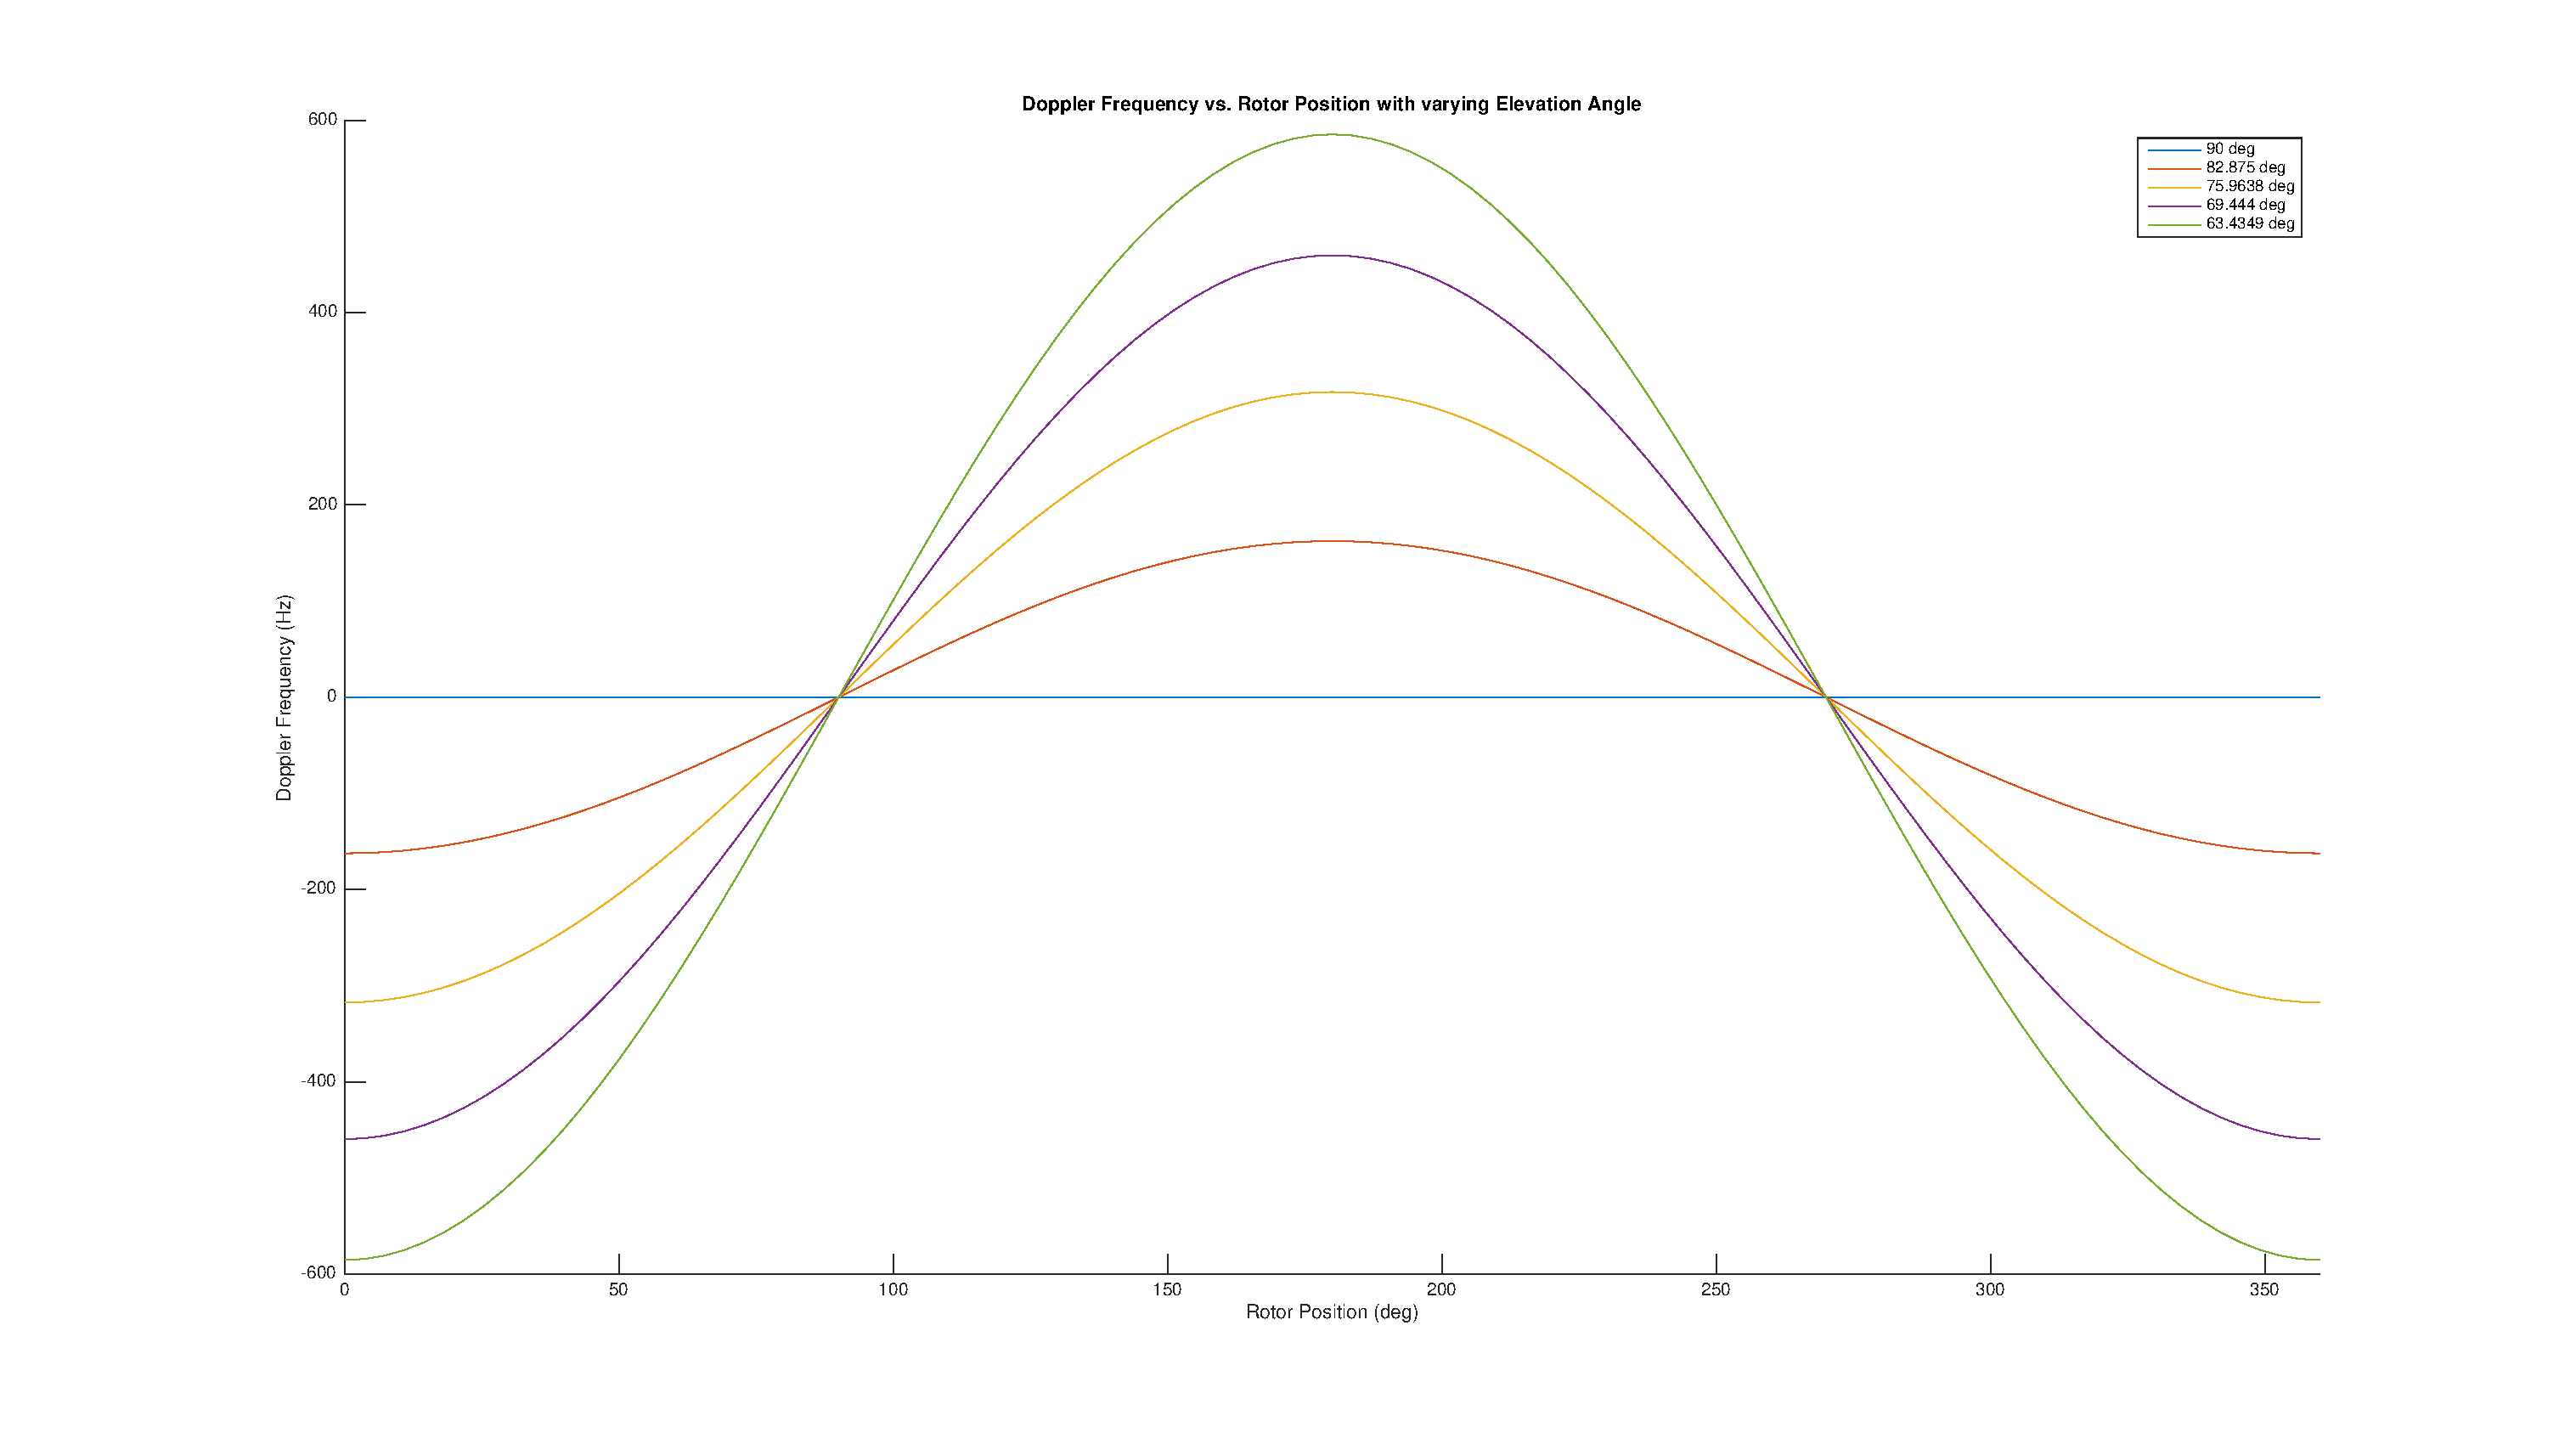
\includegraphics[width=10cm]{images/background/2d_theoretical_doppler_profile.eps}
		\caption{Doppler Frequency vs. Rotor Position with varying Elevation Angle}
		\label{fig:2D_theoretical_doppler}
	\end{center}
\end{figure}

Figure \ref{fig:2D_theoretical_doppler} shows the varying doppler frequency caused by the RBM at various elevation angles of the transmitter. The results of this is a sinusoidal doppler profile in which its amplitude increases as the elevation angle decreases. 

%validation consideration
Since this model has the receiver located at the axis of rotation this model can be seen as a special case of the next 3D models, this is because it is symmetric around the axis of rotation. Therefore any placement of the transmitter in 3D space can be distilled down to a 2D profile as such. This symmetry should then be mirrored in the ray tracing simulation as verification.

\subsection{3D Geometric Model}
The three dimensional geometric model is categorized by the position of the rotor blade and the position of the signal source. Since the rotor blade has a specific airfoil shape the models will take that into account through an approximation of that surface. The first model will be representative of having the transmitter inline with both the receiver and the blade, with the transmitter in both fore and aft positions. The next model will have the rotor approaching both the receiver and transmitter, and lastly the rotor will be receding from both the receiver and transmitter. All of the 3D models will have the receiver positioned offset from the axis of rotation.

\subsubsection{Transmitter inline with Receiver and Rotor Blade}
%go over the 3d model for the tx inline with blade fore and aft
The first two models as mentioned above fall under the criteria of the transmitter being inline with both the rotor blade and the offset receiver. 

Figure \ref{fig:3D_model_90az} depicts the transmitter at a 90\textdegree \space azimuth angle, which places it inline with the position of the receiver and the current location of the rotating blades. 

%describe the situation and the position of the objects
The objects in \ref{fig:3D_model_90az}  are similar to the ones previously stated in the 2D case. The X and Y axis are specifically drawn in blue and red respectfully, with the Z axis now the green dashed line and altitude is now denoted with a measurement bar. The receiver offset in the +Y direction is now stated. and the Blades are now colored gray. All other variables and colors denote their objects as previously stated in the 2D case. 

%3d pictures
\begin{figure}
	\begin{center}
		\includegraphics[width=15cm]{images/background/3d_geometry_tx_90az.eps}
		\caption{3D Geometric model with Tx at Azimuth angle of 90\textdegree}
		\label{fig:3D_model_90az}
	\end{center}
\end{figure}

%formulate the geometric equations
(equations doppler profile 90 deg)

%doppler profile result
\begin{figure}
	\begin{center}
		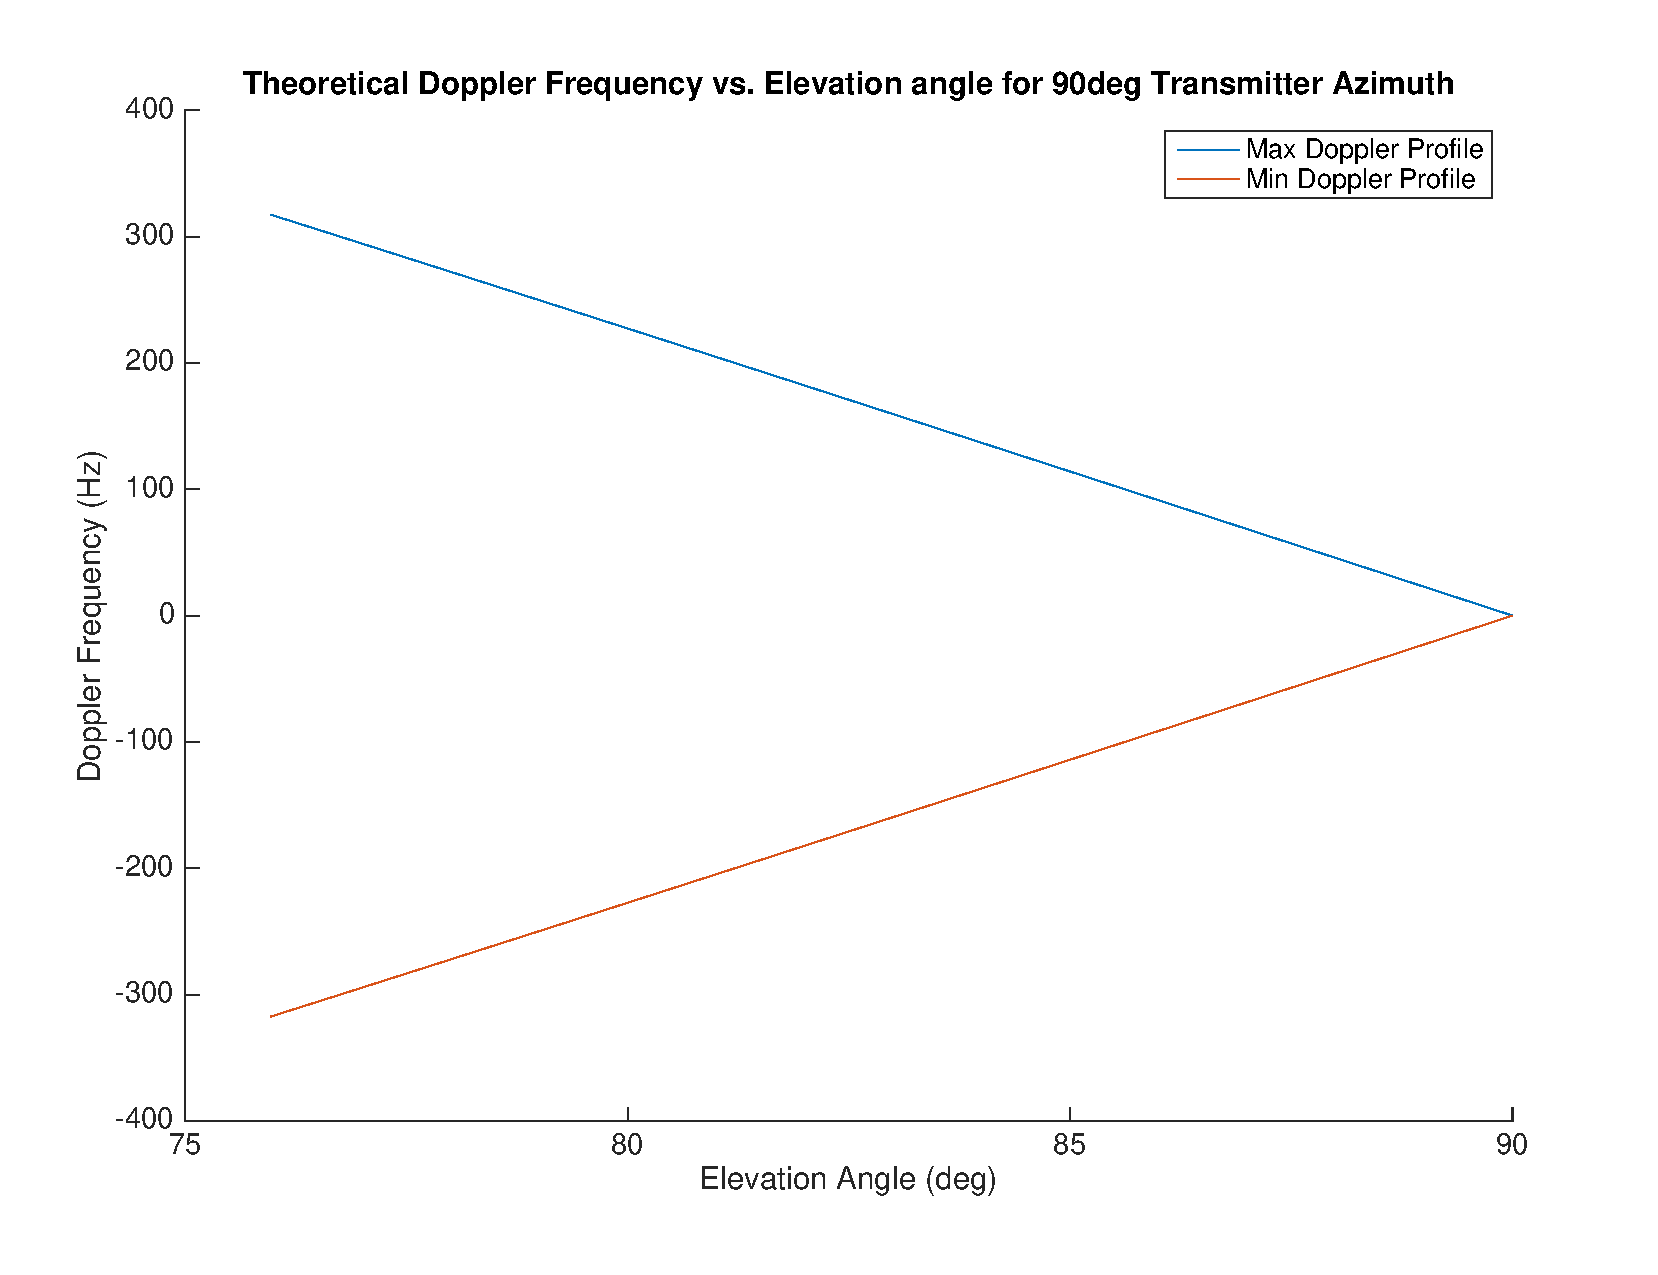
\includegraphics[width=10cm]{images/background/3d_geometry_tx_90az_doppler_profile.eps}
		\caption{Doppler profile of Tx at Azimuth angle of 90\textdegree}
		\label{fig:3D_model_90az_doppler}
	\end{center}
\end{figure}

Figure \ref{fig:3D_model_90az_doppler} shows the maximum and minimum doppler values versus elevation angle for a transmitter at an azimuth angle of 90\textdegree. The elevation angle is limited by the reflection angle, caused by the limited distance between the tip of the blade and the location of the receiver. This limitation constrains the doppler profile causing inaccurate transmitter elevation estimation at this transmitter azimuth position.

Figure \ref{fig:3D_model_270az} depicts the transmitter at a 270\textdegree \space azimuth angle, which places it inline with the position of the receiver and the current location of the rotating blades. This placement of the transmitter behind the helicopter is different from the situation in figure \ref{fig:3D_model_90az} because the value of $\theta_r$ is now not limited by the tip of the rotor and can go to smaller elevation angles.

\begin{figure}
	\begin{center}
		\includegraphics[width=15cm]{images/background/3d_geometry_tx_270az.eps}
		\caption{3D Geometric model with Tx at Azimuth angle of 270\textdegree}
		\label{fig:3D_model_270az}
	\end{center}
\end{figure}

%formulate the geometric equations
(equations doppler profile 270 deg)

%doppler profile result
\begin{figure}
	\begin{center}
		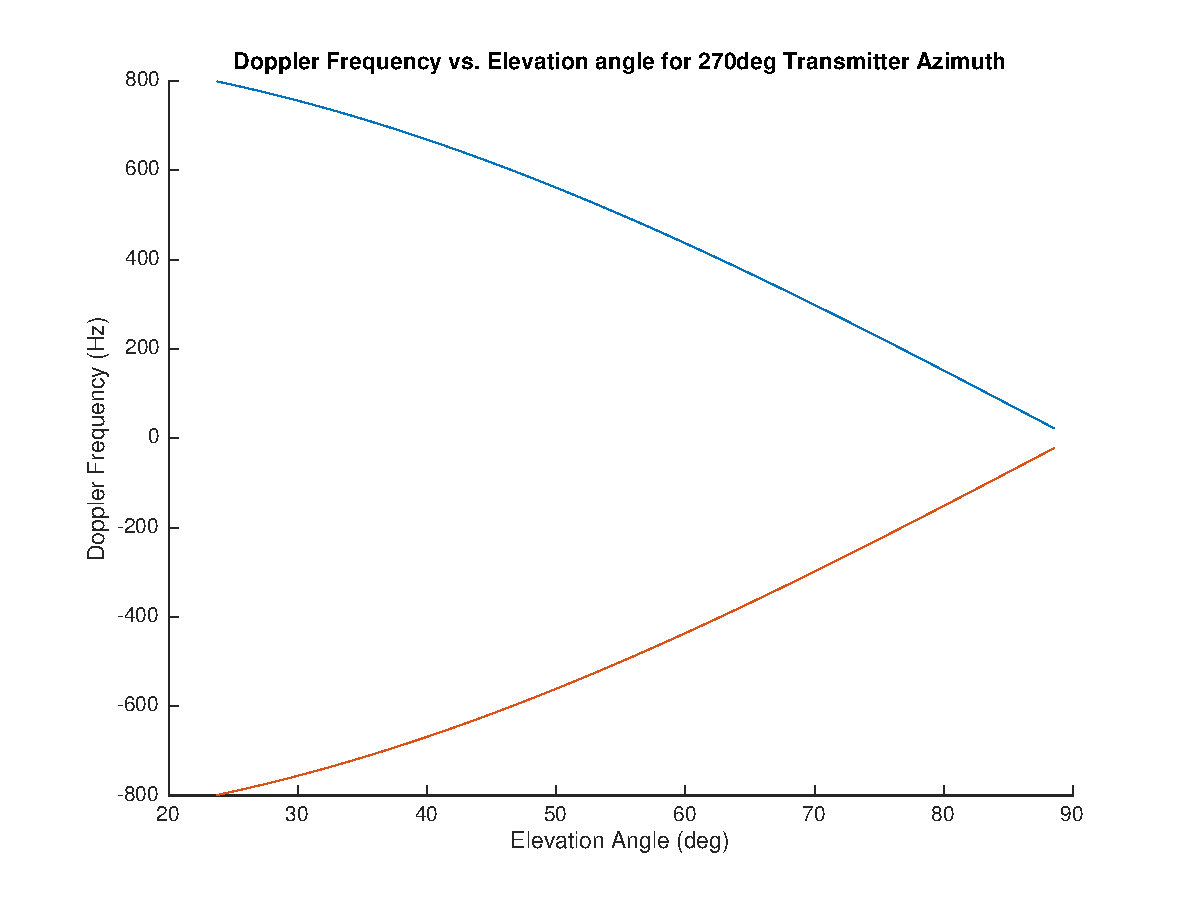
\includegraphics[width=10cm]{images/background/3d_geometry_tx_270az_doppler_profile.eps}
		\caption{Doppler profile of Tx at Azimuth angle of 270\textdegree}
		\label{fig:3D_model_270az_doppler}
	\end{center}
\end{figure}

Figure \ref{fig:3D_model_270az_doppler} shows the maximum and minimum doppler values versus elevation angle for a transmitter at an azimuth angle of 270\textdegree. The data from the figure is similar to the data from the previous figure \ref{fig:3D_model_90az} but does not exhibit the limitation on the reflection angle, allowing for smaller elevation angles and larger doppler shifts to occur.

\subsubsection{Approaching Model}
%go over the 3d model for the approaching blade
The approaching model shown in figure \ref{fig:3D_model_180az} depicts the transmitter at an azimuth of 180 \textdegree \space and the axis of X has now been rotated to be -X. The direction of the rotor blades is depicted ,in green, to follow the previous assumptions.

%describe the situation and the position of the objects
This case of the 3D model places the transmitter at 180 \textdegree \space so that the oncoming blades move toward both the receiver and the transmitter at the same time. This particular placement will cause a positive doppler profile because the blades will be moving in the direction of both objects, compressing the reflected wave accordingly.

%3d picture
\begin{figure}
	\begin{center}
		\includegraphics[width=15cm]{images/background/3d_geometry_tx_180az.eps}
		\caption{3D Geometric model with Tx at Azimuth angle of 180\textdegree}
		\label{fig:3D_model_180az}
	\end{center}
\end{figure}

%formulate the geometric equations
(equations doppler profile 180 deg)

%doppler profile result
\begin{figure}
	\begin{center}
		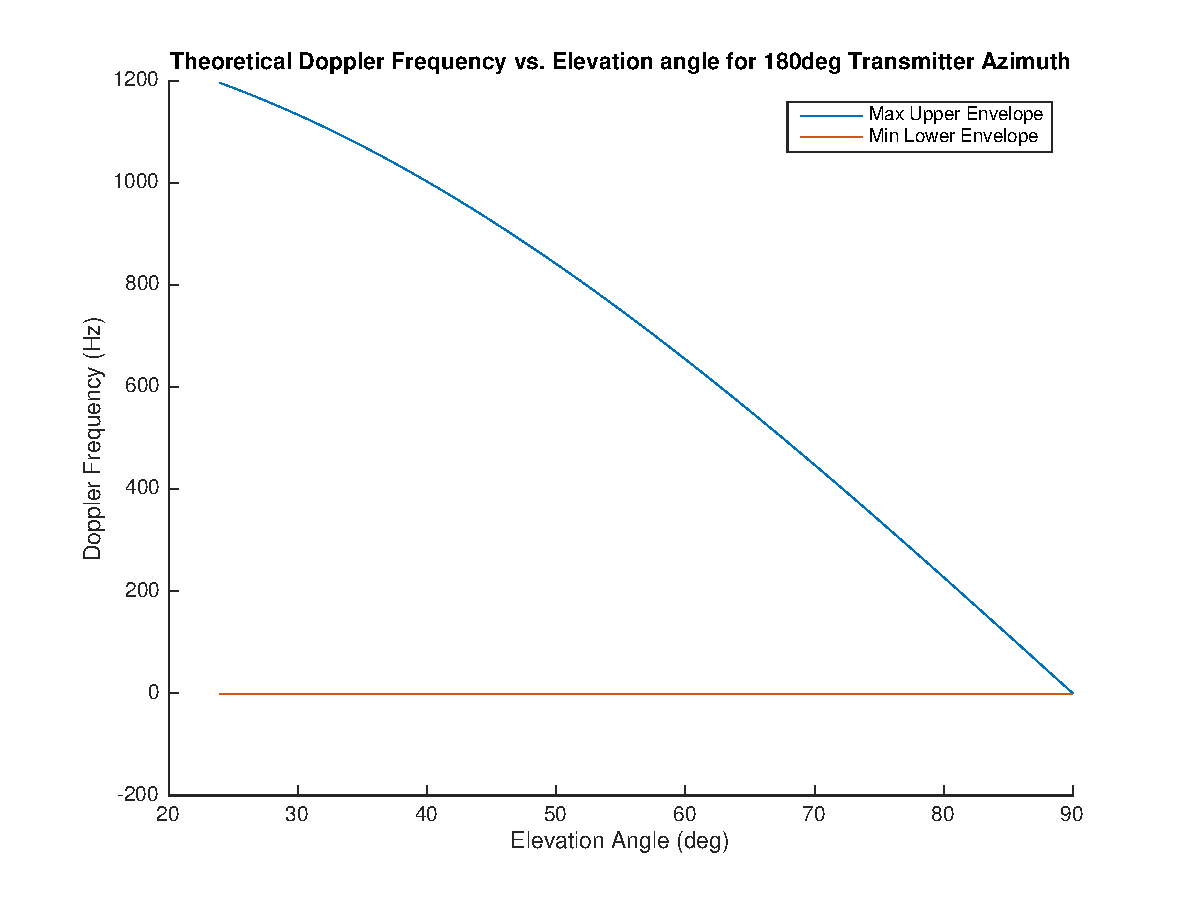
\includegraphics[width=10cm]{images/background/3d_geometry_tx_180az_doppler_profile.eps}
		\caption{Doppler profile of Tx at Azimuth angle of 180\textdegree}
		\label{fig:3D_model_180az_doppler}
	\end{center}
\end{figure}

Figure \ref{fig:3D_model_180az_doppler} shows the maximum and minimum doppler values versus elevation angle for a transmitter at an azimuth angle of 180\textdegree. The data from the figure shows the maximum of the doppler profile decrease as the elevation angle gets larger.

\subsubsection{Receding Model}
%go over the 3d model for the receding blade
The receding model shown in figure \ref{fig:3D_model_0az} depicts the transmitter at an azimuth of 0 \textdegree \space where the axis positions back to their original places and the direction of the rotor blade is now depicted in red.

%describe the situation and the position of the objects
This case of the 3D model places the transmitter at 0 \textdegree \space so that the receding blades move away from both the receiver and the transmitter at the same time. This particular placement should provide a negative doppler profile because the blades will be moving in the opposite direction of both objects, stretching the reflected wave accordingly.

%3d picture 
\begin{figure}
	\begin{center}
		\includegraphics[width=15cm]{images/background/3d_geometry_tx_0az.eps}
		\caption{3D Geometric model with Tx at Azimuth angle of 0\textdegree}
		\label{fig:3D_model_0az}
	\end{center}
\end{figure}

%formulate the geometric equations
(equations doppler profile 0 deg)

%doppler profile result
\begin{figure}
	\begin{center}
		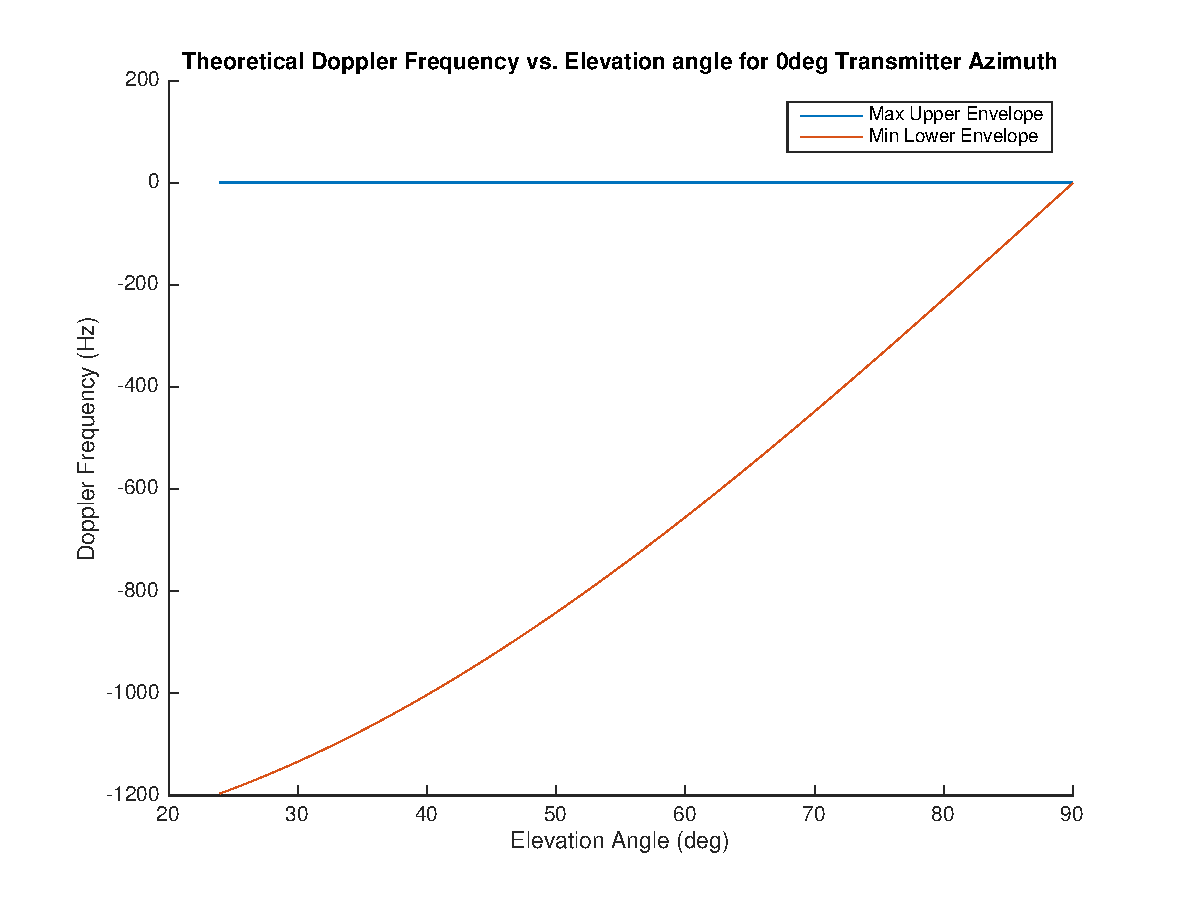
\includegraphics[width=10cm]{images/background/3d_geometry_tx_0az_doppler_profile.eps}
		\caption{Doppler profile of Tx at Azimuth angle of 0\textdegree}
		\label{fig:3D_model_0az_doppler}
	\end{center}
\end{figure}

Figure \ref{fig:3D_model_0az_doppler} shows the maximum and minimum doppler values versus elevation angle for a transmitter at an azimuth angle of 0\textdegree. The data from the figure shows the minimum of the doppler profile increase as the elevation angle gets larger.




\clearpage  %Start a new page
\lhead{\emph{Radio Propagation Simulation}}
\chapter{Radio Propagation Simulation} \label{ch:radio_propagation}

\section{Introduction}
%introduce the section and what will be discussed here
The simulation software is broken down into three main components, the radio wave propagation model, the scene model, and the ray tracing engine. The wave propagation model is a collection of equations that describe the physical phenomena that affect the propagation when represented by rays. The model used is based upon classical geometric optics to work with the ray tracing engine. The scene model is comprised of a 3D environment in order to define the physical rotor blade surface. The receiver and transmitter will also be defined in the same environment with simulated characteristics to match real life conditions. The ray tracing engine uses recursive execution described in \cite{Whitted1979}, replacing cameras and lights for receivers and transmitters respectively in a three dimensional environment.

\section{Radio Propagation Model}
%define the math behind the physical laws that are simulated within the simulation
The propagation model defined in this project is based on the following physical phenomena; free-space path loss, reflection, and the doppler effect. They are all formally established models described in full in \cite{Bertoni1999}, \cite{Parsons2000}, and \cite{Willis2005}. Although several effects are described within the model several were left out to simplify the computation due to the overhead of implementation in 3D space and because of the assumptions made about the scene model.

\subsection{Free-Space Path Loss}
%describe path loss
Free-Space path loss is calculated using the Friis transmission and is incorporated into the model by keeping track of the distance a ray travels and adjusting its power is

%FSPL formula
\begin{equation}
	 P_r = G_r G_t P_t \left (\frac{\lambda}{4\pi R}\right)^2
	 \label{eqn:FSPL}
\end{equation}

%formula description
where $P_r $ is the power at the receiver, $P_t$ is the power at the transmitter, $G_r$ and $G_t$ are the antenna gains, 
$\lambda$ is the wavelength, and $R$ is the distance between the receiver and transmitter antennas. In the simulations described in this paper, $G_r$ and $G_t$ are assumed to have a value of 1.

\subsection{Reflection}

\subsubsection{Specular Reflection}
In the case of a perfect reflection the angle of the reflection is calculated by

%Spec formula
\begin{equation}
	\theta_r = \cos^{-1}(\vec{n} \bullet (-\vec{d_i}))
	\label{eqn:spec}
\end{equation}

%formula description
where $\theta_r$ is the angle of the reflected ray, $\vec{n}$ is the normal vector to the surface, and $\vec{d_i}$ is the direction vector of the incident ray.

\subsubsection{Reflection Loss}
Power loss due to surface reflection is described through the following coefficient

%Reflection loss formula
\begin{equation}
	\Gamma = \frac{\cos(\theta_i) - \sqrt{\varepsilon}\cos(\theta_t)}{\cos(\theta_i) + \sqrt{\varepsilon}\cos(\theta_t)}
	\label{eqn:RL}
\end{equation}

%formula description
where $\theta_i$ is the angle of incidence with the object's surface normal, $\varepsilon$ is the dielectric constant for that surface, and $\theta_t$ is the angle of refraction as described by Snell's law

\begin{equation}
	\theta_t = \sin^{-1}\left(\frac{\sin(\theta_i)}{\sqrt{\varepsilon}} \right)
	\label{eqn:snell}
\end{equation}

The final reflected power is then

\begin{equation}
	P_{reflected} = P_i|\Gamma|
	\label{eqn:reflected_power}
\end{equation}

%reflection power loss description
where $P_i$ is the incident power before reflection loss.

\subsubsection{Diffuse Reflection}
A perfect diffuse reflection, also known as Lambertian reflection, will reflect rays in all directions in a uniform hemisphere \cite{Sizun2005}. The hemisphere is centered at the point the ray hits, producing rays away from the surface. To approximate a particular type of surface the rays power is attenuated by the surface's bi-directional reflectance distribution function (BRDF) \cite{Suffern2007}, \cite{Pharr2010}, \cite{Glassner1995}. There are several ways of calculating the BRDF, but the simplest is the Phong BRDF which will be used in this ray tracing implementation \cite{Phong:1998:ICG:280811.280980}. This method for the BRDF is regularly used in the rendering of computer graphics to simulate the reflection of light off surfaces and combines the diffuse and specular components. Since this was not designed for the longer wavelengths used in RF communications, an assumption is made about surface features. Where features relevant to light waves,  produce a reflectance distribution similar for this application. 

%The BRDF parameters were then selected to be frequency independent to form a plausible reflectance distribution for the physical effects.

%multipath fading
\subsection{Fading}
The transmitted signal power experiences fading described by

\begin{equation}
	F = cos\left(2\pi \frac{d}{c} + t_0\right)
	\label{eqn:fading_coeff}
\end{equation}

where $F$ is the fading coefficient, $d$ is the total distance the particular ray has traveled, $c$ is the speed of light, and $t_0$ is the starting time of the current frame. The power can then be calculated using

\begin{equation}
	P_{faded} = PF
	\label{eqn:power_faded}
\end{equation}

where $P_{faded}$ is the adjusted power due to fading and $P$ is the signal power. The superposition of each ray's faded power becomes the received signal.

\subsection{Doppler Effect}
%define doppler effect
The Doppler effect is characterized by

%Doppler formula
\begin{equation}
	f = \left ( \frac{c + v_r}{c + v_s} \right ) f_0
	\label{eqn:formalDop}
\end{equation}

It is assumed that both the receiver and the transmitter are not moving therefore, the only Doppler imparted on the signal will be from the rotation of the blades. The associated Doppler is calculated using

%formula for doppler on the rotor blade.
\begin{equation}
	f = f_0 + \frac{v_t + v_r}{\lambda} %reradiated after reflection
	\label{eqn:observedShift}	
\end{equation}

where $f_0$ is the initial transmitted frequency, $\lambda$ is the wavelength, $v_t$ is the velocity in the direction of the transmitter, and $v_r$ is the velocity in the direction of the reflection. This is similar to the Bistatic radar equation for Doppler, but since the reflection is not guaranteed to be toward the receiver we calculate the doppler as it makes contact with the surface and as it is re-radiated according the blades direction of travel.

\begin{equation}
	\lambda = \frac{c}{f_0}
	\label{eqn:wavelength}
\end{equation}

where $\lambda$ is the wavelength of the transmitted signal based off of the speed of light $c$ and its initial frequency $f_0$

\begin{equation}
	v_t = r \omega_r (\vec{d_p} \bullet \vec{d_t})
	\label{eqn:v_t}
\end{equation}

%formula description
where $r$ is the radius along the length of the blade where the reflection occurs. $\omega_r$ is the angular velocity of the rotor. $\vec{d_p}$ is the normalized vector that is perpendicular to the rotor in its direction of travel and $\vec{d_t}$ is the normalized vector that is in the direction of the transmitted ray.

\begin{equation}
	v_r = r \omega_r (\vec{d_p} \bullet \vec{d_r})
	\label{eqn:v_r}
\end{equation}

where $\vec{d_r}$ is the normalized vector that is in the direction of the reflected ray.

\section{Scene Model}
% describe what the scene model is and how it will fit in to the ray tracer and the 3d setting
The scene model is the 3D environment in which the physical objects are placed. 
The model is comprised of three types of objects; the rotor blades, transmitter and receiver. The rotor blade is the most complex object due to its airfoil shape. The transmitter is a point source that projects the rays into the scene, and the receiver is described in a similar fashion with a surrounding boundary layer. There are no other objects within the scene. This is because the effect of the rotor on the received signal is analyzed for defining characteristics without outside variables.

\subsection{Rotor Blade}
%go over the shape of the blade
The rotor blade is the most complex object within the scene, due to its airfoil shape. The airfoil shape is designed to produce lift for the helicopter, and designing one is outside the scope of this project. Fortunately, there are databases that provide real helicopter airfoil designs in x,y coordinates. This data forms a 2D cross-section of the airfoil shape that will be extruded into the length of the rotor blade. Figure \ref{fig:airfoil} shows the airfoil cross-section that will be used to create the rotor surface. 

%figure of 2D airfoil
\begin{figure}
	\begin{center}
		\includegraphics[width=15cm]{images/radio_propagation/2d_airfoil.png}
		\caption{Airfoil Cross-Section}
		\label{fig:airfoil}
	\end{center}
\end{figure}

%go over how it is formed and the tessellation code
The 2D airfoil sections will form the ribs of the rotor blade but the surface of the blade will be made up of primitive surfaces to approximate the curved airfoil shape. The primitive shapes are triangles that span between the ribs and go around to cover the surface. This was done using a lightweight mesh generation method using a priori knowledge of the blade's shape. The designed algorithm, located in \ref{class_blade__surface_a160959f632ad73eff846aeea81aa84ae} $create\_surface()$ method, takes advantage of the object's uniform structure in 2D. The surface normals are then adjusted to match the correct directionality. Figure \ref{fig:tessilation} shows the created surface for the rotor blade that will be used in the scene.

%figure of tessilation
\begin{figure}
	\begin{center}
		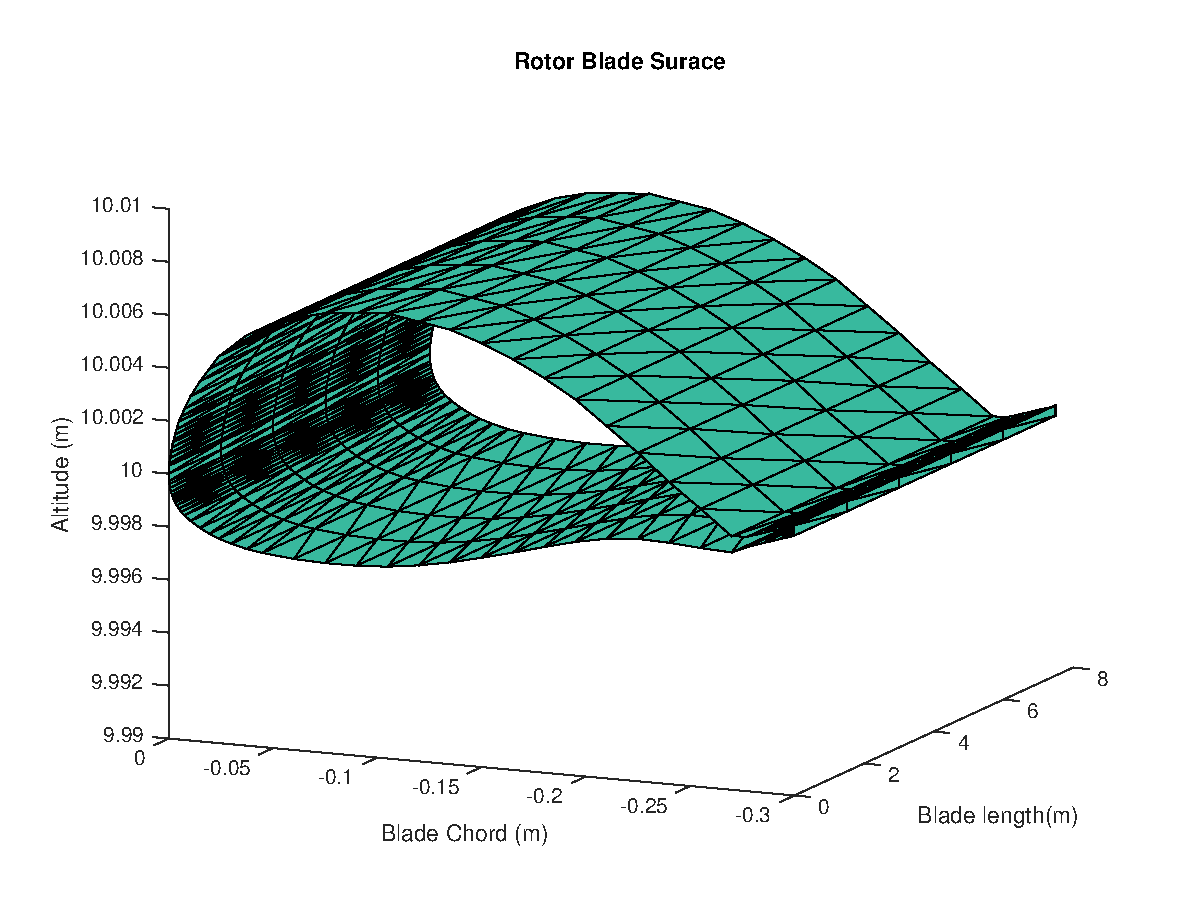
\includegraphics[width=15cm]{images/radio_propagation/blade_surface_tesselation.eps}
		\caption{Blade Surface Tessilation}
		\label{fig:tessilation}
	\end{center}
\end{figure}

%modular parameters
All aspects of the rotor blade are parameterized. Starting with the airfoil shape, which is defined by a set of 2D coordinates. The length and the number of rib sections can be configured along with the number of blades and corresponding altitude. As well as the RPM. This allows the scene to replicate any type of rotor configuration and position it at a specific altitude.

\subsection{Transmitter}
%point source transmitter casting rays in specific direction
The transmitter is modeled as a point source, this means that all the radio waves are projected from this point into the scene. It is assumed that the transmitter is located on the ground within the x,y plane in relationship to the rotor blades. The transmitter is configured with a center frequency and is assumed to produce a tone at that frequency. Therefor, the signal produced has no inherent modulation applied to it.
%direction creation
Being that the transmitter is emitting radio waves into a 3D space, it is assumed to be transmitting in an omnidirectional fashion. But because the rotor and the receiver are the only two other objects within the scene, radio waves will only be propagated in their direction. This limitation allows for a higher concentration of rays to be casted, resulting in a higher resolution picture that eliminates computational overhead for the tracing engine. Figure \ref{fig:transmitter_direction} shows the rays, in blue, casted only in the vicinity of the rotor blade and receiver.

%figure of transmitter direction
\begin{figure}
	\begin{center}
		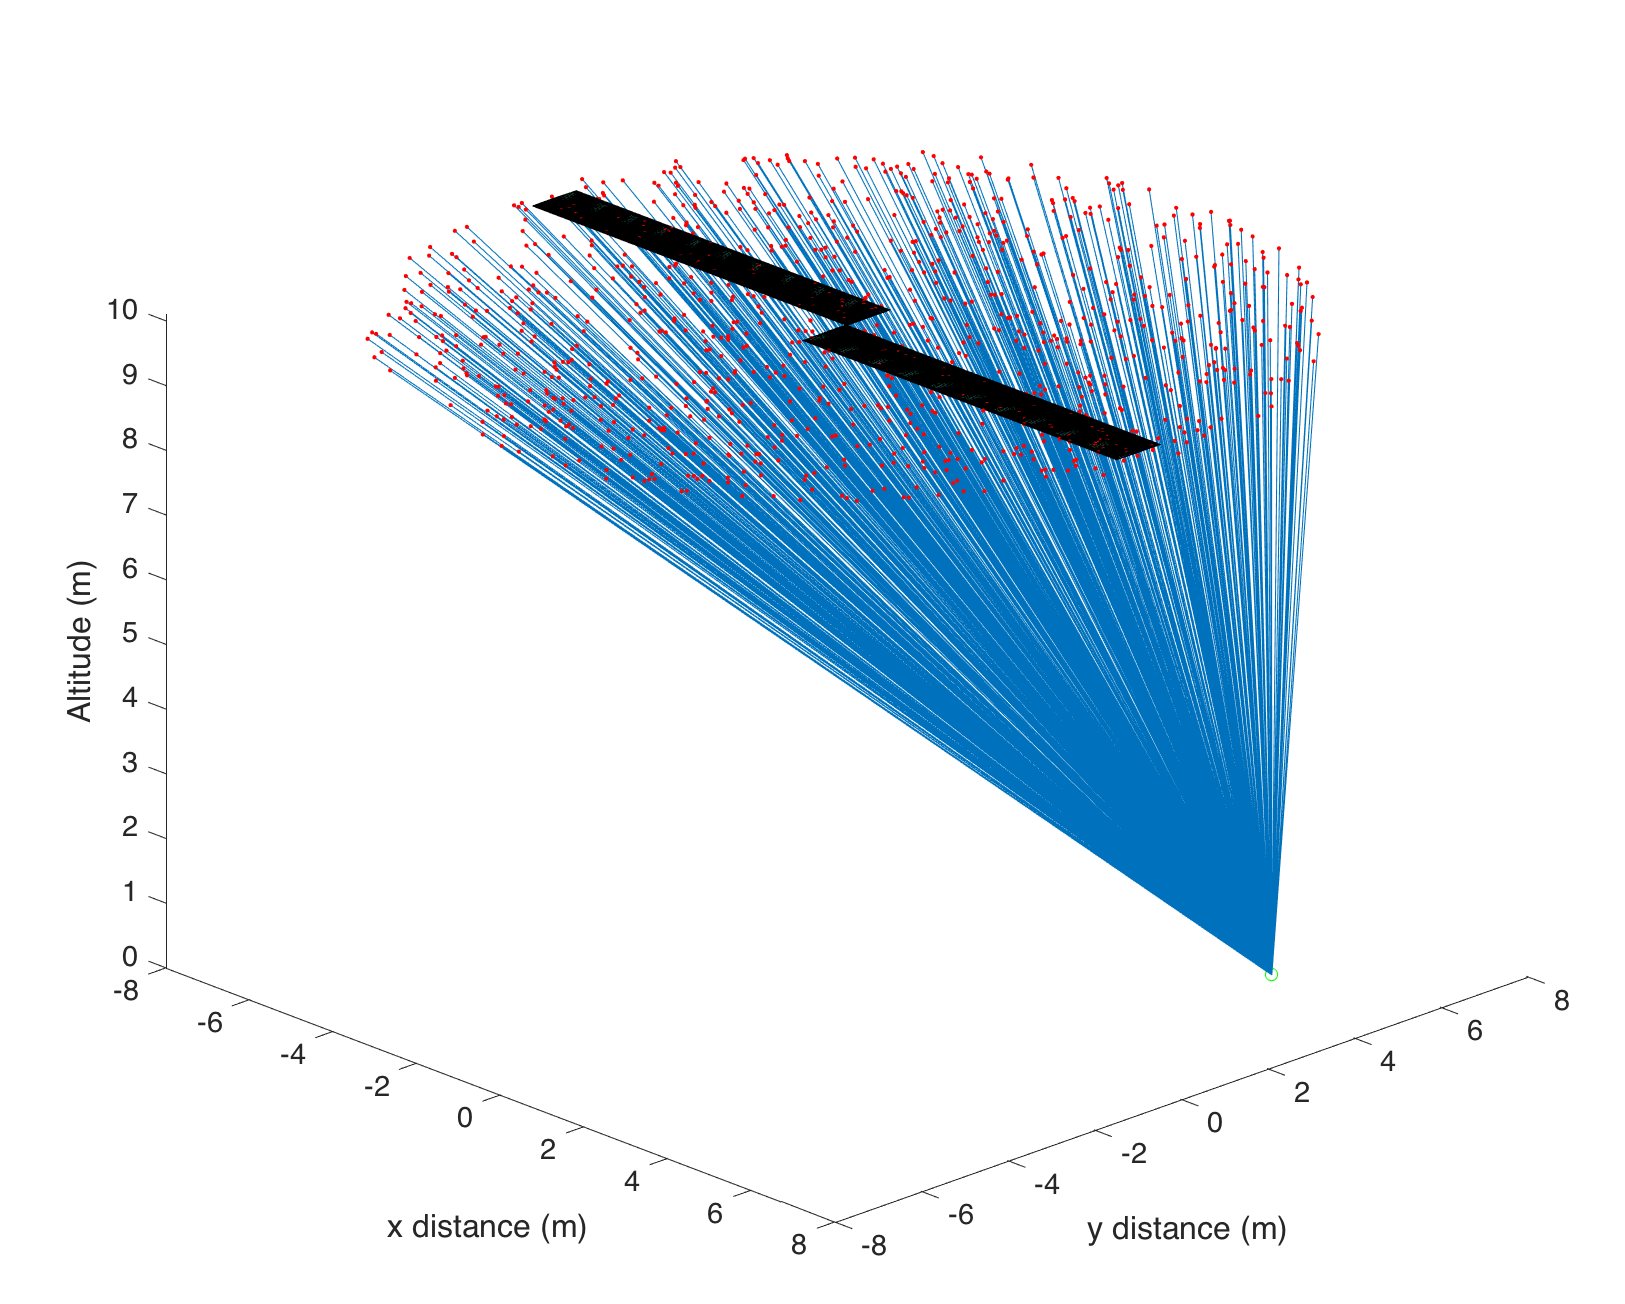
\includegraphics[width=15cm]{images/radio_propagation/transmitted.eps}
		\caption{Transmitter Rays}
		\label{fig:transmitter_direction}
	\end{center}
\end{figure}

\subsection{Receiver}
%physical receiver dimensions and antenna chars
The receiver object is modeled as a point in 3D space with a surrounding boundary layer in the shape of a sphere. This is because the receiver is assumed to have an omnidirectional antenna which will receive radio waves from all directions uniformly. The receiver will record any ray that hits the boundary layer within each frame of the simulation to create a sample of data at that instance in time.
%processing in each frame
The sample is produced using superposition of all the rays that are acting on the receiver at that instance in time which are then extrapolated to produce a clear result.
%realism
The receiver is configurable allowing the user to set a desired center frequency along with the sampling rate of the simulated hardware. The sampling rate will determine several simulation parameters in the ray tracer due to the need to associate this rate with the change in the rotor position for the next frame. The consequence of this is that increasing the sample rate will produce higher resolution results but will increase the computational overhead of the simulation.

\section{Ray Tracing}
%describe the core tracing engine and describe the flow of the program
The ray tracing simulation is conducted in the Monte Carlo fashion acting on the scene and propagation models. This method of raytracing is established for creating realistic images in \cite{Suffern2007}, \cite{Pharr2010}. The simulation is performed over successive iterations. Each iteration is a discrete element called a frame and each frame will be updated to represent the change in the position of the rotor blade.

\subsection{Computation}
%flow of the program
The ray tracing engine first sets up the environment, creating the surfaces and placing the objects in the scene. Then the number of frames that will be computed. The number of frames is determined by the number of rotations that the rotor makes within the simulation, the speed of the rotor in RPM and the sampling frequency of the receiver defined before the beginning of the simulation. This is described by

%frame rates equation
\begin{equation}
	Frames = \frac{60  f_s}{RPM} Rev
	\label{eqn:frames}
\end{equation}

where $Frames$ is the number of frames that will be computed in the simulation, $f_s$ is the sampling frequency of the receiver, $RPM$ is the revolutions per minuet of the rotor, and $Rev$ is the number of revolutions that the rotor makes in the simulation.

In each frame a set number of rays are casted into the scene in a uniformly distributed circle in the direction of the rotor and receiver using

%uniform disk equation
\begin{equation}
	v_{ray} = \begin{bmatrix}
			x \\
			y \\
			z \\
	\end{bmatrix}
	= \begin{pmatrix}
			\sqrt{r} \cos{\theta_u}  + d_x\\
			\sqrt{r} \sin{\theta_u}  + d_y \\
			d_z \\
	\end{pmatrix}
	\label{eqn:disk}
\end{equation}

The casting technique reduces the computation overhead by limiting the search space. It also creates a higher resolution result by focusing the limited number of rays in the direction of the other objects shown in figure \ref{fig:samp_method}.

%figure of casting disk
\begin{figure}
	\begin{center}
		\includegraphics[width=15cm]{images/radio_propagation/sampling_method.eps}
		\caption{Disk Sampling Method}
		\label{fig:samp_method}
	\end{center}
\end{figure}

When a ray is casted into the scene it has an origin point, a direction vector, a frequency, and an initial power level. The ray then travels through the scene till it encounters another object. If there is a collision with the receiver it is recorded. If the ray collides with a rotor blade a new ray is calculated based on the normal of the geometric surface. The new ray's power is then updated as well as an updated frequency since the blade is moving. The power level is adjusted based on the BRDF of the specific material. Due to only the rotor and receiver being in the scene, rays that are found to hit the rotor are reflected, then a dedicated ray in the direction of the receiver is also calculated with a decayed power and adjusted frequency respective to the reflection.

\subsection{Output}
%iq samples
The superposition of these receiver contributions during each frame creates the received signal data. The received signal data will then be visualized in spectrograms over the length of the simulated time. The simulation does not render in real time but instead creates a Comma Separated Value (CSV) file of In-phase and Quadrature (IQ) data that can then be loaded into MATLAB for signal processing.






\clearpage
\lhead{\emph{Received Signal Simulation}}
\chapter{Received Signal Simulations} \label{ch:simulations}
%define the signal characteristics and evaluate the properties of the resulting signal over the parameter sweeps

\section{Introduction}
The following simulations performed will define the search space on the effect of rotor blade modulation. Since the software developed allows for full parameterization of the objects within the scene the simulations will focus on a few that effect the different object's positions in 3D space and the resulting received signal. The parameters that will be changed are the position of the receiver, pitch of the rotor blade, and transmitter position. The effect of each parameter will be analyzed to determine what information can be derived for localization.

%-----------------------------------------------------------------------------------------------------------------------------------------------------------------------

\section{Analysis Techniques}
The data from the .CSV files generated by the raytracing program is loaded into MATLAB scripts to process the data. The technique that is used is the spectrogram function that computes the short time Fourier transform. This allows for computations to be done in the time frequency domain and provide an accurate picture of how the signal is changing with time. The following figure \label{fig:test_spec} shows an example of the computed spectrograms.

%short Fourier transform alg

\begin{figure}
	\begin{center}
		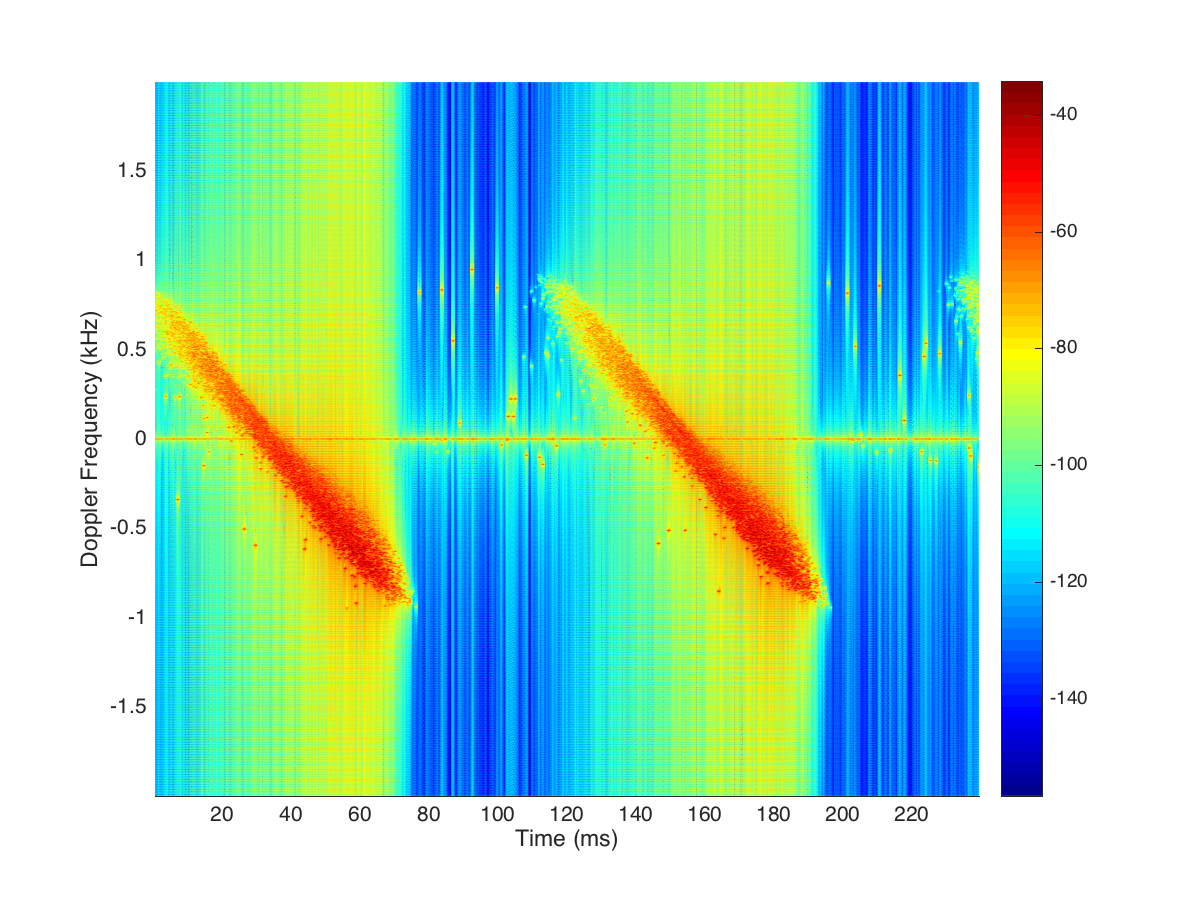
\includegraphics[width=10cm]{images/simulation/test_analysis_spectrogram.eps}
		\caption{Example Spectrum for one Blade revolution with transmitter at Azimuth of 45\textdegree \space and Elevation of 35\textdegree}
		\label{fig:test_spec}
	\end{center}
\end{figure}

After the computation of the short time Fourier transform the doppler envelope is calculated by performing a threshold on the power, in both the positive and negative doppler, at each time slice. The envelope value for that time slice is found by approaching zero frequency and stopping as the power reaches a predetermined level from both the negative and positive values. The power level to set the threshold is calculated differently based on weather the elevation or the azimuth parameter is being swept. For the azimuth angle sweep, which will be shown later in section \ref{taa}, the maximum power is found in each time slice then those values are averaged. Then for each successive angle the same average is taken and averaged with all the others 

%equation for power averaging over successive angles

This technique is used because the elevation angle is remaining constant, so the distance with the helicopter platform should be constant as well. When varying the elevation angle in section \ref{sec:tea} the same method cannot be used because the distance is changing so only the maximum power is found in each time slice then those values are averaged without any successive averaging.

\begin{figure}
	\begin{center}
		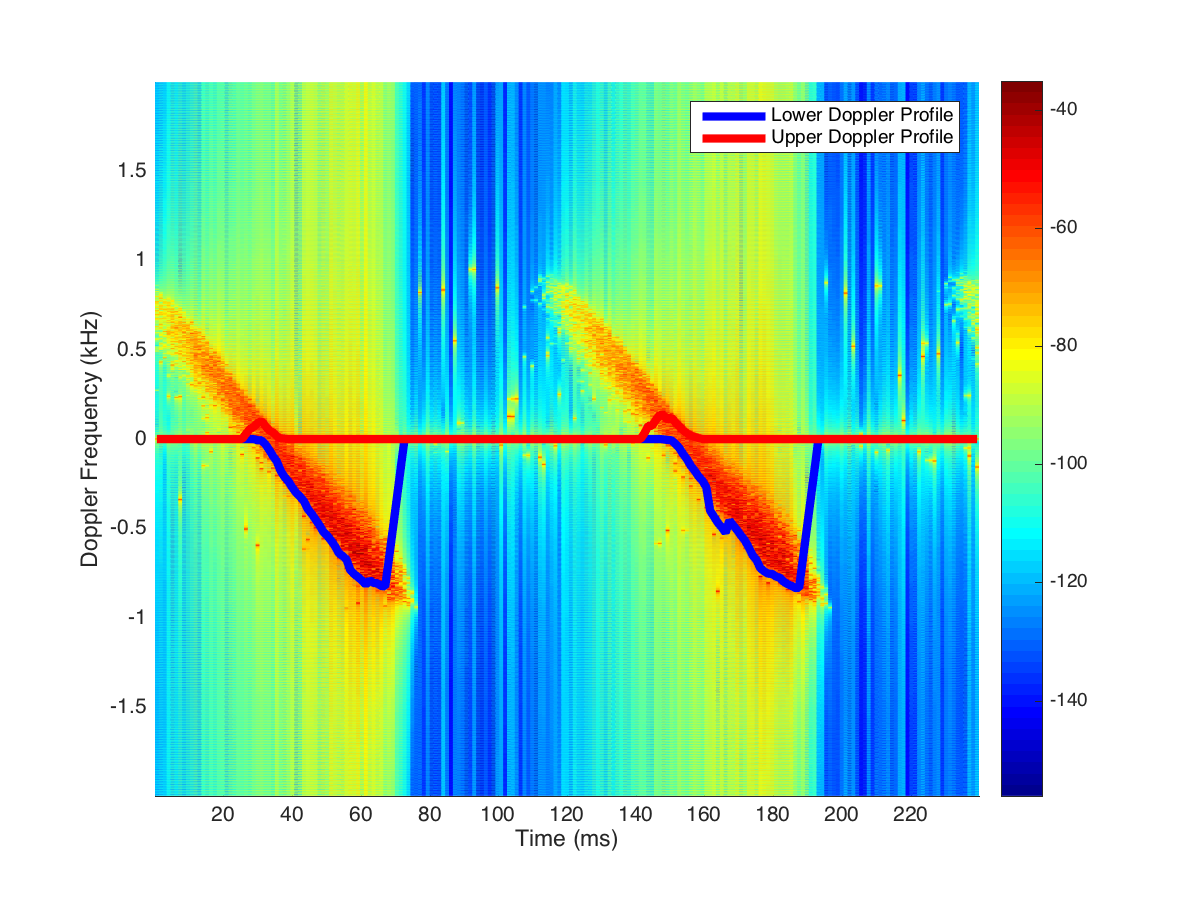
\includegraphics[width=10cm]{images/simulation/test_analysis_spectrogram_with_envelope.eps}
		\caption{Example Spectrum with Doppler Profile for one Blade revolution with transmitter at Azimuth of 45\textdegree \space and Elevation of 35\textdegree}
		\label{fig:test_spec_w_doppler_profile}
	\end{center}
\end{figure}

The Doppler envelopes are displayed in figure \ref{fig:test_spec_w_doppler_profile}, the lower in blue and the upper in red. The minimum is calculated from the lower envelope, and the maximum from the upper envelope. Those values are then used to characterize that doppler profile and analyze signal trends as different variables change.

%-----------------------------------------------------------------------------------------------------------------------------------------------------------------------
\section{Receiver Position}
%display spectrograms of the rx position and its affect on doppler and pick a value 7m for all subsequent tests
%use reasoning on cleaner signal more signal variation.
The position of the receiver is determined ultimately by its location on the physical aircraft. The position can be anywhere along the length of the body of the helicopter, but for the purpose of the simulation the receiver position will be varied from directly underneath the rotor to just past the tip. 

%figure of the receiver position 0 to 9m
\begin{figure}
	\begin{center}
		\includegraphics[width=9cm]{images/simulation/rotor_rx_position.eps}
		\caption{Position of the Receiver in Relation to the Rotor Blades}
		\label{fig:rx_position_image}
	\end{center}
\end{figure}

The rotor blade length from figure \ref{fig:rx_position_image} is 7.5m so the receiver will be varied from 0m to 9m in 1m increments. The resulting signal is analyzed by calculating its doppler envelope. Then the maximum and minimum of that envelope will then be used to determined the overall effect of the position of the receiver.

%figure of maximum doppler vs rx position
\begin{figure}
	\begin{center}
		\includegraphics[width=10cm]{images/simulation/receiver_position_max_doppler.eps}
		\caption{Max and Min Doppler vs. Receiver Position with Tx Azimuth at 135\textdegree \space and Elevation at 54\textdegree}
		\label{fig:rx_position}
	\end{center}
\end{figure}
%azimuth = 135, elevation = 54deg

The figure \ref{fig:rx_position} shows maximum doppler vs the position of the receiver. From this graph the maximum doppler frequency changes significantly as the receiver is moved from directly under neath the rotor to past the tip of the rotor at 9m.The position of the receiver also effects the resulting signal envelope shapes shown in figures \ref{fig:rx_position_0m} and \ref{fig:rx_position_7m}.

%figure of spectrogram at 0m -- figure of spectrogram at 7m side by side
\begin{figure}
	\begin{center}
		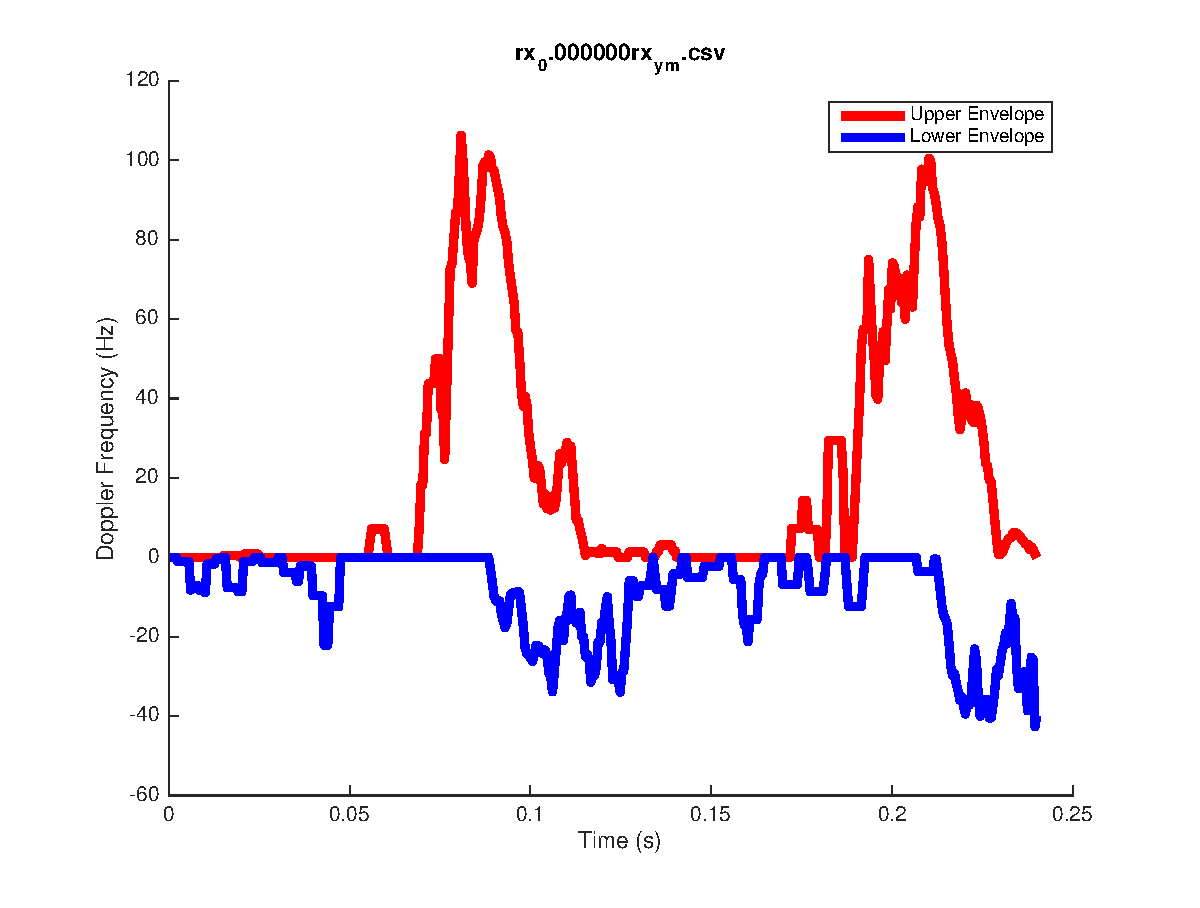
\includegraphics[width=10cm]{images/simulation/Doppler_Receiver_0m.eps}
		\caption{Doppler Envelope with receiver at 0m}
		\label{fig:rx_position_0m}
	\end{center}
\end{figure}

\begin{figure}
	\begin{center}
		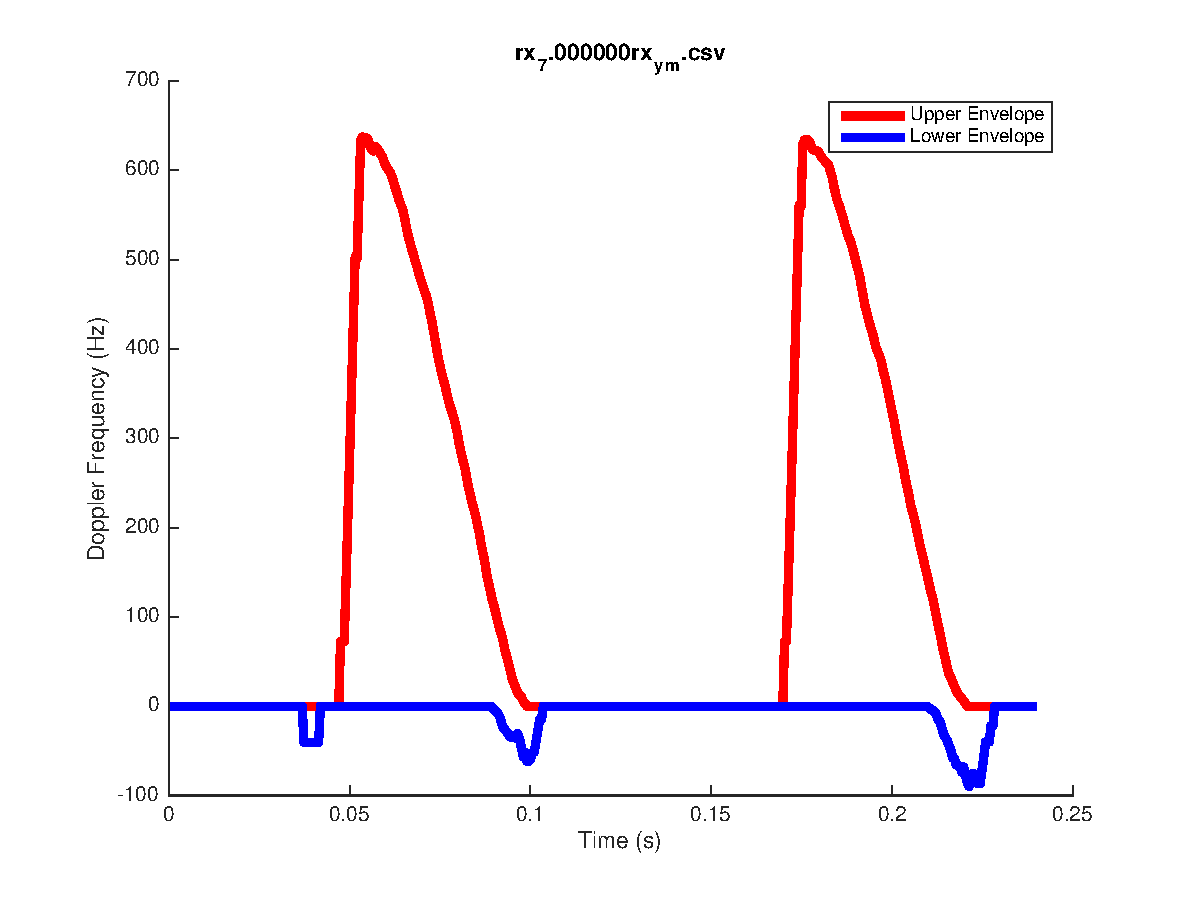
\includegraphics[width=10cm]{images/simulation/Doppler_Receiver_7m.eps}
		\caption{Doppler Envelope with receiver at 7m}
		\label{fig:rx_position_7m}
	\end{center}
\end{figure}

Comparing figure \ref{fig:rx_position_0m} with \ref{fig:rx_position_7m} the max doppler reflects the information in figure \ref{fig:rx_position} and the overall envelope is afected. The envelope in figure \ref{fig:rx_position_0m} is much noiser than the envelope of figure \ref{fig:rx_position_7m} and the envelope of this second figure has a more distinct shape with less variation between its two peaks. The position of the receiver will also determine whether the azimuth angle can be derived from the resulting signal shown later in section \ref{taa}. Therefore the receiver will be offset from the center of rotation by 7m for the subsequent simulations.


%-----------------------------------------------------------------------------------------------------------------------------------------------------------------------
\section{Rotor Pitch}
%display spectrograms of rotor pitch from 0 to -15 deg nominal value, then evaluate the effect.
%try to show that pitch does not change the signal significantly
The pitch of the rotor blades determines the amount of lift the rotors create. The pitch range is determined by the shape of the airfoil and the angle at which it will stall and no longer produce lift. For the purpose of the simulations, and the selected airfoil, the pitch range will be from 0\textdegree  \space to 15\textdegree.

%figure of pitched airfoil at 0 and at 15 deg
\begin{figure}
	\begin{center}
		\includegraphics[width=9cm]{images/simulation/pitch.eps}
		\caption{Rotor Pitch}
		\label{fig:blade_pitch}
	\end{center}
\end{figure}

The resulting signal is analyzed by calculating its doppler envelope. Then the maximum and minimum of that envelope will then be used to determined the overall effect of pitching the rotor blade. 

%figure of doppler vs pitch
\begin{figure}
	\begin{center}
		\includegraphics[width=10cm]{images/simulation/pitch_max_doppler.eps}
		\caption{Max and Min Envelope Frequencies vs Rotor Pitch with Tx Azimuth at 135\textdegree \space and Elevation at 54\textdegree}
		\label{fig:pitch_15_135deg}
	\end{center}
\end{figure}
%azimuth = 135deg, elevation = 54deg

From figure \ref{fig:pitch_15_135deg} the effect of pitch on the maximum doppler frequency is a linear increase between a pitch from 0 \textdegree \space to 15\textdegree. Due to the linear increase the pitch of the rotor blade can be accounted for when making measurements on subsequent simulation analysis. One issue does arise in when the transmitter is located underneath the helicopter which is shown in figure \ref{fig:pitch_tx0}.

%figure of tx_0 and increasing pitch slope?
\begin{figure}
	\begin{center}
		\includegraphics[width=10cm]{images/simulation/pitch_0txPos_max_doppler.eps}
		\caption{Max and Min Envelope Frequencies vs Rotor Pitch Transmitter Underneath the Helicopter}
		\label{fig:pitch_tx0}
	\end{center}
\end{figure}
%azimuth undefined, elevation 90deg

As the pitch increases linearly at first then climbs at a much faster rate. This offset when the transmitter is directly underneath is caused by the pitch of the blade reflecting rays into the receiver which would be reflected back at the ground if the pitch was 0\textdegree. If the assumption is that the helicopter is hovering when these measurements take place the pitch of the rotor will be much less than the maximum pitch available. This assumption will adjust the maximum pitch to 15 \textdegree \space which will allow for the linear assumption to be fulfilled even when the transmitter is directly underneath the helicopter.

%figure max doppler vs range of 15 and 7.5 pitch and 0 pitch side by side
\begin{figure}
	\begin{center}
		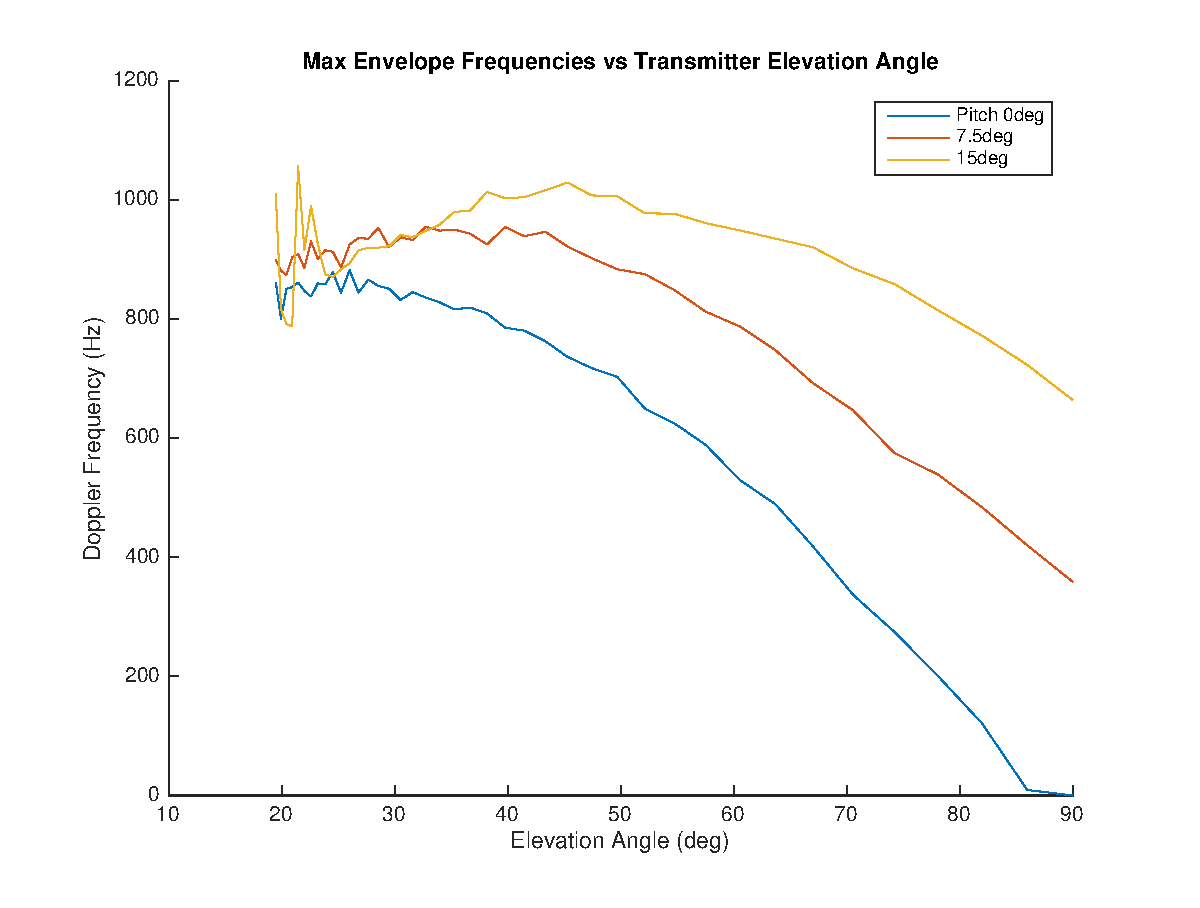
\includegraphics[width=10cm]{images/simulation/elevation_angle_with_pitch_max_doppler.eps}
		\caption{Max Envelope Frequencies vs Transmitter Elevation Angle}
		\label{fig:pitch_tx_elevation_angle}
	\end{center}
\end{figure}
%azimuth = 135deg

In figure \ref{fig:pitch_tx_elevation_angle} the max doppler vs elevation angles are initially shifted up in frequency from a pitch of 0 and has changed in slope. This is because the rays hitting the blades from below are reflecting into the receiver at an angle that is closer to the direction of blade travel. The interesting thing about this plot is that the pitch envelopes actually become closer to the 0\textdegree \space envelope as the elevation angle becomes smaller. Figure \ref{fig:pitch_tx_elevation_angle_difference} shows the difference plotted over elevation angle.

\begin{figure}
	\begin{center}
		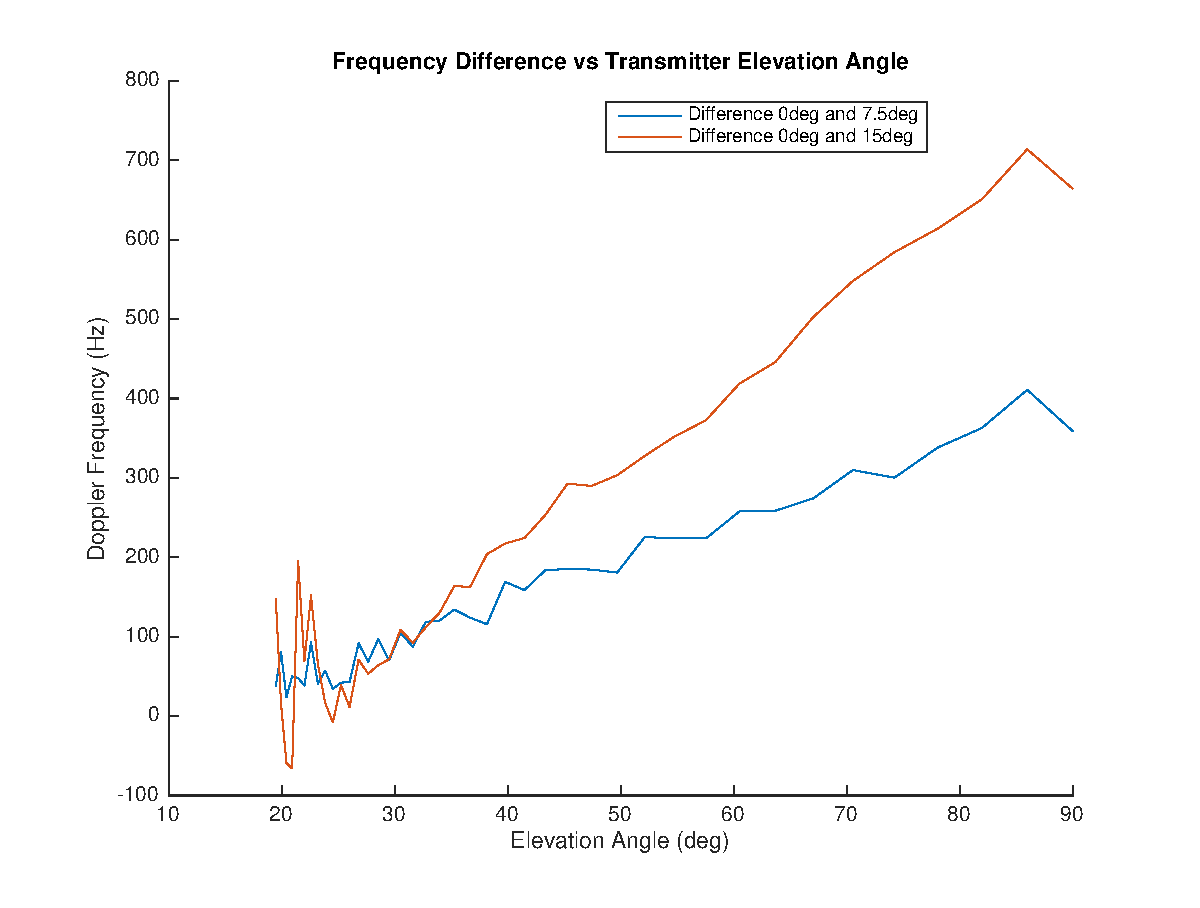
\includegraphics[width=10cm]{images/simulation/elevation_angle_with_pitch_max_doppler_Difference.eps}
		\caption{Frequency Difference vs Transmitter Elevation Angle}
		\label{fig:pitch_tx_elevation_angle_difference}
	\end{center}
\end{figure}

From figure \ref{fig:pitch_tx_elevation_angle_difference} we can see that the difference in frequency changes linearly as the elevation angle decreases, the slope of which is based on the pitch angle. This slope would have to be characterized on the physical craft and can be accounted for due to its predictable nature.

%-----------------------------------------------------------------------------------------------------------------------------------------------------------------------
\section{Transmitter Azimuth Angle} \label{taa}
%display azimuth angle with respect to max doppler readings and describe patterns
The transmitter azimuth angle corresponds to the cardinal direction of the transmitter with respect to the front of the helicopter.

%figure of azimuth angle positions
\begin{figure}
	\begin{center}
		\includegraphics[width=9cm]{images/simulation/azimuth.eps}
		\caption{Transmitter Azimuth Angle Relationship}
		\label{fig:tx_azimuth_rel}
	\end{center}
\end{figure}

Where $\theta_{Az}$ is the azimuth angle. The azimuth angle of the transmitter in the simulation will effect the amount of doppler added to the signal. This is due to the direction of the rotor blade rotation as it approaches both the receiver and the transmitter and how the rays reflect off the blade as it moves. From the model we see the amount of doppler form a sinusoidal pattern as the azimuth angle goes from $0$ to $2\pi$. This is mirrored in the simulation shown in figure \ref{fig:tx_azimuth_angle_200}.

%figure of doppler vs azimuth angle
\begin{figure}
	\begin{center}
		\includegraphics[width=10cm]{images/simulation/Azimuth_angle_200_max_doppler.eps}
		\caption{Max and Min Envelope Frequencies vs Transmitter Azimuth Angle with Tx Elevation at 45\textdegree}
		\label{fig:tx_azimuth_angle_200}
	\end{center}
\end{figure}
%azimuth variable, elevation = 45deg

The graph in figure \ref{fig:tx_azimuth_angle_200} shows both the max and the minimum measured doppler as the azimuth angle completes a full rotation. The doppler frequency follows the azimuth angle in a sinusoidal fashion. The sinusoidal pattern is held as the elevation angle changes shown in figures \ref{fig:tx_azimuth_angle_50} and \ref{fig:tx_azimuth_angle_400}.

%figure of doppler and azimuth angle for different elevation angles.
\begin{figure}
	\begin{center}
		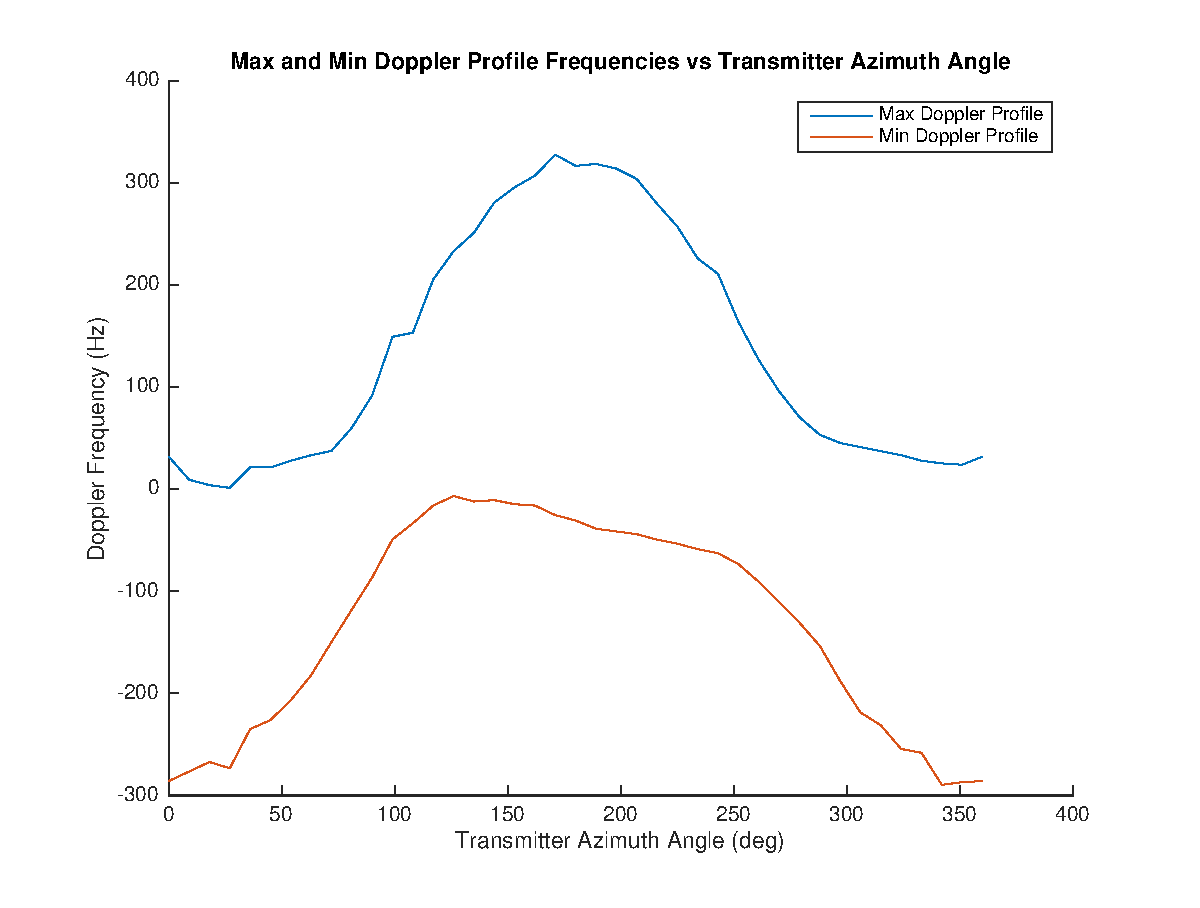
\includegraphics[width=10cm]{images/simulation/Azimuth_angle_50_max_doppler.eps}
		\caption{Max and Min Envelope Frequencies vs Transmitter Azimuth Angle with Tx Elevation at 76\textdegree}
		\label{fig:tx_azimuth_angle_50}
	\end{center}
\end{figure}
%azimuth variable, elevation = 76deg

\begin{figure}
	\begin{center}
		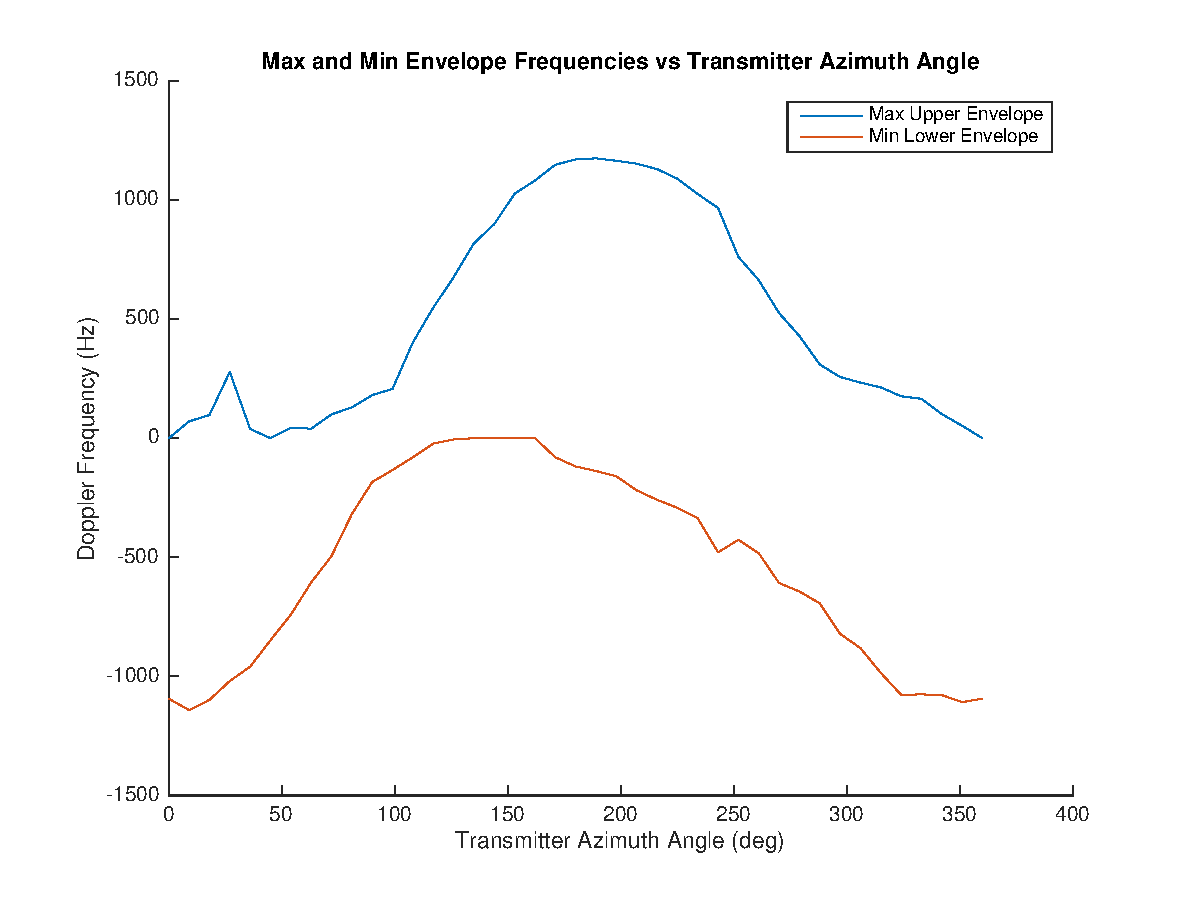
\includegraphics[width=10cm]{images/simulation/Azimuth_angle_400_max_doppler.eps}
		\caption{Max and Min Envelope Frequencies vs Transmitter Azimuth Angle with Tx Elevation at 26.5\textdegree}
		\label{fig:tx_azimuth_angle_400}
	\end{center}
\end{figure}
%azimuth variable, elevation = 26.5deg

%description
The sinusoidal pattern of min and max doppler frequencies are only present when the receiver is located away from the axis of rotation. This is shown in figure \ref{fig:tx_azimuth_rx0} which is devoid of any sinusoidal pattern and remains constant as the transmitter azimuth angle is changed. 

%figure of 0 rx position
\begin{figure}
	\begin{center}
		\includegraphics[width=10cm]{images/simulation/Azimuth_angle_rx0_max_doppler.eps}
		\caption{Max and Min Envelope Frequencies vs Transmitter Azimuth Angle with Rx at Axis of Rotation}
		\label{fig:tx_azimuth_rx0}
	\end{center}
\end{figure}

Therefore all future simulations will set the receiver near the tip of the rotor which would simulate the receiver being in the nose of the helicopter.

The effect of pitching the blade is that it modifies the results of the azimuth sweep when compared to figure \ref{fig:tx_azimuth_angle_200}. The resulting min and max envelope frequencies vs azimuth angle for pitch are shown in \ref{fig:pitch_azimuth_rev}. This occurs because the pitch of the blade angles RF reflections more in the direction of travel but not at all points in the azimuth. When the transmitter is located between 90\textdegree and 270\textdegree pitch causes an increase in doppler but elsewhere decreases the amount of doppler shift. The decrease is caused by the blade surface top reflecting receding doppler away from the receiver at those angles.

%azimuth pitch effect
\begin{figure}
	\begin{center}
		\includegraphics[width=10cm]{images/simulation/pitch_azimuth_rev.eps}
		\caption{Max and Min Envelope Frequencies vs Transmitter Elevation Angle with 7.5deg Pitch}
		\label{fig:pitch_azimuth_rev}
	\end{center}
\end{figure}

The effect of azimuth angle on the maximum measured doppler will be characterized in section \ref{sec:transmitter_azimuth_angle_estimation}

%-----------------------------------------------------------------------------------------------------------------------------------------------------------------------
\section{Transmitter Elevation Angle} \label{sec:tea}
%display elevation angle with respect to max doppler readings and describe patterns
The transmitter elevation angle is the angle between the helicopter rotor and the position of the transmitter shown in figure \ref{fig:azimuth_rel}.

%figure of position of elevation angle with respect to rotor
\begin{figure}
	\begin{center}
		\includegraphics[width=10cm]{images/simulation/elevation.eps}
		\caption{Transmitter Elevation Angle}
		\label{fig:azimuth_rel}
	\end{center}
\end{figure}

Where $\theta_{El}$ is the elevation angle. 

The smaller elevation angles mean that the transmitter is farther away from the helicopter. The elevation angle in relation to the distance of the transmitter is shown by figure \ref{fig:tx_range_elevation_rel}.

%figure of range vs elevation angle.
 \begin{figure}
	\begin{center}
		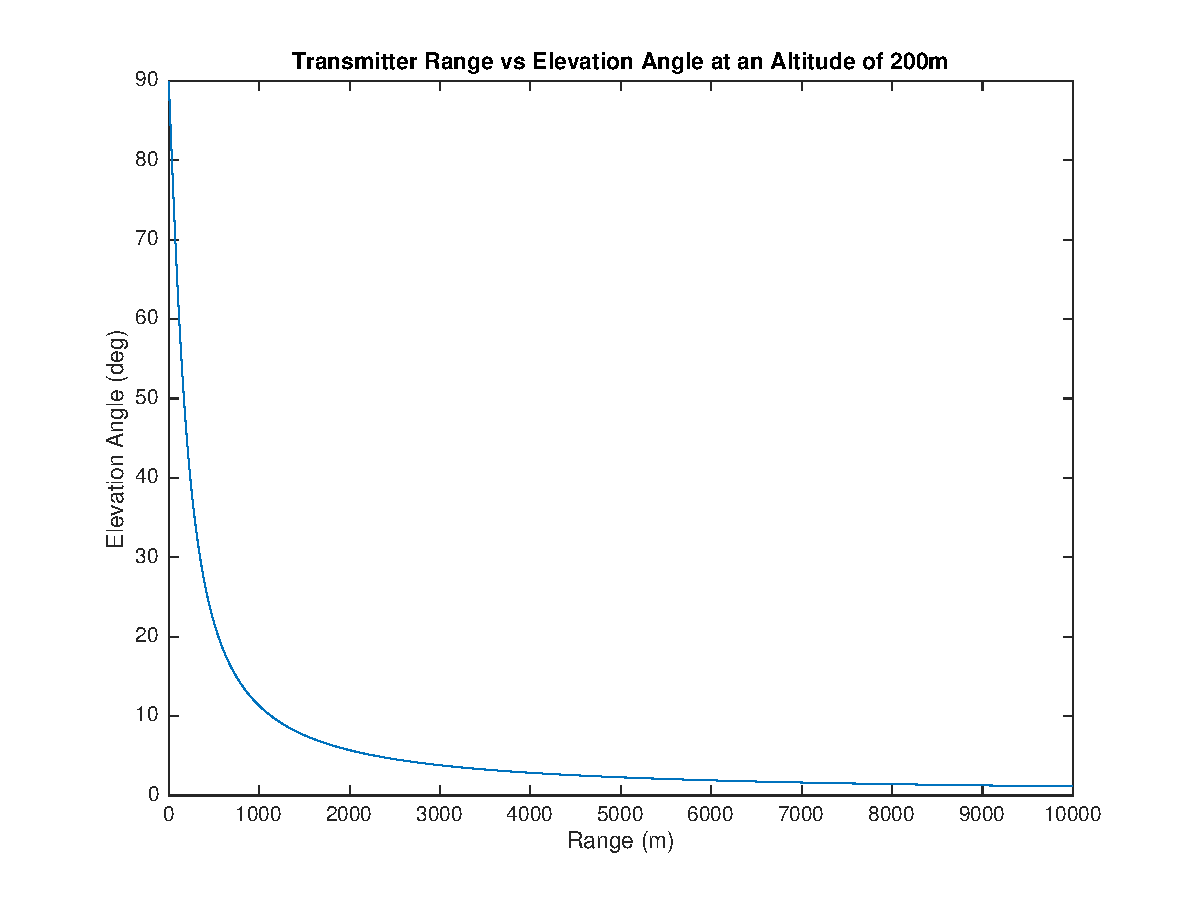
\includegraphics[width=10cm]{images/simulation/range_elevation_rel.eps}
		\caption{Transmitter Range vs Elevation Angle at an Altitude of 200m}
		\label{fig:tx_range_elevation_rel}
	\end{center}
\end{figure}

The elevation angle of the transmitter in the simulation will effect the amount of doppler added to the signal. This is due to the rays having a vector component in the direction of the travel of the rotor. When the transmitter is directly underneath the rotor and receiver there is no vector component in the direction of rotor travel so the reflected signal is not doppler shifted. From the model we see the amount of doppler increase as the elevation angle decreases. This is mirrored in the simulation shown in figure \ref{fig:tx_elevation_135deg}.

%figure of doppler vs (elevation angle)
 \begin{figure}
	\begin{center}
		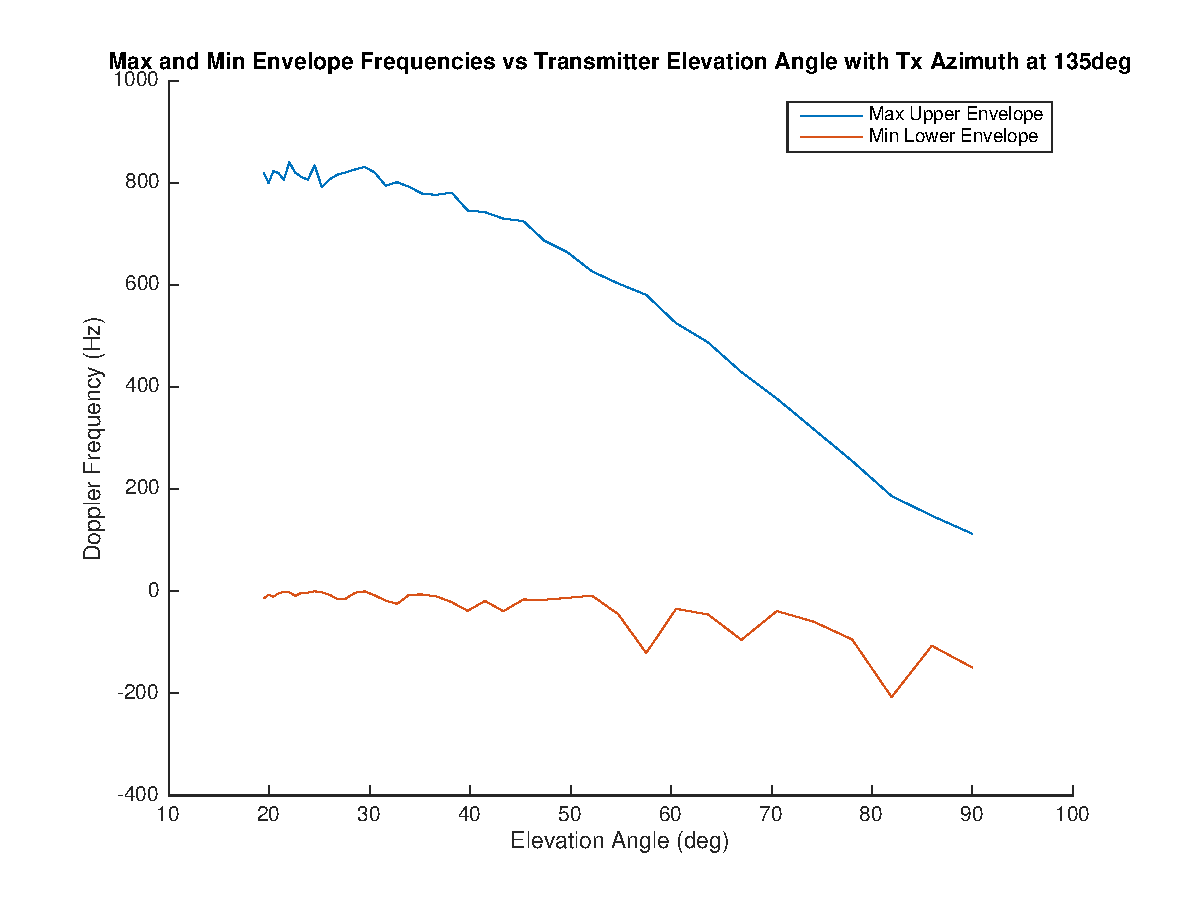
\includegraphics[width=10cm]{images/simulation/elevation_angle_max_doppler_135deg.eps}
		\caption{Max and Min Envelope Frequencies vs Transmitter Elevation Angle with Tx Azimuth of 135deg}
		\label{fig:tx_elevation_135deg}
	\end{center}
\end{figure}
%azimuth = 135deg, elevation = var

The graph in figure \ref{fig:tx_elevation_135deg} shows the maximum measured doppler as the elevation angle increases. 

Looking back at the geometric models for transmitter azimuth angles of 0\textdegree \space, 90\textdegree \space, 180\textdegree \space, and 270\textdegree \space and their simulated counterparts shown in figure \ref{fig:verify}.

\begin{figure}
\centering
	\subfloat[0\textdegree]{
	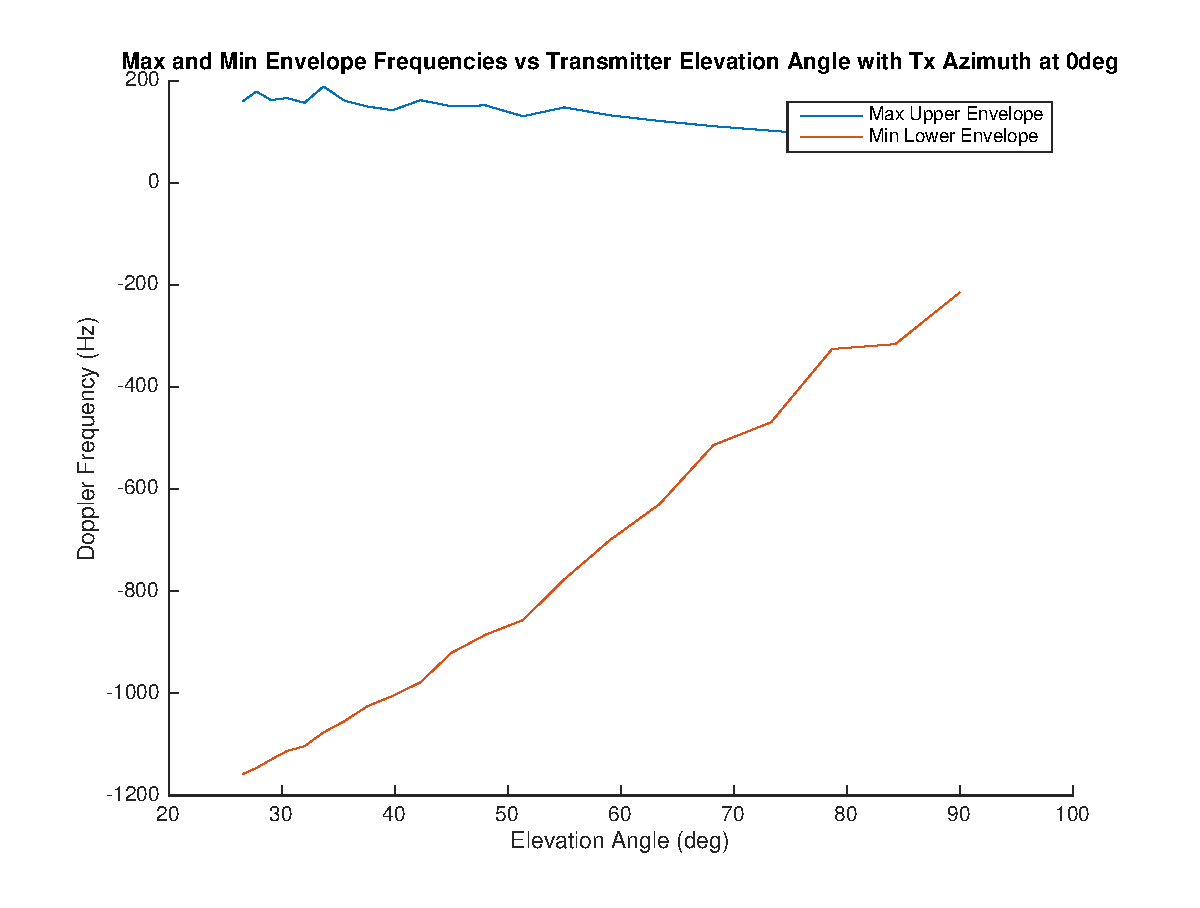
\includegraphics[width=7cm]{images/simulation/elevation_angle_max_doppler_0deg.eps}
	}
	\subfloat[90\textdegree]{
	\includegraphics[width=7cm]{images/simulation/elevation_angle_max_doppler_90deg.eps}
	}
	\newline
	\subfloat[180\textdegree]{
	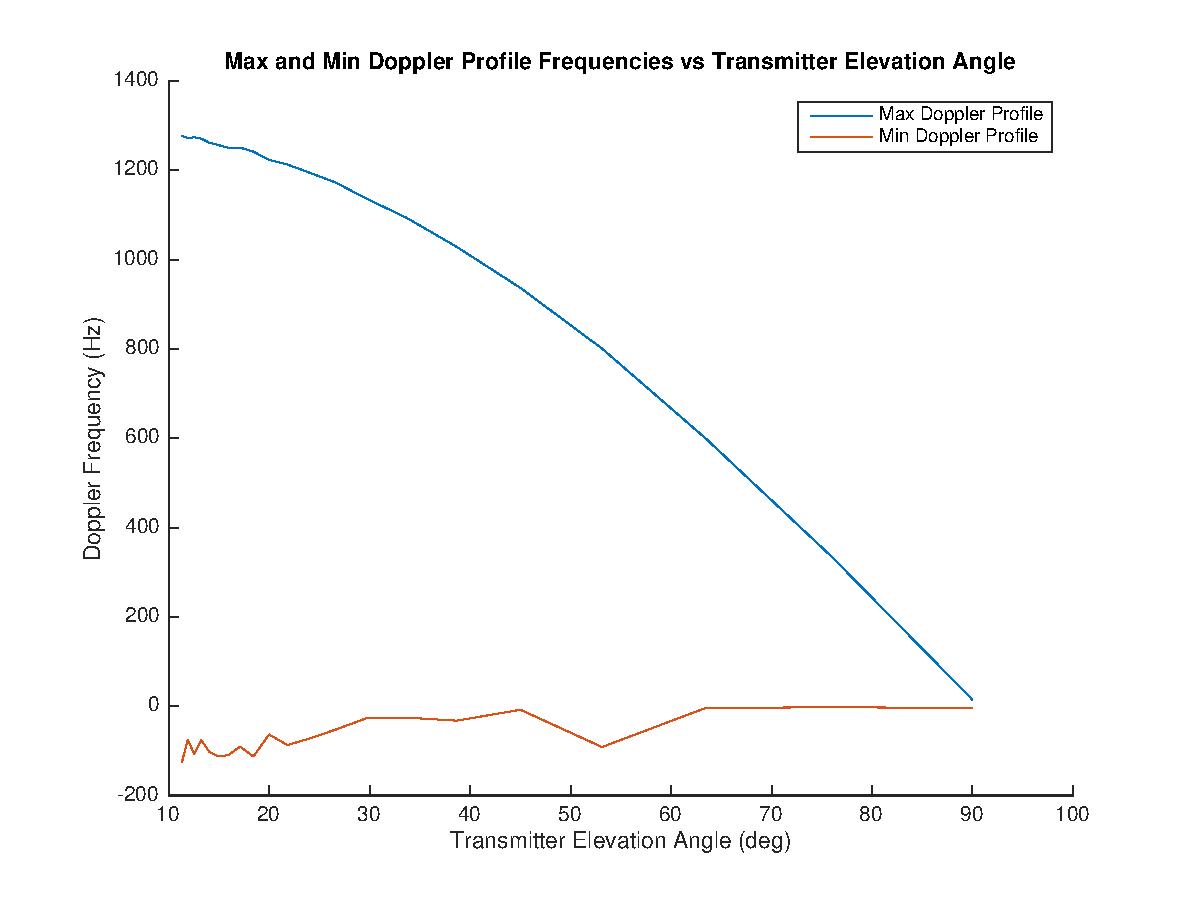
\includegraphics[width=7cm]{images/simulation/elevation_angle_max_doppler_180deg.eps}
	}
	\subfloat[270\textdegree]{
	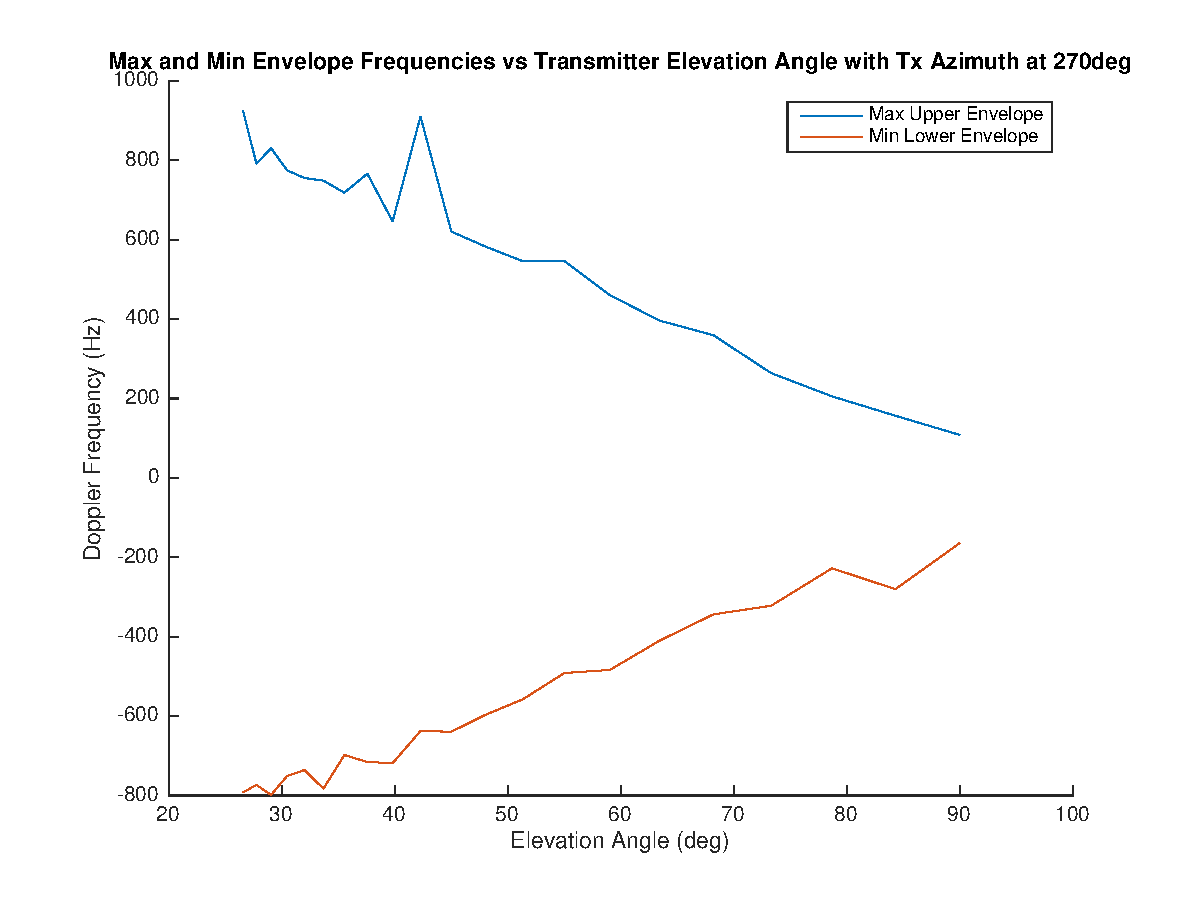
\includegraphics[width=7cm]{images/simulation/elevation_angle_max_doppler_270deg.eps}
	}
\caption{Doppler Profile vs. Transmitter Elevation angle for various Azimuth angles.}
\label{fig:verify}
\end{figure}

The effect of elevation angle on the maximum measured doppler will be characterized in section \ref{sec:transmitter_elevation_angle_estimation}.






\clearpage  %Start a new page
\lhead{\emph{Results}}
\chapter{Results}

\section{Introduction}
%introduce the results section and what processing will be done
The information gathered from the previous section is used to estimate the azimuth and elevation angles of the transmitter. First the azimuth angle will be estimated which will provide the information necessary for calculating the elevation angle. The results of the estimation techniques are then analyzed to determine their accuracy compared to the actual.

%-----------------------------------------------------------------------------------------------------------------------------------------------------------------------

\section{Transmitter Azimuth Angle Estimation}
%formulate the estimation equation and discuss ambiguity considerations
The azimuth angle estimation technique is based on the data collected by rotating the helicopter platform in a clockwise manner, during which at a set angle a doppler envelope is calculated and subsequent maximum and minimum values are collected. After a complete rotation the doppler maximum and minimum values produce a sinusoidal pattern as shown in figure \ref{fig:tx_azimuth_angle_200} without the assumption of knowing the starting azimuth angle. With this data we need to find an unambiguous angle that will set the coordinate space and provide an estimate of current azimuth angle. To do this the absolute value of the minimum envelope data is superimposed onto the maximum envelope data as shown in figure \ref{fig:azimuth_estimation_max_vs_absMin}.

\begin{figure}
	\begin{center}
		\includegraphics[width=10cm]{images/results/Azimuth_angle_estimation_max_vs_absMin.eps}
		\caption{Max and Absolute value of Min Envelope Frequencies vs Transmitter Azimuth Angle at an Elevation Angle of 45\textdegree}
		\label{fig:azimuth_estimation_max_vs_absMin}
	\end{center}
\end{figure}

From figure \ref{fig:azimuth_estimation_max_vs_absMin} there are two points at which the maximums and the absolute value of the minimums cross. By computing the difference \ref{eqn:difference}

%formula for difference
\begin{equation}
	 Envelope Difference = Max Upper Envelope - | Min Lower Envelope |
	 \label{eqn:difference}
\end{equation}

we produce an almost exact sinusoid centered around zero, shown in figure \ref{fig:azimuth_estimation_difference}.

 \begin{figure}[b]
	\begin{center}
		\includegraphics[width=10cm]{images/results/Azimuth_angle_estimation_difference.eps}
		\caption{Difference between Max and Min Envelope Calculations vs Transmitter Azimuth Angle at an Elevation Angle of 45\textdegree}
		\label{fig:azimuth_estimation_difference}
	\end{center}
\end{figure}

While figure \ref{fig:azimuth_estimation_difference} provides information about the angle of the transmitter it does not contain enough to locate an unambiguous azimuth angle in itself, therefore by computing the correct doppler to use from the $Max Upper Envelope$ and the $| Min Lower Envelope |$. This is done by evaluating the difference at each angle and if the difference is negative the $| Min Lower Envelope |$ is used and if positive the $Max Upper Envelope$.

%matlab for corrected doppler
\begin{lstlisting}
%corrected Doppler frequency for processing
for i = 1:length(upper)
    if(difference(i) < 0)
       correct_fd(i) = abs(lower(i));
    else
       correct_fd(i) = upper(i);
    end
end
\end{lstlisting}

\begin{figure}
	\begin{center}
		\includegraphics[width=10cm]{images/results/Correct_doppler.eps}
		\caption{Correct Doppler Frequencies vs Transmitter Azimuth Angle at an Elevation Angle of 45\textdegree}
		\label{fig:correct_fd}
	\end{center}
\end{figure}

The correct Doppler is shown in figure \ref{fig:correct_fd} which displays the amount of doppler that is currently acting on the signal for that specific azimuth angle. The data gathered contains a global minimum at 90\textdegree \space and a second local minimum at 270\textdegree. The 90\textdegree \space can be found easily by taking the minimum of the correct Doppler signal

%matlab minimum code
\begin{lstlisting}
%Minimum of corrected Doppler
[Min,I_min] = min(correct_fd);
\end{lstlisting}

%figure of minimum located vs azimuth
\begin{figure}
	\begin{center}
		\includegraphics[width=10cm]{images/results/Correct_doppler_with_Minumum.eps}
		\caption{Correct Doppler Frequencies with Minimum vs Transmitter Azimuth Angle at an Elevation Angle of 45\textdegree}
		\label{fig:min_correct_fd}
	\end{center}
\end{figure}

But in order to find the local minimum at 270\textdegree \space we need to use a different method. To do this we can use the peak detection function within Matlab to locate both the 90\textdegree and 270\textdegree point. By taking the inverse of the correct Doppler and tuning the peak detection function with the maximum and minimum values to determine accurate prominence.

%matlab peak detection code with tuning params
\begin{lstlisting}
%peak detection with prominence calculation
min_peak_prominence = (1/(Max - Min))*.5;
[pk,lc] = findpeaks(1./correct_fd, 'NPeaks', 2, 'MinPeakProminence', min_peak_prominence);
\end{lstlisting}

%figure with peak detection plotted vs azimuth
\begin{figure}
	\begin{center}
		\includegraphics[width=10cm]{images/results/Correct_doppler_inverse_peaks.eps}
		\caption{Peaks of inverted Correct Doppler vs Transmitter Azimuth Angle at an Elevation Angle of 45\textdegree}
		\label{fig:peaks}
	\end{center}
\end{figure}

From figure \ref{fig:peaks}  we see the two peaks denoted by the red x's, one at 90\textdegree \space and the other at  270\textdegree. Now we have a minimum value that should denote the 90\textdegree \space location and the two peak locations that denote the 90\textdegree \space 270\textdegree locations. Because it is possible that the minimum could find the wrong peak for the 90\textdegree \space location we can compare the peak locations on the average power data, that was used to find the successive average during data collection, to determine which location is actually 90\textdegree.

%figure with power plot with 90 and 270 denoted
\begin{figure}
	\begin{center}
		\includegraphics[width=10cm]{images/results/average_power_vs_Azimuth.eps}
		\caption{Average Power vs Transmitter Azimuth Angle at an Elevation Angle of 45\textdegree}
		\label{fig:ave_power}
	\end{center}
\end{figure}

Figure \ref{fig:ave_power}  shows the average power at each angle sample with the angles 90\textdegree \space and 270\textdegree denoted. From the plot we can see that the average power at 90\textdegree \space is much smaller than the the power at 270\textdegree, so this inequality will be used to resolve ambiguity in the azimuth angle. 

From there the Minimum method and the peak method can be compared to see if they agree on the 90\textdegree \space location. If this is not the case one will be chosen and the helicopter can fly in that direction and measure based on the physical movement of the helicopter or if the resulting envelope got larger or smaller because of the change in elevation angle.

%azimuth error table
\begin{table}
\begin{center}
    \begin{tabular}{ | l | l | l | l |}
    \hline
    Altitude & Elevation Angle & Azimuth Error in (deg) & Percent Error \\ \hline
     200 & 76\textdegree & 0 & 0  \\ \hline
     200 & 45\textdegree & 0 & 0  \\ \hline 
     200 & 26.5\textdegree & 0 & 0  \\ \hline
     500 & 78.7\textdegree & 0 & 0  \\ \hline
     500 & 51.34\textdegree & 0 & 0  \\ \hline 
     500 & 35.5\textdegree & 0 & 0  \\ \hline
    \end{tabular}
     \caption{Azimuth Error and Azimuth Percent Error of Different Elevation Angles During Azimuth Estimation}
    \label{tab:az_error_and_percent}
\end{center}
\end{table}

From table \ref{tab:az_error_and_percent} we can see that there is no error in the estimation of the 90\textdegree \space point over a variety of Altitude and elevation angles that were tested. But because of the algorithm could potentially pick the 270\textdegree we will analyze the difference in peak heights and the power difference to evaluate the estimation further.

\begin{table}
\begin{center}
    \begin{tabular}{ | l | l | p{3cm} | p{3cm} | p{3cm} |}
    \hline
    Altitude & Elevation Angle & Percent Peak Difference & Power Difference in dB & Peak Frequency Difference Hz\\ \hline
     200 & 76\textdegree & -16.8675\% & -14.0914  & 18.67 \\ \hline
     200 & 45\textdegree & -39.1124\% & -19.7476  &  176.267\\ \hline 
     200 & 26.5\textdegree & -69.7368\% & -13.3443 & 424.0 \\ \hline
     500 & 78.7\textdegree & -21.6667\% & -11.4508  & 17.33 \\ \hline
     500 & 51.34\textdegree & -38.1875\% & -22.4610  & 162.93 \\ \hline 
     500 & 35.5\textdegree & -53.4303\% & -18.6043  & 313.6 \\ \hline
    \end{tabular}
    \caption{Percent Peak, Power, and Frequency Difference of Different Elevation Angles During Azimuth Estimation}
    \label{tab:peaks_and_power}
\end{center}
\end{table}

From table \ref{tab:peaks_and_power} we can see that at the larger elevation angles the peak percent difference are significant to determine which is correctly the 90\textdegree value, but from the Peak frequency difference at the large elevation angles the difference is in the tens of Hz so in practical applications it is possible to confuse the estimation by just taking the minimum frequency so other values need to play a role such as the power.

%-----------------------------------------------------------------------------------------------------------------------------------------------------------------------

\section{Transmitter Elevation Angle Estimation}
%formulate the estimation equation and discuss ambiguity considerations
Using the information gathered from the azimuth estimation procedure we can compute the elevation angle of the transmitter. In the process of gathering azimuth information the maximum and minimum envelopes follow a sinusoidal pattern that contains a maximum Doppler information at approximately 180\textdegree \space and 0\textdegree \space azimuth angles. Using that maximum value along with the correct Doppler and the assumption that the maximum will occur near the tip of the rotor blade we can approximate the respected reflection radii off the blade as the azimuth angle changes. This is done through 
%reflection radius aproximation equation
\begin{equation}
	R_{Estimate} = BladeLength \left(\frac{f_{DopplerCorrect}(\theta_{Az})}{Max(f_{DopplerCorrect})}\right)
	\label{eqn:r_estimate}
\end{equation}

where $R_{Estimate}$ is the estimated reflection radius at a particular azimuth, $BladeLength$ is the length of a single blade or radius of the rotor, and $f_{DopplerCorrect}$ is the correct doppler frequency for each azimuth angle $\theta_{Az}$.

%figure of radius estimation 
\begin{figure}
	\begin{center}
		\includegraphics[width=10cm]{images/results/Estimated_reflection_radius_Azimuth_range.eps}
		\caption{Estimated Reflection Radius at an Elevation Angle of 45\textdegree}
		\label{fig:est_radius_azimuth_range}
	\end{center}
\end{figure}

Figure \ref{fig:est_radius_azimuth_range} shows the estimated reflection radius for each azimuth angle.

Now we find the maximum amount of Doppler that could be induced at that reflection radius location through
%max doppler at radius location
\begin{equation}
	f_{Doppler_{R Estimate Max}} = 2\frac{v_r f_c}{c}
	\label{eqn:max_doppler}
\end{equation}

where $f_{Doppler_{R Estimate Max}}$ is the maximum amount of doppler that could happen at that location if the signal was reflected parallel to the direction of motion. $f_c$ is the center frequency of the signal, $c$ is the speed of light and $v_r$ is the radial velocity based of the $RPM$ defined by

%radial velocity
\begin{equation}
	v_r = \frac{2\pi}{60} RPM R_{Estimate}
	\label{eqn:v_radial}
\end{equation}

Then to find the elevation angle we look back at equation (-) where we then solve for the elevation angle 
%Elevation angle
\begin{equation}
	\theta_{El} = acos\left(\frac{f_{DopplerCorrect(\theta_{Az})}}{f_{Doppler_{R Estimate Max}}}\right)
	\label{eqn:elevation_angle}
\end{equation}

where $\theta_{El}$ is the elevation angle of the transmitter. If the elevation angle is all the information needed equation \ref{eqn:elevation_angle} distills down to

%Elevation angle
\begin{equation}
	\theta_{El} = acos\left(\frac{Max(f_{DopplerCorrect})}{f_{DopplerMax}}\right)
	\label{eqn:elevation_angle_only}
\end{equation}

%figure of elevation angle 
\begin{figure}
	\begin{center}
		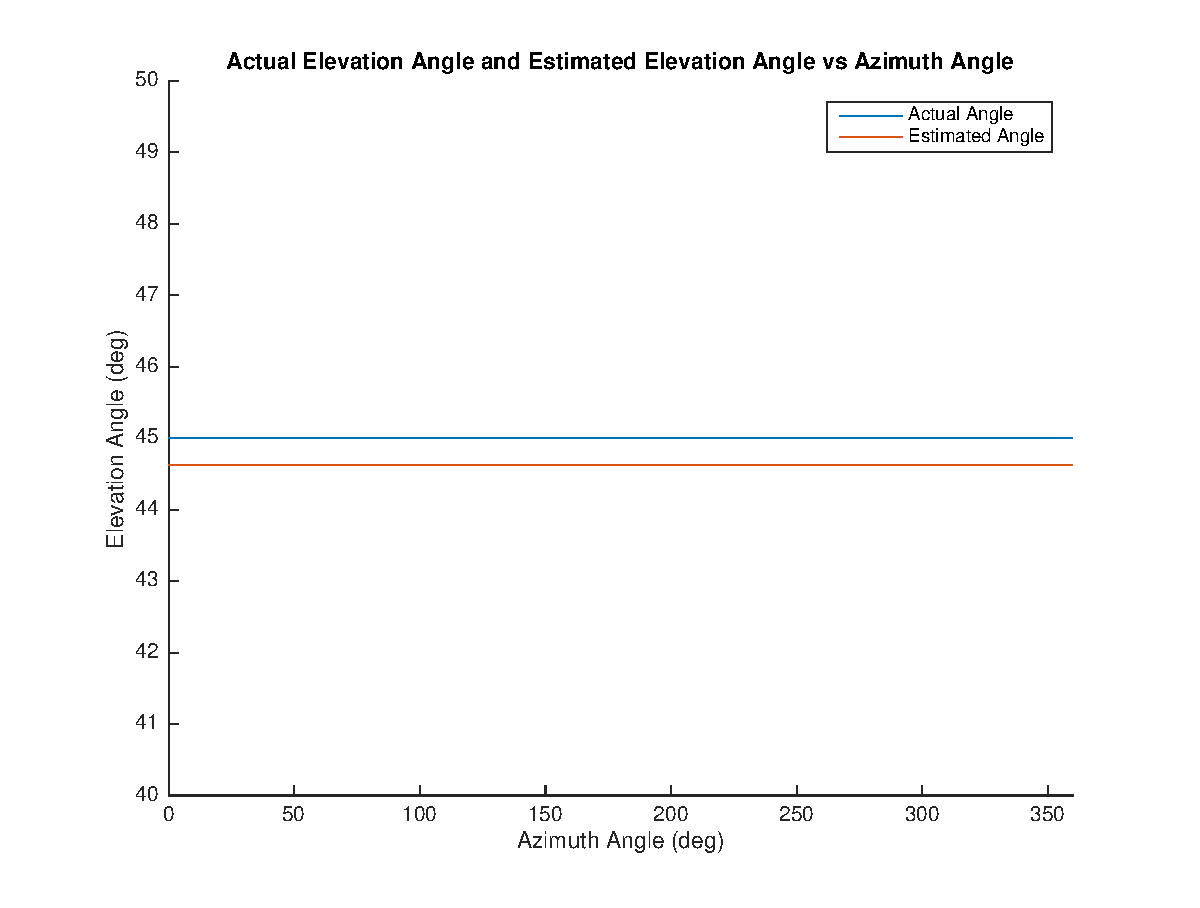
\includegraphics[width=10cm]{images/results/Elevation_angle_comparason_Azimuth_range.eps}
		\caption{Actual Elevation Angle and Estimated Elevation Angle vs Azimuth Angle}
		\label{fig:elevation_comparason_azimuth_range}
	\end{center}
\end{figure}

Figure \ref{fig:elevation_comparason_azimuth_range} shows the estimation of the elevation angle $\theta_{El}$ with respect to the azimuth angle, what it shows is that the elevation angle remains constant with respect to azimuth angle. which means that the estimation in the reflection radius is correctly compensating for the azimuth angle. The percent error off the actual elevation angle is shown in figure \ref{fig:percent_error_elevation_azimuth_range} which is very small and consistent over the azimuth range.

%figure of percent error
\begin{figure}
	\begin{center}
		\includegraphics[width=10cm]{images/results/Elevation_angle_percent_error_Azimuth_range.eps}
		\caption{Elevation Angle Percent Error vsTransmitter Azimuth Angle}
		\label{fig:percent_error_elevation_azimuth_range}
	\end{center}
\end{figure}

% Elevation error table
\begin{table}
\begin{center}
    \begin{tabular}{ | l | l | l | l |}
    \hline
    Altitude & Elevation Angle & Average Elevation Error in (deg) & Average Percent Error \\ \hline
     200 & 76\textdegree & -0.4632\textdegree & -0.6097\%  \\ \hline
     200 & 45\textdegree & -0.3809\textdegree & -0.8464\%  \\ \hline 
     200 & 26.5\textdegree & -0.4072\textdegree & -1.5329\%  \\ \hline
     500 & 78.7\textdegree & 0.0914\textdegree & 0.1162\% \\ \hline
     500 & 51.34\textdegree & -0.6236\textdegree & -1.2146\%  \\ \hline 
     500 & 35.5\textdegree & -0.6803\textdegree & -1.9143\%  \\ \hline
    \end{tabular}
    \caption{Average Elevation Error and Average Elevation Percent Error of Different Elevation Angles During Azimuth Estimation}
    \label{tab:elevation_error_percent}
\end{center}
\end{table}

From table \ref{tab:elevation_error_percent} elevation estimation error is extremely small for the given actual elevation angles. But there is a trend that is evident in the data that as the elevation angle decreases the amount of error is increasing.

%-----------------------------------------------------
% range limitations of this aproximation
%-----------------------------------------------------

This error is caused by a limitation on the estimation is that the doppler shift is limited by the maximum amount doppler that the blade rotation can produce shown in equation (-) by replacing $v_r$ with $v_rMax$ which is calculated by

%radial velocity
\begin{equation}
	v_{rMax} = \frac{2\pi}{60} RPM BladeLength
	\label{eqn:v_radial_max}
\end{equation}

then using that to find the maximum available doppler through

%maximum available doppler
\begin{equation}
	f_{DopplerMax} = 2\frac{v_{rMax} f_c}{c}
	\label{eqn:fd_max}
\end{equation}

This limitation is shown by varying the elevation angle at the azimuth angle that provides the maximum Doppler shift, which is 180\textdegree \space. The maximum and minimum envelope data is shown in figure \ref{fig:envelope_180deg}

%figure of 180 deg elevation sweep of envelope
\begin{figure}
	\begin{center}
		\includegraphics[width=10cm]{images/results/Elevation_angle_envelopes_180deg_Azimuth.eps}
		\caption{Max and Min Envelope Frequencies vs Elevation Angle with Transmitter Azimuth Angle of 180\textdegree}
		\label{fig:envelope_180deg}
	\end{center}
\end{figure}

%figure of comparing actual to estimated
\begin{figure}
	\begin{center}
		\includegraphics[width=10cm]{images/results/Elevation_angle_comparason_180deg_Azimuth.eps}
		\caption{Elevation Estimate and Actual Angle with Transmitter Azimuth Angle of 180\textdegree}
		\label{fig:angle_comparason_180deg}
	\end{center}
\end{figure}

Using the estimation method described above, figure \ref{fig:angle_comparason_180deg} shows the elevation angle estimated versus the actual angle. The estimation method is accurate till about 18\textdegree \space or 20\textdegree \space where it becomes noisy. This is due to the inability of the envelope estimation to resolve the correct maximum doppler for that range. By going back to figure (anglerangerelation) we can see that as the transmitter moves farther and farther away the elevation angle is still decreasing but at a much smaller and smaller rate. So the difference between elevation angles closer to zero are more difficult to resolve. 

%figure percent error of increasing error and variability
\begin{figure}
	\begin{center}
		\includegraphics[width=10cm]{images/results/Elevation_angle_percent_error_180deg_Azimuth.eps}
		\caption{Elevation Angle Percent Error with Transmitter Azimuth Angle of 180\textdegree}
		\label{fig:percent_error_elevation_180deg}
	\end{center}
\end{figure}

Figure \ref{fig:percent_error_elevation_180deg} shows the percent error with respect to the elevation angle and it starts to become unusable around 18\textdegree \space or 20\textdegree \space where the percent error starts to shoot past acceptable ranges.











\clearpage  %Start a new page
\lhead{\emph{Conclusion and Future Work}}
\chapter{Conclusion and Future Work} \label{ch:conclusion}

\section{Summary}

Over the course of this thesis a three dimensional ray tracer application was built in C++ to produce a RBM signal according to a variety of physical parameters. The physical parameters associated with a helicopter blade and the positioning of transmitter and receiver hardware were swept independently to build knowledge on how they affect the resulting signal. That data was then processed using time frequency analysis to produce a Doppler envelope. An envelope of each parameter step was used to determine an overall trend. Then with those trends an algorithm was derived to find the azimuth and elevation angle of the transmitter with relationship to the helicopter platform. The algorithm accurately finds the azimuth angle and elevation using the data collected in the simulation environment with little error in the azimuth estimation and less than 2\% error in elevation angle when blade pitch in 0\textdegree under a deterministic signal. With the addition of Gaussian noise the algorithm stays relatively constant up to a certain point, then both the azimuth and elevation estimations start to degrade with decreasing elevation angle and increasing noise level. For the simulation scenarios conducted, once the level of noise exceeded 10dB the algorithm started to degrade, but this level will most likely change if other simulation parameters are chosen.

\section{Future Work}
%Real world experiment needs to be conducted starting with small scale and moving towards a large scale implementation on a helicopter platform.
The first thing that needs to be done in continuing this research is to perform a real world experiment to officially evaluate the ray tracing application. To do this appropriate hardware needs to be defined in the form of a software defined radio for both the receiver and transmitter along with a software workflow such as GNU Radio. Next a small scale environment would need to be set up, with some form of rotating metal blade or thin plate rotating at a sufficient rate to produce a Doppler spread similar to those defined in the simulation. After that data is collected and analyzed a full scale experiment would need to be conducted including a real helicopter platform and an environment with large expanses of flat ground.

%Evaluate the estimation techniques on the real world collected data to see if they are still applicable.
Once the real world experiments have been conducted, and are shown to be similar to the signal produced by the simulation, the estimation techniques defined in this thesis can be evaluated on the real signal to determine if they are sufficient in practice.

%Improve propagation model to better represent the real world conditions, material, more physical effects on RF, near field problems etc.
After the physical validation the ray tracing application can be modified to include more physical phenomenon. The other improvement would be to introduce more objects into the scene model which would require modification to the tracing algorithm to include ray casting distributions in their particular direction.

%Improve computation speed by employing multithreading or computation on GPU Architecture for reduced simulation time, not necessary but would be more convenient.
Another improvement on the simulation would be to increase the speed of computation. This could be done by implementing multi-threading or, since raytracing is heavily parallelizable, a Graphics Processing Unit (GPU) based architecture. The multi-threading option would require minor code modifications but realizing the simulation on a GPU would require a full rewrite of the software to take advantage of the GPU's abilities. 

%Introduce a pitch parameter to the estimation equation based on empirical data, so that if the blades are pitched the doppler can be adjusted accordingly.
The current estimation does not take into account the physical pitch value when correcting for pitch and might not cover all the cases that pitch can effect. Therefore further investigation is needed into how the pitch affects the received signal for improved azimuth and elevation estimation.

%Because there is more information in the received envelopes besides the maximum and minimum the specific shape could be used to better estimate azimuth and elevation without the need to complete a full revolution as described in the proposed method.
The estimation methods described in this thesis rely only on the maximum and minimum values of the Doppler envelopes calculated but their shape could also be of particular interest as well. When varying the parameters of azimuth and elevation the shape of the envelope changes in a distinctive manner, by using a training algorithm the position of the transmitter might be able to be tracked in time by evaluating the change in shape. Under the defined estimation methods a full revolution of the helicopter platform is needed to resolve position ambiguity.
 



\clearpage  %Start a new page

%% ----------------------------------------------------------------
% Now begin the Appendices, including them as separate files

\addtocontents{toc}{\vspace{2em}} % Add a gap in the Contents, for aesthetics

\appendix % Cue to tell LaTeX that the following 'chapters' are Appendices

\lhead{\emph{Ray Tracing Software}}
\chapter{Ray Tracing Software}
something for code reuse and the git hub stuff

\lhead{\emph{Class Documentation}}
\chapter{Class Documentation}
\hypertarget{class_blade__surface}{}\section{Blade\+\_\+surface Class Reference}
\label{class_blade__surface}\index{Blade\+\_\+surface@{Blade\+\_\+surface}}


Collaboration diagram for Blade\+\_\+surface\+:
\nopagebreak
\begin{figure}[H]
\begin{center}
\leavevmode
\includegraphics[width=211pt]{doxygen/latex/class_blade__surface__coll__graph}
\end{center}
\end{figure}
\subsection*{Public Member Functions}
\begin{DoxyCompactItemize}
\item 
\hypertarget{class_blade__surface_a0c1a5fa3ea94afa451043ce70d3d7c1e}{}\label{class_blade__surface_a0c1a5fa3ea94afa451043ce70d3d7c1e} 
{\bfseries Blade\+\_\+surface} (const int id, const double length, const int Rib\+\_\+count, \hyperlink{class_rib}{Rib} \&origin\+\_\+\+Rib)
\item 
\hypertarget{class_blade__surface_a160959f632ad73eff846aeea81aa84ae}{}\label{class_blade__surface_a160959f632ad73eff846aeea81aa84ae} 
void {\bfseries create\+\_\+surface} ()
\item 
\hypertarget{class_blade__surface_a34d1f584602a5513960b0647a337232b}{}\label{class_blade__surface_a34d1f584602a5513960b0647a337232b} 
void {\bfseries update\+\_\+surface} ()
\item 
\hypertarget{class_blade__surface_a1eddf9a97aa9c2f4f399d03623e9fb6c}{}\label{class_blade__surface_a1eddf9a97aa9c2f4f399d03623e9fb6c} 
void {\bfseries update\+\_\+bounding\+\_\+box} ()
\item 
\hypertarget{class_blade__surface_a8d08aa093ce9eb861d5061303cc35a3b}{}\label{class_blade__surface_a8d08aa093ce9eb861d5061303cc35a3b} 
void {\bfseries rotate\+\_\+surface\+\_\+Z} (double angle)
\item 
\hypertarget{class_blade__surface_a384b9627c130a436d944264fb001d25b}{}\label{class_blade__surface_a384b9627c130a436d944264fb001d25b} 
void {\bfseries pitch\+\_\+surface\+\_\+X} (const double angle)
\item 
\hypertarget{class_blade__surface_a6823c31d12449828939ddc88ddb23705}{}\label{class_blade__surface_a6823c31d12449828939ddc88ddb23705} 
void {\bfseries height\+\_\+surface\+\_\+Z} (const double height)
\item 
\hypertarget{class_blade__surface_a1d4bc10f18e1ee2002a3fa1b5b0c0cb7}{}\label{class_blade__surface_a1d4bc10f18e1ee2002a3fa1b5b0c0cb7} 
bool {\bfseries hit} (const \hyperlink{class_ray3_d}{Ray3D} \&ray, double \&hit\+Distance, \hyperlink{class_vector3_d}{Vector3D} \&hit\+Normal, \hyperlink{class_point3_d}{Point3D} \&hit\+Point)
\item 
\hypertarget{class_blade__surface_a9d55669ccf429e408ff492cfecf52b6b}{}\label{class_blade__surface_a9d55669ccf429e408ff492cfecf52b6b} 
std\+::vector$<$ \hyperlink{class_rib}{Rib} $>$ {\bfseries get\+Ribs} ()
\item 
\hypertarget{class_blade__surface_a91f5bbe72574182ee6ad9e4014bfebbf}{}\label{class_blade__surface_a91f5bbe72574182ee6ad9e4014bfebbf} 
std\+::vector$<$ \hyperlink{class_triangle}{Triangle} $>$ {\bfseries get\+Surface} ()
\item 
\hypertarget{class_blade__surface_ae2f4aa670e4d320d63c77feffb953ae0}{}\label{class_blade__surface_ae2f4aa670e4d320d63c77feffb953ae0} 
std\+::vector$<$ \hyperlink{class_point3_d}{Point3D} $>$ {\bfseries get\+Points} ()
\item 
\hypertarget{class_blade__surface_a72fcd5b6eeb88c4e18da0ad267b27a93}{}\label{class_blade__surface_a72fcd5b6eeb88c4e18da0ad267b27a93} 
\hyperlink{class_bounding__box}{Bounding\+\_\+box} {\bfseries get\+Box} ()
\end{DoxyCompactItemize}
\subsection*{Public Attributes}
\begin{DoxyCompactItemize}
\item 
\hypertarget{class_blade__surface_afd3c87a82f107470cea4d3c8c1f5ee78}{}\label{class_blade__surface_afd3c87a82f107470cea4d3c8c1f5ee78} 
int {\bfseries id}
\item 
\hypertarget{class_blade__surface_a23f1ef284f842b523cb4b44235c0cdd7}{}\label{class_blade__surface_a23f1ef284f842b523cb4b44235c0cdd7} 
double {\bfseries length}
\item 
\hypertarget{class_blade__surface_ab1e364b4402fa787dea7d3b601e33778}{}\label{class_blade__surface_ab1e364b4402fa787dea7d3b601e33778} 
double {\bfseries delta\+\_\+l}
\item 
\hypertarget{class_blade__surface_a9ff7e20545a1fbb7ad84b00adb35f070}{}\label{class_blade__surface_a9ff7e20545a1fbb7ad84b00adb35f070} 
int {\bfseries Rib\+\_\+count}
\item 
\hypertarget{class_blade__surface_af1982ac4bb6460c4bae24868bd93e8d5}{}\label{class_blade__surface_af1982ac4bb6460c4bae24868bd93e8d5} 
\hyperlink{class_rib}{Rib} {\bfseries origin\+\_\+\+Rib}
\end{DoxyCompactItemize}


The documentation for this class was generated from the following files\+:\begin{DoxyCompactItemize}
\item 
Raytracer3\+D/\+Raytracer3\+D/Blade\+\_\+surface.\+hpp\item 
Raytracer3\+D/\+Raytracer3\+D/Blade\+\_\+surface.\+cpp\end{DoxyCompactItemize}

\hypertarget{class_bounding__box}{}\section{Bounding\+\_\+box Class Reference}
\label{class_bounding__box}\index{Bounding\+\_\+box@{Bounding\+\_\+box}}


Collaboration diagram for Bounding\+\_\+box\+:
\nopagebreak
\begin{figure}[H]
\begin{center}
\leavevmode
\includegraphics[width=180pt]{doxygen/latex/class_bounding__box__coll__graph}
\end{center}
\end{figure}
\subsection*{Public Member Functions}
\begin{DoxyCompactItemize}
\item 
\hypertarget{class_bounding__box_adf45c090850ee7b48b59f8e586450ef3}{}\label{class_bounding__box_adf45c090850ee7b48b59f8e586450ef3} 
{\bfseries Bounding\+\_\+box} (std\+::vector$<$ \hyperlink{class_point3_d}{Point3D} $>$ \&points)
\item 
\hypertarget{class_bounding__box_a29a6d043ac2de9fb152f39c1139e42df}{}\label{class_bounding__box_a29a6d043ac2de9fb152f39c1139e42df} 
bool {\bfseries hit} (const \hyperlink{class_ray3_d}{Ray3D} \&ray, \hyperlink{class_point3_d}{Point3D} \&hit\+\_\+point) const
\item 
\hypertarget{class_bounding__box_af2a1aa9cee9c82c2dd2df602cca9f42f}{}\label{class_bounding__box_af2a1aa9cee9c82c2dd2df602cca9f42f} 
bool {\bfseries hit} (const \hyperlink{class_ray3_d}{Ray3D} \&ray) const
\end{DoxyCompactItemize}
\subsection*{Public Attributes}
\begin{DoxyCompactItemize}
\item 
\hypertarget{class_bounding__box_add720cf740129c859bddbbed01727c48}{}\label{class_bounding__box_add720cf740129c859bddbbed01727c48} 
\hyperlink{class_point3_d}{Point3D} {\bfseries min\+\_\+point}
\item 
\hypertarget{class_bounding__box_a1ee058e226dbf771065c67d62cac8c66}{}\label{class_bounding__box_a1ee058e226dbf771065c67d62cac8c66} 
\hyperlink{class_point3_d}{Point3D} {\bfseries max\+\_\+point}
\end{DoxyCompactItemize}


The documentation for this class was generated from the following files\+:\begin{DoxyCompactItemize}
\item 
Raytracer3\+D/\+Raytracer3\+D/Bounding\+\_\+box.\+hpp\item 
Raytracer3\+D/\+Raytracer3\+D/Bounding\+\_\+box.\+cpp\end{DoxyCompactItemize}

\hypertarget{class_point3_d}{}\section{Point3D Class Reference}
\label{class_point3_d}\index{Point3D@{Point3D}}


Collaboration diagram for Point3D\+:
\nopagebreak
\begin{figure}[H]
\begin{center}
\leavevmode
\includegraphics[width=161pt]{doxygen/latex/class_point3_d__coll__graph}
\end{center}
\end{figure}
\subsection*{Public Member Functions}
\begin{DoxyCompactItemize}
\item 
\hypertarget{class_point3_d_a72799f11be08ba98bb37cfcf2fa0bb1f}{}\label{class_point3_d_a72799f11be08ba98bb37cfcf2fa0bb1f} 
{\bfseries Point3D} (const double x, const double y, const double z)
\item 
\hypertarget{class_point3_d_af963fbdffd449c8fc2d0631992a996e1}{}\label{class_point3_d_af963fbdffd449c8fc2d0631992a996e1} 
{\bfseries Point3D} (const double y, const double z)
\item 
\hypertarget{class_point3_d_a7ac9d9c06fe0497d868537d2f6ad9454}{}\label{class_point3_d_a7ac9d9c06fe0497d868537d2f6ad9454} 
\hyperlink{class_point3_d}{Point3D} {\bfseries operator-\/} () const
\item 
\hypertarget{class_point3_d_a6cb0fe83bc148a42fb2cf6f9aa907242}{}\label{class_point3_d_a6cb0fe83bc148a42fb2cf6f9aa907242} 
\hyperlink{class_vector3_d}{Vector3D} {\bfseries operator-\/} (const \hyperlink{class_point3_d}{Point3D} \&p) const
\item 
\hypertarget{class_point3_d_a2ab1c2f322e1845e94414fab67139667}{}\label{class_point3_d_a2ab1c2f322e1845e94414fab67139667} 
\hyperlink{class_point3_d}{Point3D} {\bfseries operator+} (const \hyperlink{class_vector3_d}{Vector3D} \&v) const
\item 
\hypertarget{class_point3_d_a376bb34529614f69a1d79b9633b6ab03}{}\label{class_point3_d_a376bb34529614f69a1d79b9633b6ab03} 
\hyperlink{class_point3_d}{Point3D} {\bfseries operator-\/} (const \hyperlink{class_vector3_d}{Vector3D} \&v) const
\item 
\hypertarget{class_point3_d_a30f07cec680e5e619289ba0c36c00d34}{}\label{class_point3_d_a30f07cec680e5e619289ba0c36c00d34} 
\hyperlink{class_point3_d}{Point3D} {\bfseries operator$\ast$} (const double a) const
\item 
\hypertarget{class_point3_d_a80016919138ae619c4ae603e0c963460}{}\label{class_point3_d_a80016919138ae619c4ae603e0c963460} 
bool {\bfseries operator==} (const \hyperlink{class_point3_d}{Point3D} \&p) const
\item 
\hypertarget{class_point3_d_a3db617345c47ecf25cee2d8bb08712dc}{}\label{class_point3_d_a3db617345c47ecf25cee2d8bb08712dc} 
double {\bfseries distance} (const \hyperlink{class_point3_d}{Point3D} \&p) const
\item 
\hypertarget{class_point3_d_aa2c65a74cd2605f2f46cd7fa88ed537c}{}\label{class_point3_d_aa2c65a74cd2605f2f46cd7fa88ed537c} 
double {\bfseries x} () const
\item 
\hypertarget{class_point3_d_aeeea1fe4bd6b56727b50c569b71f8207}{}\label{class_point3_d_aeeea1fe4bd6b56727b50c569b71f8207} 
double {\bfseries y} () const
\item 
\hypertarget{class_point3_d_ad663c810a730a64d1e000e366fc366ea}{}\label{class_point3_d_ad663c810a730a64d1e000e366fc366ea} 
double {\bfseries z} () const
\item 
\hypertarget{class_point3_d_a02de7d72811aef8bfc6660dd99267682}{}\label{class_point3_d_a02de7d72811aef8bfc6660dd99267682} 
void {\bfseries rotate\+\_\+Z} (const double angle)
\item 
\hypertarget{class_point3_d_aa282f1dc3a75839d0581583f89eeb1ea}{}\label{class_point3_d_aa282f1dc3a75839d0581583f89eeb1ea} 
void {\bfseries rotate\+\_\+X} (const double angle)
\item 
\hypertarget{class_point3_d_af415dc7a082ad664812b02df15902217}{}\label{class_point3_d_af415dc7a082ad664812b02df15902217} 
void {\bfseries translate\+\_\+Z} (const double height)
\end{DoxyCompactItemize}
\subsection*{Friends}
\begin{DoxyCompactItemize}
\item 
\hypertarget{class_point3_d_a84c3d7aa704e44e7f6cfbfe0cb6528f7}{}\label{class_point3_d_a84c3d7aa704e44e7f6cfbfe0cb6528f7} 
void {\bfseries swap} (\hyperlink{class_point3_d}{Point3D} \&a, \hyperlink{class_point3_d}{Point3D} \&b)
\end{DoxyCompactItemize}


The documentation for this class was generated from the following files\+:\begin{DoxyCompactItemize}
\item 
Raytracer3\+D/\+Raytracer3\+D/Point3d.\+hpp\item 
Raytracer3\+D/\+Raytracer3\+D/Point3d.\+cpp\end{DoxyCompactItemize}

\hypertarget{class_ray3_d}{}\section{Ray3D Class Reference}
\label{class_ray3_d}\index{Ray3D@{Ray3D}}


Collaboration diagram for Ray3D\+:
\nopagebreak
\begin{figure}[H]
\begin{center}
\leavevmode
\includegraphics[width=254pt]{doxygen/latex/class_ray3_d__coll__graph}
\end{center}
\end{figure}
\subsection*{Public Member Functions}
\begin{DoxyCompactItemize}
\item 
\hypertarget{class_ray3_d_a0cd2092288763fc6c0fd8dccebf11527}{}\label{class_ray3_d_a0cd2092288763fc6c0fd8dccebf11527} 
{\bfseries Ray3D} (const \hyperlink{class_point3_d}{Point3D} \&origin, const \hyperlink{class_vector3_d}{Vector3D} \&direction, const double power=1.\+0, const double frequency=0.\+0, const double distance=0)
\end{DoxyCompactItemize}
\subsection*{Public Attributes}
\begin{DoxyCompactItemize}
\item 
\hypertarget{class_ray3_d_aa303389d0d8e8569f4bdef420e850717}{}\label{class_ray3_d_aa303389d0d8e8569f4bdef420e850717} 
\hyperlink{class_point3_d}{Point3D} {\bfseries origin}
\item 
\hypertarget{class_ray3_d_a1b9fbe26d23a38f12be002d0e5990fd2}{}\label{class_ray3_d_a1b9fbe26d23a38f12be002d0e5990fd2} 
\hyperlink{class_vector3_d}{Vector3D} {\bfseries direction}
\item 
\hypertarget{class_ray3_d_adbe652ae6043219a7a6d22c3e6a454db}{}\label{class_ray3_d_adbe652ae6043219a7a6d22c3e6a454db} 
double {\bfseries power}
\item 
\hypertarget{class_ray3_d_a5be97a26ac4f733fee0b9a10ca78197a}{}\label{class_ray3_d_a5be97a26ac4f733fee0b9a10ca78197a} 
double {\bfseries frequency}
\item 
\hypertarget{class_ray3_d_a1287339cd3f7358590b2fb65dbb88505}{}\label{class_ray3_d_a1287339cd3f7358590b2fb65dbb88505} 
double {\bfseries distance}
\end{DoxyCompactItemize}


The documentation for this class was generated from the following files\+:\begin{DoxyCompactItemize}
\item 
Raytracer3\+D/\+Raytracer3\+D/Ray3d.\+hpp\item 
Raytracer3\+D/\+Raytracer3\+D/Ray3d.\+cpp\end{DoxyCompactItemize}

\hypertarget{class_receiver}{}\section{Receiver Class Reference}
\label{class_receiver}\index{Receiver@{Receiver}}


Collaboration diagram for Receiver\+:
\nopagebreak
\begin{figure}[H]
\begin{center}
\leavevmode
\includegraphics[width=195pt]{doxygen/latex/class_receiver__coll__graph}
\end{center}
\end{figure}
\subsection*{Public Member Functions}
\begin{DoxyCompactItemize}
\item 
\hypertarget{class_receiver_a94a089e687b5320f02b3000304ffd08c}{}\label{class_receiver_a94a089e687b5320f02b3000304ffd08c} 
{\bfseries Receiver} (const int id, const double Bandwidth, const double center\+\_\+freq, const \hyperlink{class_point3_d}{Point3D} \&center, const double boundary\+\_\+radius, const std\+::string \&savefile\+\_\+name, const std\+::string \&dopplerfile\+\_\+name)
\item 
\hypertarget{class_receiver_a6d0f579d480c7303d8138981e546ff01}{}\label{class_receiver_a6d0f579d480c7303d8138981e546ff01} 
\hyperlink{class_sphere}{Sphere} {\bfseries get\+\_\+\+Boundary} ()
\item 
\hypertarget{class_receiver_a6e97969b694ba385a495bf64f9adc16a}{}\label{class_receiver_a6e97969b694ba385a495bf64f9adc16a} 
double {\bfseries get\+\_\+sampling\+\_\+rate} ()
\item 
\hypertarget{class_receiver_a146b5c800df5f2e17eb89faa16a3929a}{}\label{class_receiver_a146b5c800df5f2e17eb89faa16a3929a} 
std\+::vector$<$ \hyperlink{class_ray3_d}{Ray3D} $>$ {\bfseries get\+\_\+frame\+\_\+data} ()
\item 
\hypertarget{class_receiver_aaa3ac7cecd33cba5a382fb0db441082e}{}\label{class_receiver_aaa3ac7cecd33cba5a382fb0db441082e} 
void {\bfseries save\+\_\+ray\+\_\+to\+Frame} (\hyperlink{class_ray3_d}{Ray3D} \&ray)
\item 
\hypertarget{class_receiver_a72ce8129ebd0720a810959eb0a47dfc8}{}\label{class_receiver_a72ce8129ebd0720a810959eb0a47dfc8} 
void {\bfseries save\+\_\+to\+\_\+file} ()
\end{DoxyCompactItemize}
\subsection*{Public Attributes}
\begin{DoxyCompactItemize}
\item 
\hypertarget{class_receiver_aaadfb4436bd66669d03811c846985843}{}\label{class_receiver_aaadfb4436bd66669d03811c846985843} 
int {\bfseries id}
\item 
\hypertarget{class_receiver_a19225a5d1c7c5f4cdaa36b99a1184d26}{}\label{class_receiver_a19225a5d1c7c5f4cdaa36b99a1184d26} 
double {\bfseries Bandwidth}
\item 
\hypertarget{class_receiver_a33f4396a9edddf6fe298108ffa12da58}{}\label{class_receiver_a33f4396a9edddf6fe298108ffa12da58} 
double {\bfseries center\+\_\+freq}
\item 
\hypertarget{class_receiver_a7cf7efbe8c86d8f585e744cbba86c267}{}\label{class_receiver_a7cf7efbe8c86d8f585e744cbba86c267} 
double {\bfseries Resolution}
\item 
\hypertarget{class_receiver_ad9a009e1e386791e5c3bd7211d83a3f9}{}\label{class_receiver_ad9a009e1e386791e5c3bd7211d83a3f9} 
double {\bfseries boundary\+\_\+radius}
\item 
\hypertarget{class_receiver_a4432a9eafa52a2483918d2d3119cb597}{}\label{class_receiver_a4432a9eafa52a2483918d2d3119cb597} 
\hyperlink{class_point3_d}{Point3D} {\bfseries center}
\end{DoxyCompactItemize}


The documentation for this class was generated from the following files\+:\begin{DoxyCompactItemize}
\item 
Raytracer3\+D/\+Raytracer3\+D/Receiver.\+hpp\item 
Raytracer3\+D/\+Raytracer3\+D/Receiver.\+cpp\end{DoxyCompactItemize}

\hypertarget{class_rib}{}\section{Rib Class Reference}
\label{class_rib}\index{Rib@{Rib}}


Collaboration diagram for Rib\+:
\nopagebreak
\begin{figure}[H]
\begin{center}
\leavevmode
\includegraphics[width=168pt]{doxygen/latex/class_rib__coll__graph}
\end{center}
\end{figure}
\subsection*{Public Member Functions}
\begin{DoxyCompactItemize}
\item 
\hypertarget{class_rib_a417cde052770f55f3344d785aef969ef}{}\label{class_rib_a417cde052770f55f3344d785aef969ef} 
{\bfseries Rib} (int id, \hyperlink{class_rib}{Rib} \&x, const double delta\+\_\+l)
\item 
\hypertarget{class_rib_aaaed7a2c960a33e5ac0c510ea7d8881c}{}\label{class_rib_aaaed7a2c960a33e5ac0c510ea7d8881c} 
{\bfseries Rib} (int id, const std\+::string \&filename)
\item 
\hypertarget{class_rib_ae4ea708286531b624f587f22b9416a36}{}\label{class_rib_ae4ea708286531b624f587f22b9416a36} 
std\+::vector$<$ \hyperlink{class_point3_d}{Point3D} $>$ {\bfseries get\+Rib\+Points} ()
\item 
\hypertarget{class_rib_ab6715214f4a43ed51b46a8f42d6f198b}{}\label{class_rib_ab6715214f4a43ed51b46a8f42d6f198b} 
void {\bfseries pitch} (double angle)
\item 
\hypertarget{class_rib_aafef170600416b0e6a86ccb4e8bd4e32}{}\label{class_rib_aafef170600416b0e6a86ccb4e8bd4e32} 
void {\bfseries rotate} (double angle)
\item 
\hypertarget{class_rib_a08859793a4800c7d160d0b494ad39af7}{}\label{class_rib_a08859793a4800c7d160d0b494ad39af7} 
void {\bfseries height} (const double height)
\end{DoxyCompactItemize}
\subsection*{Public Attributes}
\begin{DoxyCompactItemize}
\item 
\hypertarget{class_rib_ac88341591298af4d11837a09b47917d5}{}\label{class_rib_ac88341591298af4d11837a09b47917d5} 
int {\bfseries id}
\end{DoxyCompactItemize}


The documentation for this class was generated from the following files\+:\begin{DoxyCompactItemize}
\item 
Raytracer3\+D/\+Raytracer3\+D/Rib.\+hpp\item 
Raytracer3\+D/\+Raytracer3\+D/Rib.\+cpp\end{DoxyCompactItemize}

\hypertarget{class_rotor}{}\section{Rotor Class Reference}
\label{class_rotor}\index{Rotor@{Rotor}}


Collaboration diagram for Rotor\+:
\nopagebreak
\begin{figure}[H]
\begin{center}
\leavevmode
\includegraphics[width=196pt]{doxygen/latex/class_rotor__coll__graph}
\end{center}
\end{figure}
\subsection*{Public Member Functions}
\begin{DoxyCompactItemize}
\item 
\hypertarget{class_rotor_af922b65832291cafdb53c52a545ac136}{}\label{class_rotor_af922b65832291cafdb53c52a545ac136} 
double {\bfseries get\+\_\+\+R\+PM} ()
\item 
\hypertarget{class_rotor_a25eef55d0719b86a255d3aa09f7a2688}{}\label{class_rotor_a25eef55d0719b86a255d3aa09f7a2688} 
int {\bfseries get\+\_\+num\+\_\+blades} ()
\item 
\hypertarget{class_rotor_ad0c276d01564fbdda8ca63c7eff18df6}{}\label{class_rotor_ad0c276d01564fbdda8ca63c7eff18df6} 
double {\bfseries get\+\_\+height} ()
\item 
\hypertarget{class_rotor_a53d18f1d59a1c2b71cdb8c9cab0acd4c}{}\label{class_rotor_a53d18f1d59a1c2b71cdb8c9cab0acd4c} 
double {\bfseries get\+\_\+constant\+\_\+pitch} ()
\item 
\hypertarget{class_rotor_af384431ad8eba046b8541ac5d1a3f9f9}{}\label{class_rotor_af384431ad8eba046b8541ac5d1a3f9f9} 
double {\bfseries get\+\_\+\+Rib\+\_\+count} ()
\item 
\hypertarget{class_rotor_a43485a289837aab864e28dc00109fdf6}{}\label{class_rotor_a43485a289837aab864e28dc00109fdf6} 
double {\bfseries get\+\_\+blade\+\_\+length} ()
\item 
\hypertarget{class_rotor_a31c1b1a9674d87d0b612db4989a4ae16}{}\label{class_rotor_a31c1b1a9674d87d0b612db4989a4ae16} 
std\+::vector$<$ \hyperlink{class_blade__surface}{Blade\+\_\+surface} $>$ {\bfseries get\+\_\+\+Blades} ()
\item 
\hypertarget{class_rotor_ac73f8ab43793bc45b978c6ef14239a4c}{}\label{class_rotor_ac73f8ab43793bc45b978c6ef14239a4c} 
void {\bfseries rotate} (const double angle)
\item 
\hypertarget{class_rotor_ab1ecb2c8efc6e125db1fe9121c6c47b9}{}\label{class_rotor_ab1ecb2c8efc6e125db1fe9121c6c47b9} 
bool {\bfseries hit} (const \hyperlink{class_ray3_d}{Ray3D} \&ray, double \&hit\+Distance, \hyperlink{class_vector3_d}{Vector3D} \&hit\+Normal, \hyperlink{class_point3_d}{Point3D} \&hit\+Point)
\item 
\hypertarget{class_rotor_ad525c69ea4ba137f953675839befcaa6}{}\label{class_rotor_ad525c69ea4ba137f953675839befcaa6} 
{\bfseries Rotor} (const int id, const int num\+\_\+blades, const double R\+PM, const double height, const double constant\+\_\+pitch, const double blade\+\_\+length, const int Rib\+\_\+count)
\end{DoxyCompactItemize}
\subsection*{Public Attributes}
\begin{DoxyCompactItemize}
\item 
\hypertarget{class_rotor_abcb7f6ed3121a0734eef3763d4d20172}{}\label{class_rotor_abcb7f6ed3121a0734eef3763d4d20172} 
int {\bfseries id}
\end{DoxyCompactItemize}


The documentation for this class was generated from the following files\+:\begin{DoxyCompactItemize}
\item 
Raytracer3\+D/\+Raytracer3\+D/Rotor.\+hpp\item 
Raytracer3\+D/\+Raytracer3\+D/Rotor.\+cpp\end{DoxyCompactItemize}

\hypertarget{class_scene}{}\section{Scene Class Reference}
\label{class_scene}\index{Scene@{Scene}}


Collaboration diagram for Scene\+:
\nopagebreak
\begin{figure}[H]
\begin{center}
\leavevmode
\includegraphics[width=193pt]{doxygen/latex/class_scene__coll__graph}
\end{center}
\end{figure}
\subsection*{Public Member Functions}
\begin{DoxyCompactItemize}
\item 
\hypertarget{class_scene_a39f55da2de994a41500a2c0a3bbc207d}{}\label{class_scene_a39f55da2de994a41500a2c0a3bbc207d} 
{\bfseries Scene} (double rx\+\_\+x, double rx\+\_\+y, double rx\+\_\+z, double Bandwidth, double rx\+\_\+fc, double tx\+\_\+x, double tx\+\_\+y, double tx\+\_\+fc, double tx\+\_\+power, int num\+\_\+blades, double R\+PM, double altitude, double pitch, double blade\+\_\+length, int num\+\_\+ribs, const std\+::string \&filename)
\item 
\hypertarget{class_scene_a59d78e42eebf29106e413275abacf983}{}\label{class_scene_a59d78e42eebf29106e413275abacf983} 
\hyperlink{class_rotor}{Rotor} {\bfseries get\+\_\+rotor} ()
\item 
\hypertarget{class_scene_aeca85b3d6824c3509c94991136fe6a1b}{}\label{class_scene_aeca85b3d6824c3509c94991136fe6a1b} 
\hyperlink{class_transmitter}{Transmitter} {\bfseries get\+\_\+transmitter} ()
\item 
\hypertarget{class_scene_aea609d389de6e5c483d3e7f19a3aff0a}{}\label{class_scene_aea609d389de6e5c483d3e7f19a3aff0a} 
\hyperlink{class_receiver}{Receiver} {\bfseries get\+\_\+receiver} ()
\item 
\hypertarget{class_scene_a2d3012d31a139a597d50f5b84fbec51d}{}\label{class_scene_a2d3012d31a139a597d50f5b84fbec51d} 
void {\bfseries trace\+\_\+scene} (int num\+\_\+rays)
\item 
\hypertarget{class_scene_a26979e16c27d21bdd615c24c1c11902c}{}\label{class_scene_a26979e16c27d21bdd615c24c1c11902c} 
void {\bfseries trace\+\_\+vect} (\hyperlink{class_ray3_d}{Ray3D} \&test\+\_\+ray, double \&hit\+Distance, \hyperlink{class_vector3_d}{Vector3D} \&hit\+Normal, \hyperlink{class_point3_d}{Point3D} \&hit\+Point)
\item 
\hypertarget{class_scene_a9af282cee68bb4748bd15568bda0ecfb}{}\label{class_scene_a9af282cee68bb4748bd15568bda0ecfb} 
void {\bfseries update} (double angle)
\item 
\hypertarget{class_scene_a76fa370d0c210100d4cf8799474faa8d}{}\label{class_scene_a76fa370d0c210100d4cf8799474faa8d} 
double {\bfseries get\+Distance\+Power} (const double frequency, const double power, const double distance) const
\item 
double \hyperlink{class_scene_a969abe0e6022d73ff082d380c59d83f5}{get\+Doppler} (\hyperlink{class_ray3_d}{Ray3D} \&test\+\_\+ray, \hyperlink{class_vector3_d}{Vector3D} \&hit\+Normal, \hyperlink{class_point3_d}{Point3D} \&hit\+Point, double R\+PM) const
\end{DoxyCompactItemize}


\subsection{Member Function Documentation}
\hypertarget{class_scene_a969abe0e6022d73ff082d380c59d83f5}{}\label{class_scene_a969abe0e6022d73ff082d380c59d83f5} 
\index{Scene@{Scene}!get\+Doppler@{get\+Doppler}}
\index{get\+Doppler@{get\+Doppler}!Scene@{Scene}}
\subsubsection{\texorpdfstring{get\+Doppler()}{getDoppler()}}
{\footnotesize\ttfamily double Scene\+::get\+Doppler (\begin{DoxyParamCaption}\item[{\hyperlink{class_ray3_d}{Ray3D} \&}]{test\+\_\+ray,  }\item[{\hyperlink{class_vector3_d}{Vector3D} \&}]{hit\+Normal,  }\item[{\hyperlink{class_point3_d}{Point3D} \&}]{hit\+Point,  }\item[{double}]{R\+PM }\end{DoxyParamCaption}) const\hspace{0.3cm}{\ttfamily [inline]}}

!!!! doppler does not get affected by the normal, need to check this. not sure if this is correct. 

The documentation for this class was generated from the following files\+:\begin{DoxyCompactItemize}
\item 
Raytracer3\+D/\+Raytracer3\+D/Scene.\+hpp\item 
Raytracer3\+D/\+Raytracer3\+D/Scene.\+cpp\end{DoxyCompactItemize}

\hypertarget{class_sphere}{}\section{Sphere Class Reference}
\label{class_sphere}\index{Sphere@{Sphere}}


Collaboration diagram for Sphere\+:
\nopagebreak
\begin{figure}[H]
\begin{center}
\leavevmode
\includegraphics[width=161pt]{doxygen/latex/class_sphere__coll__graph}
\end{center}
\end{figure}
\subsection*{Public Member Functions}
\begin{DoxyCompactItemize}
\item 
\hypertarget{class_sphere_a7b5d0be5fd60ba94573e3941cf4eb094}{}\label{class_sphere_a7b5d0be5fd60ba94573e3941cf4eb094} 
{\bfseries Sphere} (const double radius, const \hyperlink{class_point3_d}{Point3D} \&center)
\item 
\hypertarget{class_sphere_a5da44ddc57c5a68a1092b0df86dc18cd}{}\label{class_sphere_a5da44ddc57c5a68a1092b0df86dc18cd} 
bool {\bfseries hit} (const \hyperlink{class_ray3_d}{Ray3D} \&ray, double \&hit\+Distance, \hyperlink{class_vector3_d}{Vector3D} \&hit\+Normal, \hyperlink{class_point3_d}{Point3D} \&hit\+Point) const
\end{DoxyCompactItemize}
\subsection*{Public Attributes}
\begin{DoxyCompactItemize}
\item 
\hypertarget{class_sphere_a45d6c6c870fac7c2a885ad2e226334ad}{}\label{class_sphere_a45d6c6c870fac7c2a885ad2e226334ad} 
double {\bfseries radius}
\item 
\hypertarget{class_sphere_a774cb90ed1b46592e63a112338f1cc58}{}\label{class_sphere_a774cb90ed1b46592e63a112338f1cc58} 
\hyperlink{class_point3_d}{Point3D} {\bfseries center}
\item 
\hypertarget{class_sphere_a50d3abf7b35058bae9bcbba998a82943}{}\label{class_sphere_a50d3abf7b35058bae9bcbba998a82943} 
int {\bfseries num\+\_\+points}
\end{DoxyCompactItemize}


The documentation for this class was generated from the following files\+:\begin{DoxyCompactItemize}
\item 
Raytracer3\+D/\+Raytracer3\+D/Sphere.\+hpp\item 
Raytracer3\+D/\+Raytracer3\+D/Sphere.\+cpp\end{DoxyCompactItemize}

\hypertarget{class_transmitter}{}\section{Transmitter Class Reference}
\label{class_transmitter}\index{Transmitter@{Transmitter}}


Collaboration diagram for Transmitter\+:
\nopagebreak
\begin{figure}[H]
\begin{center}
\leavevmode
\includegraphics[width=177pt]{doxygen/latex/class_transmitter__coll__graph}
\end{center}
\end{figure}
\subsection*{Public Member Functions}
\begin{DoxyCompactItemize}
\item 
\hypertarget{class_transmitter_a91c51bc1d7c42db81fb390753de5c0ea}{}\label{class_transmitter_a91c51bc1d7c42db81fb390753de5c0ea} 
{\bfseries Transmitter} (const int id, const double frequency, const double power, const \hyperlink{class_point3_d}{Point3D} \&center, const double l)
\item 
\hypertarget{class_transmitter_aa26f745526cba27666812ca7c05b9df7}{}\label{class_transmitter_aa26f745526cba27666812ca7c05b9df7} 
void {\bfseries set\+Power} (const double power)
\item 
\hypertarget{class_transmitter_a72eb7b0c29d6d5e3429f9920dcdf86c9}{}\label{class_transmitter_a72eb7b0c29d6d5e3429f9920dcdf86c9} 
double {\bfseries get\+Power} () const
\item 
\hypertarget{class_transmitter_a8a2727ad1e4b48ec9f64c0285bb5bd04}{}\label{class_transmitter_a8a2727ad1e4b48ec9f64c0285bb5bd04} 
\hyperlink{class_ray3_d}{Ray3D} {\bfseries make\+Ray} ()
\item 
\hypertarget{class_transmitter_a7c51cee738e95fb6f2af955986873b7c}{}\label{class_transmitter_a7c51cee738e95fb6f2af955986873b7c} 
\hyperlink{class_ray3_d}{Ray3D} {\bfseries make\+Ray\+\_\+disk} (const double height)
\item 
\hypertarget{class_transmitter_a5c6bdf0d0dd931f9f4282a7d585f2320}{}\label{class_transmitter_a5c6bdf0d0dd931f9f4282a7d585f2320} 
\hyperlink{class_ray3_d}{Ray3D} {\bfseries make\+Ray} (const \hyperlink{class_vector3_d}{Vector3D} \&ray\+Direction)
\end{DoxyCompactItemize}
\subsection*{Public Attributes}
\begin{DoxyCompactItemize}
\item 
\hypertarget{class_transmitter_a3e57cbedcf7ff80c3506c47d43119f5d}{}\label{class_transmitter_a3e57cbedcf7ff80c3506c47d43119f5d} 
int {\bfseries id}
\item 
\hypertarget{class_transmitter_ade036fee92a7f2aad8ecf206f89b8c34}{}\label{class_transmitter_ade036fee92a7f2aad8ecf206f89b8c34} 
double {\bfseries frequency}
\item 
\hypertarget{class_transmitter_a61c6aa4371c98b49d2d9277fd4447f34}{}\label{class_transmitter_a61c6aa4371c98b49d2d9277fd4447f34} 
\hyperlink{class_point3_d}{Point3D} {\bfseries center}
\item 
\hypertarget{class_transmitter_ac339f9fd3011afdbdc729b99b371e617}{}\label{class_transmitter_ac339f9fd3011afdbdc729b99b371e617} 
double {\bfseries power}
\end{DoxyCompactItemize}


The documentation for this class was generated from the following files\+:\begin{DoxyCompactItemize}
\item 
Raytracer3\+D/\+Raytracer3\+D/Transmitter.\+hpp\item 
Raytracer3\+D/\+Raytracer3\+D/Transmitter.\+cpp\end{DoxyCompactItemize}

\hypertarget{class_triangle}{}\section{Triangle Class Reference}
\label{class_triangle}\index{Triangle@{Triangle}}


Collaboration diagram for Triangle\+:
\nopagebreak
\begin{figure}[H]
\begin{center}
\leavevmode
\includegraphics[width=175pt]{doxygen/latex/class_triangle__coll__graph}
\end{center}
\end{figure}
\subsection*{Public Member Functions}
\begin{DoxyCompactItemize}
\item 
\hypertarget{class_triangle_a995e961620da6b595053ef5560999244}{}\label{class_triangle_a995e961620da6b595053ef5560999244} 
{\bfseries Triangle} (\hyperlink{class_point3_d}{Point3D} \&v0, \hyperlink{class_point3_d}{Point3D} \&v1, \hyperlink{class_point3_d}{Point3D} \&v2)
\item 
\hypertarget{class_triangle_ab09716ce6c0928ce11fe34091c19a1c4}{}\label{class_triangle_ab09716ce6c0928ce11fe34091c19a1c4} 
bool {\bfseries hit} (const \hyperlink{class_ray3_d}{Ray3D} \&ray, double \&hit\+Distance, \hyperlink{class_vector3_d}{Vector3D} \&hit\+Normal, \hyperlink{class_point3_d}{Point3D} \&hit\+Point) const
\item 
\hypertarget{class_triangle_a7b93ca1524b80830bf8ea07d660ace6a}{}\label{class_triangle_a7b93ca1524b80830bf8ea07d660ace6a} 
bool {\bfseries hit\+No\+Cull} (const \hyperlink{class_ray3_d}{Ray3D} \&ray, double \&hit\+Distance, \hyperlink{class_vector3_d}{Vector3D} \&hit\+Normal, \hyperlink{class_point3_d}{Point3D} \&hit\+Point) const
\item 
\hypertarget{class_triangle_aeeced29a75e5c27db3457804debbb936}{}\label{class_triangle_aeeced29a75e5c27db3457804debbb936} 
bool {\bfseries operator==} (\hyperlink{class_triangle}{Triangle} \&Tri)
\item 
\hypertarget{class_triangle_a7dbe3b94aae0c1966801d50190ab2c25}{}\label{class_triangle_a7dbe3b94aae0c1966801d50190ab2c25} 
\hyperlink{class_point3_d}{Point3D} {\bfseries get\+Vertex0} ()
\item 
\hypertarget{class_triangle_a88c0bdcbda9d290e7ea876714b634b83}{}\label{class_triangle_a88c0bdcbda9d290e7ea876714b634b83} 
\hyperlink{class_point3_d}{Point3D} {\bfseries get\+Vertex1} ()
\item 
\hypertarget{class_triangle_aa29a363ca196b8352c749174cfd0ebd9}{}\label{class_triangle_aa29a363ca196b8352c749174cfd0ebd9} 
\hyperlink{class_point3_d}{Point3D} {\bfseries get\+Vertex2} ()
\item 
\hypertarget{class_triangle_a30e9a577df2eb923fd8c869fc1958cd1}{}\label{class_triangle_a30e9a577df2eb923fd8c869fc1958cd1} 
\hyperlink{class_vector3_d}{Vector3D} {\bfseries get\+Normal} () const
\item 
\hypertarget{class_triangle_a557fd01902542dca2bccb3de38aa1534}{}\label{class_triangle_a557fd01902542dca2bccb3de38aa1534} 
void {\bfseries set\+Normal} (const \hyperlink{class_vector3_d}{Vector3D} \&normal)
\item 
\hypertarget{class_triangle_a1fe02e3810a30dca5e6ddf646f7f31a5}{}\label{class_triangle_a1fe02e3810a30dca5e6ddf646f7f31a5} 
void {\bfseries flip\+Normal} ()
\item 
\hypertarget{class_triangle_a8e187af2dd348e5c51a657ca066221ac}{}\label{class_triangle_a8e187af2dd348e5c51a657ca066221ac} 
\hyperlink{class_point3_d}{Point3D} {\bfseries centroid} () const
\item 
\hypertarget{class_triangle_a0e10ae200b1a7698a800ddfa06d8d00d}{}\label{class_triangle_a0e10ae200b1a7698a800ddfa06d8d00d} 
\hyperlink{class_point3_d}{Point3D} {\bfseries centroid\+XY} () const
\item 
\hypertarget{class_triangle_a0674ff79061f6413e6aa721e1ac5dd06}{}\label{class_triangle_a0674ff79061f6413e6aa721e1ac5dd06} 
void {\bfseries update\+Normal} ()
\end{DoxyCompactItemize}


The documentation for this class was generated from the following files\+:\begin{DoxyCompactItemize}
\item 
Raytracer3\+D/\+Raytracer3\+D/Triangle.\+hpp\item 
Raytracer3\+D/\+Raytracer3\+D/Triangle.\+cpp\end{DoxyCompactItemize}

\hypertarget{class_vector3_d}{}\section{Vector3D Class Reference}
\label{class_vector3_d}\index{Vector3D@{Vector3D}}


Collaboration diagram for Vector3D\+:
\nopagebreak
\begin{figure}[H]
\begin{center}
\leavevmode
\includegraphics[width=155pt]{doxygen/latex/class_vector3_d__coll__graph}
\end{center}
\end{figure}
\subsection*{Public Member Functions}
\begin{DoxyCompactItemize}
\item 
\hypertarget{class_vector3_d_a9c58f21ac5a280f62067d7f26466ba47}{}\label{class_vector3_d_a9c58f21ac5a280f62067d7f26466ba47} 
{\bfseries Vector3D} (const double x, const double y, const double z)
\item 
\hypertarget{class_vector3_d_a5fc1291699c792e6acd5ea453c47f3f4}{}\label{class_vector3_d_a5fc1291699c792e6acd5ea453c47f3f4} 
\hyperlink{class_vector3_d}{Vector3D} {\bfseries operator-\/} (void) const
\item 
\hypertarget{class_vector3_d_afa1d5717e088826b6dcc0cb35ec836f7}{}\label{class_vector3_d_afa1d5717e088826b6dcc0cb35ec836f7} 
\hyperlink{class_vector3_d}{Vector3D} {\bfseries operator$\ast$} (const double a) const
\item 
\hypertarget{class_vector3_d_a86a2dec32df2740e92e06b651d693c95}{}\label{class_vector3_d_a86a2dec32df2740e92e06b651d693c95} 
\hyperlink{class_vector3_d}{Vector3D} {\bfseries operator/} (const double a) const
\item 
\hypertarget{class_vector3_d_af75a42c25ca6e999f3e7a83d4de105c6}{}\label{class_vector3_d_af75a42c25ca6e999f3e7a83d4de105c6} 
\hyperlink{class_vector3_d}{Vector3D} {\bfseries operator+} (const \hyperlink{class_vector3_d}{Vector3D} \&v) const
\item 
\hypertarget{class_vector3_d_acd7927ced75a36b459200a791e51acad}{}\label{class_vector3_d_acd7927ced75a36b459200a791e51acad} 
\hyperlink{class_vector3_d}{Vector3D} {\bfseries operator-\/} (const \hyperlink{class_vector3_d}{Vector3D} \&v) const
\item 
\hypertarget{class_vector3_d_a307962a6472b58ac85af69ad74c4fd6f}{}\label{class_vector3_d_a307962a6472b58ac85af69ad74c4fd6f} 
double {\bfseries operator$\ast$} (const \hyperlink{class_vector3_d}{Vector3D} \&b) const
\item 
\hypertarget{class_vector3_d_ac6d8d994b5c80eaaed1f033fd7baa627}{}\label{class_vector3_d_ac6d8d994b5c80eaaed1f033fd7baa627} 
\hyperlink{class_vector3_d}{Vector3D} {\bfseries operator$^\wedge$} (const \hyperlink{class_vector3_d}{Vector3D} \&v) const
\item 
\hypertarget{class_vector3_d_ac86d9a556616f4c51fecbaf7d8658ce8}{}\label{class_vector3_d_ac86d9a556616f4c51fecbaf7d8658ce8} 
double {\bfseries x} () const
\item 
\hypertarget{class_vector3_d_a7146d35db2c1bf7606c8290282a423ec}{}\label{class_vector3_d_a7146d35db2c1bf7606c8290282a423ec} 
double {\bfseries y} () const
\item 
\hypertarget{class_vector3_d_af4ae427e82a23af845f804106daed509}{}\label{class_vector3_d_af4ae427e82a23af845f804106daed509} 
double {\bfseries z} () const
\item 
\hypertarget{class_vector3_d_af396bfa140d140d818a97100f7d6a532}{}\label{class_vector3_d_af396bfa140d140d818a97100f7d6a532} 
double {\bfseries dot\+Product} (const \hyperlink{class_vector3_d}{Vector3D} \&v) const
\item 
\hypertarget{class_vector3_d_a15b417a5abd07b8a7403bdb0ac5f95ec}{}\label{class_vector3_d_a15b417a5abd07b8a7403bdb0ac5f95ec} 
\hyperlink{class_vector3_d}{Vector3D} {\bfseries cross\+Product} (const \hyperlink{class_vector3_d}{Vector3D} \&v) const
\item 
\hypertarget{class_vector3_d_a4ddb90e85e10f0f32475725cb966a5ce}{}\label{class_vector3_d_a4ddb90e85e10f0f32475725cb966a5ce} 
double {\bfseries length} () const
\item 
\hypertarget{class_vector3_d_aac87aef508e65eb8ada23346b5e552c3}{}\label{class_vector3_d_aac87aef508e65eb8ada23346b5e552c3} 
\hyperlink{class_vector3_d}{Vector3D} {\bfseries normalized} () const
\item 
\hypertarget{class_vector3_d_a1698a0e33c975b78f0076b51331e6e94}{}\label{class_vector3_d_a1698a0e33c975b78f0076b51331e6e94} 
\hyperlink{class_vector3_d}{Vector3D} {\bfseries rotated\+AboutZ} (const double angle) const
\item 
\hypertarget{class_vector3_d_a5df051b736bdb50b63995442b0816938}{}\label{class_vector3_d_a5df051b736bdb50b63995442b0816938} 
bool {\bfseries is\+Normal} () const
\end{DoxyCompactItemize}


The documentation for this class was generated from the following files\+:\begin{DoxyCompactItemize}
\item 
Raytracer3\+D/\+Raytracer3\+D/Vector3d.\+hpp\item 
Raytracer3\+D/\+Raytracer3\+D/Vector3d.\+cpp\end{DoxyCompactItemize}


%\include{Simulation_Data}

%\chapter{Matlab Code}
add scripts that are most important

%\input{Appendices/AppendixA} % Appendix Title
%\input{Appendices/AppendixB} % Appendix Title
%\input{Appendices/AppendixC} % Appendix Title

\addtocontents{toc}{\vspace{2em}}  % Add a gap in the Contents, for aesthetics
\backmatter

%% ----------------------------------------------------------------
\label{Bibliography}
\lhead{\emph{Bibliography}}  % Change the left side page header to "Bibliography"
\bibliographystyle{IEEEtran}  % Use the "unsrtnat" BibTeX style for formatting the Bibliography
\bibliography{Bibliography}  % The references (bibliography) information are stored in the file named "Bibliography.bib"

\end{document}  % The End
%% ----------------------------------------------------------------